\chapter{Metodi}
\label{cha:metodi}

In questo capitolo verrà presentata l'architettura di rete utilizzata per lo scopo di ricerca e verranno discusse criticamente le tecniche di acquisizione, regressione e segmentazione dei dati utlizzate per condurre l'analisi.


\section{PhiNets}
\label{sec:phinet}

L'architettura delle PhiNets consiste in una famiglia di reti scalabile e ottimizzata per l’elaborazione delle immagini basata sul deep learning per piattaforme con risorse limitate. \cite{10.1145/3510832}

In particolare per i diversi compiti di classificazione di immagini, rilevamento e tracking in tempo reale di oggetti, le reti convoluzionali di questa famiglia si distinguono per la struttura dell'ultimo layer (classificatore o detection head), mantenendo però in comune il \textit{backbone}, ovvero l'insieme degli strati convolutivi atti all'estrazione delle feature. Per rendere tali modelli scalabili, è fondamentale ottimizzare il backbone della rete poichè esso è responsabile della maggior parte del consumo di risorse durante l'inferenza del modello. Le tecniche utilizzate a questo scopo riguardano principalmente lo sfruttamento di blocchi convoluzionali efficienti e l'utilizzo di un'architettura modificabile tramite degli opportuni fattori di scala.


\subsection{Blocchi convoluzionali}
La famiglia di reti delle PhiNets è particolarmente ottimizzata a livello computazionale grazie a delle specifiche operazioni di convoluzione utilizzate in ogni layer, vengono infatti impiegati gli \textit{inverted residual blocks}, ovvero dei blocchi convoluzionali efficienti introdotti in MobileNetV2. \cite{mobilenetv2}

Per poter apprezzare i benefici portati dall'introduzione di questo tipo di operazioni, bisogna prima comprendere il funzionamento dei \textit{residual blocks} tradizionali, implementati inzialmente nell'architettura delle ResNet \cite{ResNet}. Questi blocchi residuali prendono il nome dall'operazione di \textit{skip connection} che lega l'input e l'output dell'operazione convolutiva, la quale propaga dei residui della rappresentazione in entrata. Il funzionamento basilare prevede infatti la riduzione del numero di canali della feature map in ingresso al blocco tramite un'operazione convolutiva non dispendiosa, la successiva espansione del numero di canali (riportati al valore iniziale) tipicamente tramite una \textit{depthwise separable convolution} (sezione \ref{sec:mobilenets}) e l'applicazione della skip connection, che lascia dei residui della rappresentazione in input nella feature map in output. Questo tipo di blocco residuale riduce fortemente il numero di parametri ed il numero di operazioni effettuate dalla rete ma ne degrada anche le prestazioni. 

Proprio al fine di risolvere il problema di deterioramento delle performance di queste operazioni, sono stati introdotti gli \textit{inverted residual blocks} che mirano a bilanciare le prestazioni di rete rinunciando ad una parte del guadagno sul consumo di risorse. La procedura di funzionamento è molto simile a quella dei blocchi residuali tradizionali con la differenza che il numero di canali della rappresentazione in entrata viene inizialmente espanso, per poter estrarre informazioni più dettagliate, per poi essere compresso alla fine del blocco allo scopo di ottenere in uscita una rappresentazione con la stessa dimensionalità di quella in ingresso. A questa struttura di base del blocco residuale invertito, l'architettura delle PhiNets aggiunge un'operazione denominata \textit{squeeze and excitation} prima della compressione finale del numero di canali; questa funzione aiuta ad enfatizzare le informazioni presenti nei canali del tensore di input per poi effettuare la compressione.

%questa funzione valuta i canali disponibili prima di effettuarne la compressione e seleziona in maniera ponderata i più significativi per l'output del blocco.

%questa funzione aiuta ad enfatizzare le informazioni presenti nei canali del tensore di input . Questo è possibile grazie alla compressione del numero di canali che rimuove ifnfromazioni e correlazioni spurie per poi enatizzare le informazioni importanti tramite unaa moltiplicazione element wise.

\begin{figure}[ht!]
    \centering
    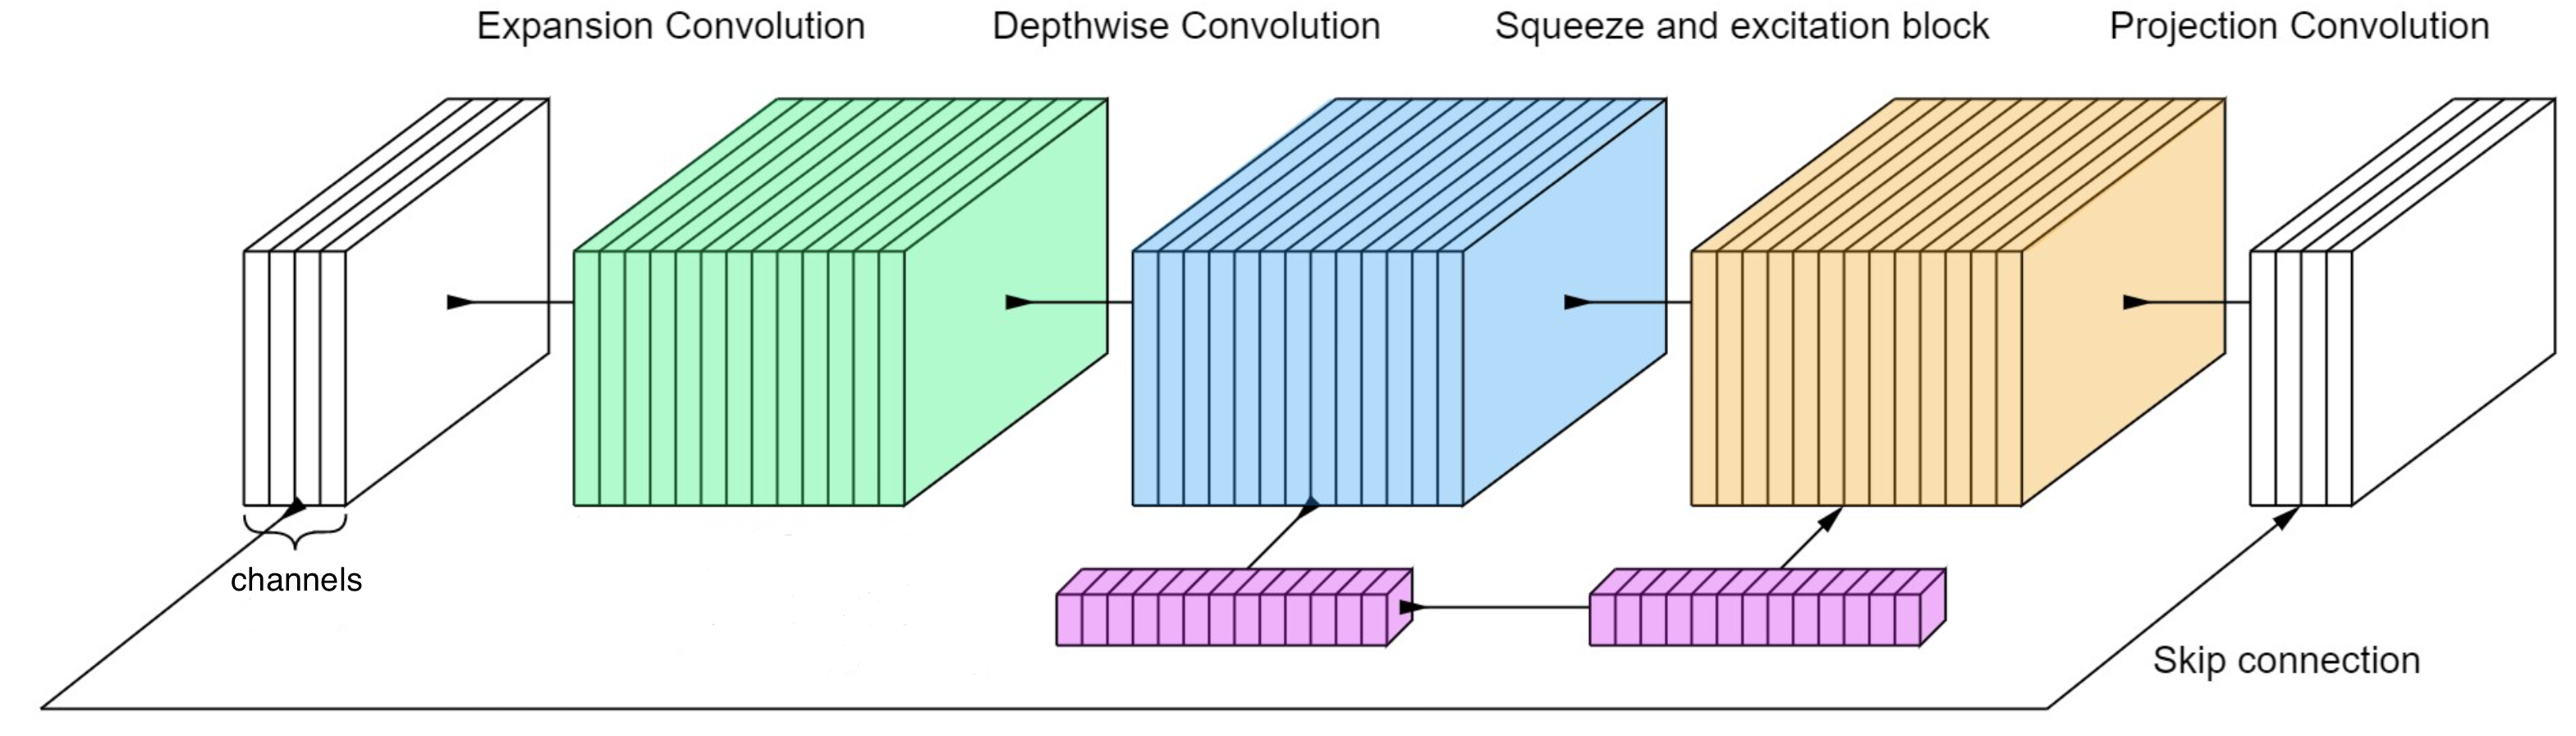
\psfig{file=immagini/convblock.png,width=0.75\textwidth}
    \caption{\textit{Blocco convoluzionale delle PhiNets}. Il numero di canali viene innanzitutto aumentato con una convoluzione pointwise, seguita da una convoluzione depthwise e un blocco di \textit{squeeze and excitation}. Infine, una seconda convoluzione pointwise si collega al blocco di output a bassa dimensionalità.}
    \label{fig:phinetsconvblock}
\end{figure}

\subsection{Fattori di scala}
Come ampiamente anticipato, le architetture progettate per l'inferenza di modelli di machine learining su dispositivi con capacità limitate adottano l'utilizzo di determinati fattori di scala, anche detti \textit{iperparametri}, per adattare la struttura e il consumo di risorse della rete alla specifica piattaforma utilizzata.

In particolare la famiglia delle PhiNets utilizza 4 differenti iperparametri che modificano l'architettura della rete:

\begin{itemize}
    \item $\alpha$: detto \textit{width factor}, regola la larghezza della rete cambiando il numero di canali in uscita da ogni layer;
    \item $\beta$: detto \textit{shape factor}, modifica la risoluzione spaziale delle immagini in ingresso a ogni strato convolutivo;
    \item $t_{0}$: detto \textit{base expansion factor}, regola il numero di canali delle rappresentazioni espanse durante l'esecuzione ogni blocco residuale invertito, in particolare il fattore di espansione varia linearmente con la profondità della rete seguendo la legge $t = t_{o}\left( \frac{(\beta-1)n + N}{N} \right)$, in cui $n$ è l'indice del blocco convolutivo a cui si fa riferimento;
    \item $N$: è il numero di layers totale della rete e ne modifica quindi la profondità.
\end{itemize}

La variazione di ogni singolo parametro ha effetti differenti sulla struttura del modello e sull'impiego di risorse; nello specifico sono metriche di interesse il numero di operazioni per l'inferenza, che determina il consumo di potenza del dispositivo, e il numero totale di parametri della rete, che ne stabilisce l'occupazione di memoria.

Il numero di operazioni totali per l'esecuzione del modello dipende dalla risoluzione $w \times h$ dell'immagine in ingresso, dalla profondità della rete ($N$) e dalla sua larghezza, che scala quadraticamente rispetto al fattore $\alpha$. 
Il numero di parametri è invece determinato dalla dimensione dei kernel dei blocchi convolutivi della rete, che aumenta linearmente con la sua profondità $N$ e col fattore $\beta$.

\section{Obiettivo di ricerca}
\label{sec:ricerca}

Tra le difficoltà relative l'utilizzo di architetture flessibili su determinate piattaforme è di particolare rilevanza quella di individuare l'insieme dei fattori di scala che definiscono una rete compatibile con le risorse del dispositivo sulla quale si vuole operare. 
Parlando quindi delle PhiNets, ci sono molteplici combinazioni degli iperaparametri \textit{$\alpha$, $\beta$, $t_{0}$, $N$} che soddisfano un determinato vincolo di capacità di memoria e che sarebbero quindi adatte all'utilizzo, tuttavia ognuna di queste configurazioni avrà prestazioni di classificazione differenti.

Tale ricerca ha quindi lo scopo di fornire delle logiche per l'individuazione dell'insieme dei fattori di scala che definiscono una PhiNet con le performance migliori per un determinato budget di risorse computazionali.

Nello specifico con ``risorse computazionali" si intendono l'occupazione della memoria FLASH del modello, che è definita dal numero di parametri totali della rete, l'utilizzo della memoria RAM, che nel caso delle PhiNet è determinata dalla dimensione dei tensori nelle operazioni di espansione del primo blocco convoluzionale, e il consumo di energia, che dipende dal numero di operazioni necessarie per eseguire un'inferenza del modello.

Nel corso di questa analisi assume particolare importanza lo studio del numero di layer $N$ della rete che massimizza l'accuratezza di classificazione per determinati intervalli di spazio di archiviazione disponibile; questo è dovuto al fatto che, una volta trovato tale valore per un certo budget di memoria FLASH, rimangono da regolare 3 diversi iperaparametri con a disposizione 3 vincoli (FLASH, RAM, operazioni) e ciò è facilmente risolvibile tramite un sistema a triplice incognita.

Per poter condurre questo tipo di ricerca sarebbe conveniente uno strumento che consenta di determinare l'accuratezza di classificazione di una rete convoluzionale, in particolare di una PhiNet, conoscendo la caratteristiche del modello, definite dagli iperparametri scelti. Dato che le variabili in gioco sono molto complesse e che non è possibile fornire un risultato esatto di tale metrica, diventa utile lo sviluppo di modelli di regressione che approssimino con precisione l'accuratezza di classificazione di una rete.

\iffalse
SCALETTA
\begin{itemize}
    \item problema
    \item obiettivo
    \item concentro su numero di layer 
    \item perche
\end{itemize}
\fi


\section{Raccolta dati}
\label{sec:dati}

A questo scopo si rende necessaria la raccolta di una quantità considerevole di dati riguardanti le performance rispetto alle caratteristiche del modello, in particolare per poter individuare una tendenza dei dati riguardanti il numero di layer dell'architettura è rilevante osservare l'andamento dell'accuratezza di classificazione rispetto al numero di parametri totali delle reti.

Questi dati sono ottenibili solamente tramite l'addestramento di molteplici PhiNets con diverse caratteristiche e l'estrazione del numero totale di parametri e dell'accuratezza di classificazione sul dataset di test per ottenere le reali prestazioni. Naturalmente, per poter rendere l'analisi il più efficace possibile, le configurazioni di rete generate dovrebbero coprire uniformemente l'intervallo di dati (numero di parametri) di interesse, definito a priori.

Per le piattaforme embedded più popolari la quantità di memoria FLASH disponibile è molto limitata, si parla infatti di uno spazio di archiviazione nell'ordine di grandezza dei KB o MB. Per esempio il dispositivo \textit{Arduino UNO ATmega328P} dispone di 32KB di memoria FLASH, la scheda $UC32$ ne possiede 512KB, $STM32L476$ ne ha disponibile 1MB, $STM32H7$ e $MSP432P411$ hanno uno spazio di archiviazione di 2MB, mentre dispositivi come il \textit{Raspberry Pi 3 B+} concedono un flessibilità maggiore dato che dispongono di un ingresso per una scheda SD esterna di parecchi MB.

Considerando quindi che ogni parametro di una PhiNet implementata per piattaforme embedded occupa 8 bit di memoria, è immediato osservare che il possibile intervallo di interesse, che copra anche i casi limite, spazi da $10^{4}$ a $10^{7}$ parametri di rete.

Dato che si tratta di un range molto ampio e data la natura esponenziale degli ordini di grandezza nel mondo informatico, avrebbe poco senso una distribuzione di dati linearmente omogenea, assume invece una grande rilevanza una disposizione ed una visualizzazione dei dati in scala logaritmica, come mostrato in figura \ref{fig:dati}.

L'obiettivo principale diventa quindi l'inizializzazione e l'addestramento di PhiNets che siano adeguatamente distribuite all'interno di questo range logaritmico e per fare ciò è necessario definire uno spazio di ricerca degli iperparametri che soddisfi queste condizioni. 

Le reti addestrate sono oltre 250, il loro numero di parametri copre in maniera omogenea l'intervallo scelto e per ottenerle sono state selezionate diverse combinazioni degli iperparametri \textit{$\alpha$, $\beta$, $t_{0}$, $N$} in maniera tale che il valore di ogni fattore fosse ragionevole e adatto al contesto di utilizzo di questo tipo di reti e che i modelli generati mantenessero una determinata coerenza di struttura.
In particolare il fattore di larghezza $\alpha$ può assumere 5 differenti valori rappresentati in questo insieme $[0.15, 0.3, 0.5, 0.9, 1.5]$, il fattore di forma $\beta$ varia tra $[0.75, 1.05, 1.35]$, il fattore di espansione di base $t_{0}$ viene scelto tra $[4, 5, 6]$, mentre il numero di strti convolutivi $N$ può assumere 6 valori, ovvero $[4, 5, 6, 7, 8, 9]$.

% DA METTERE LA TABELLA?
\iffalse
\begin{center}
    \begin{tabular}{|c|c|}
        \hline
        Fattore di scala & \multicolumn{1}{c|}{Valori} \\
        \hline
        $\alpha$ & $0.15, 0.3, 0.5, 0.9, 1.5$ \\
        $\beta$ & $0.75, 1.05, 1.35$ \\
        $t_{0}$ & $4, 5, 6$ \\
        $N$ & $4, 5, 6, 7, 8, 9$ \\
        \hline
    \end{tabular}
\end{center}
\fi

Tramite le varie permutazioni lungo questo spazio di iperparametri si ottengono quindi configurazioni di PhiNets differenti che sono caratterizzate, oltre che da una diversa struttura di rete, da un numero di parametri totali differente e da una diversa accuratezza nella classificazione di immagini.

\begin{figure}[ht]
    \centering
    \subfloat[]{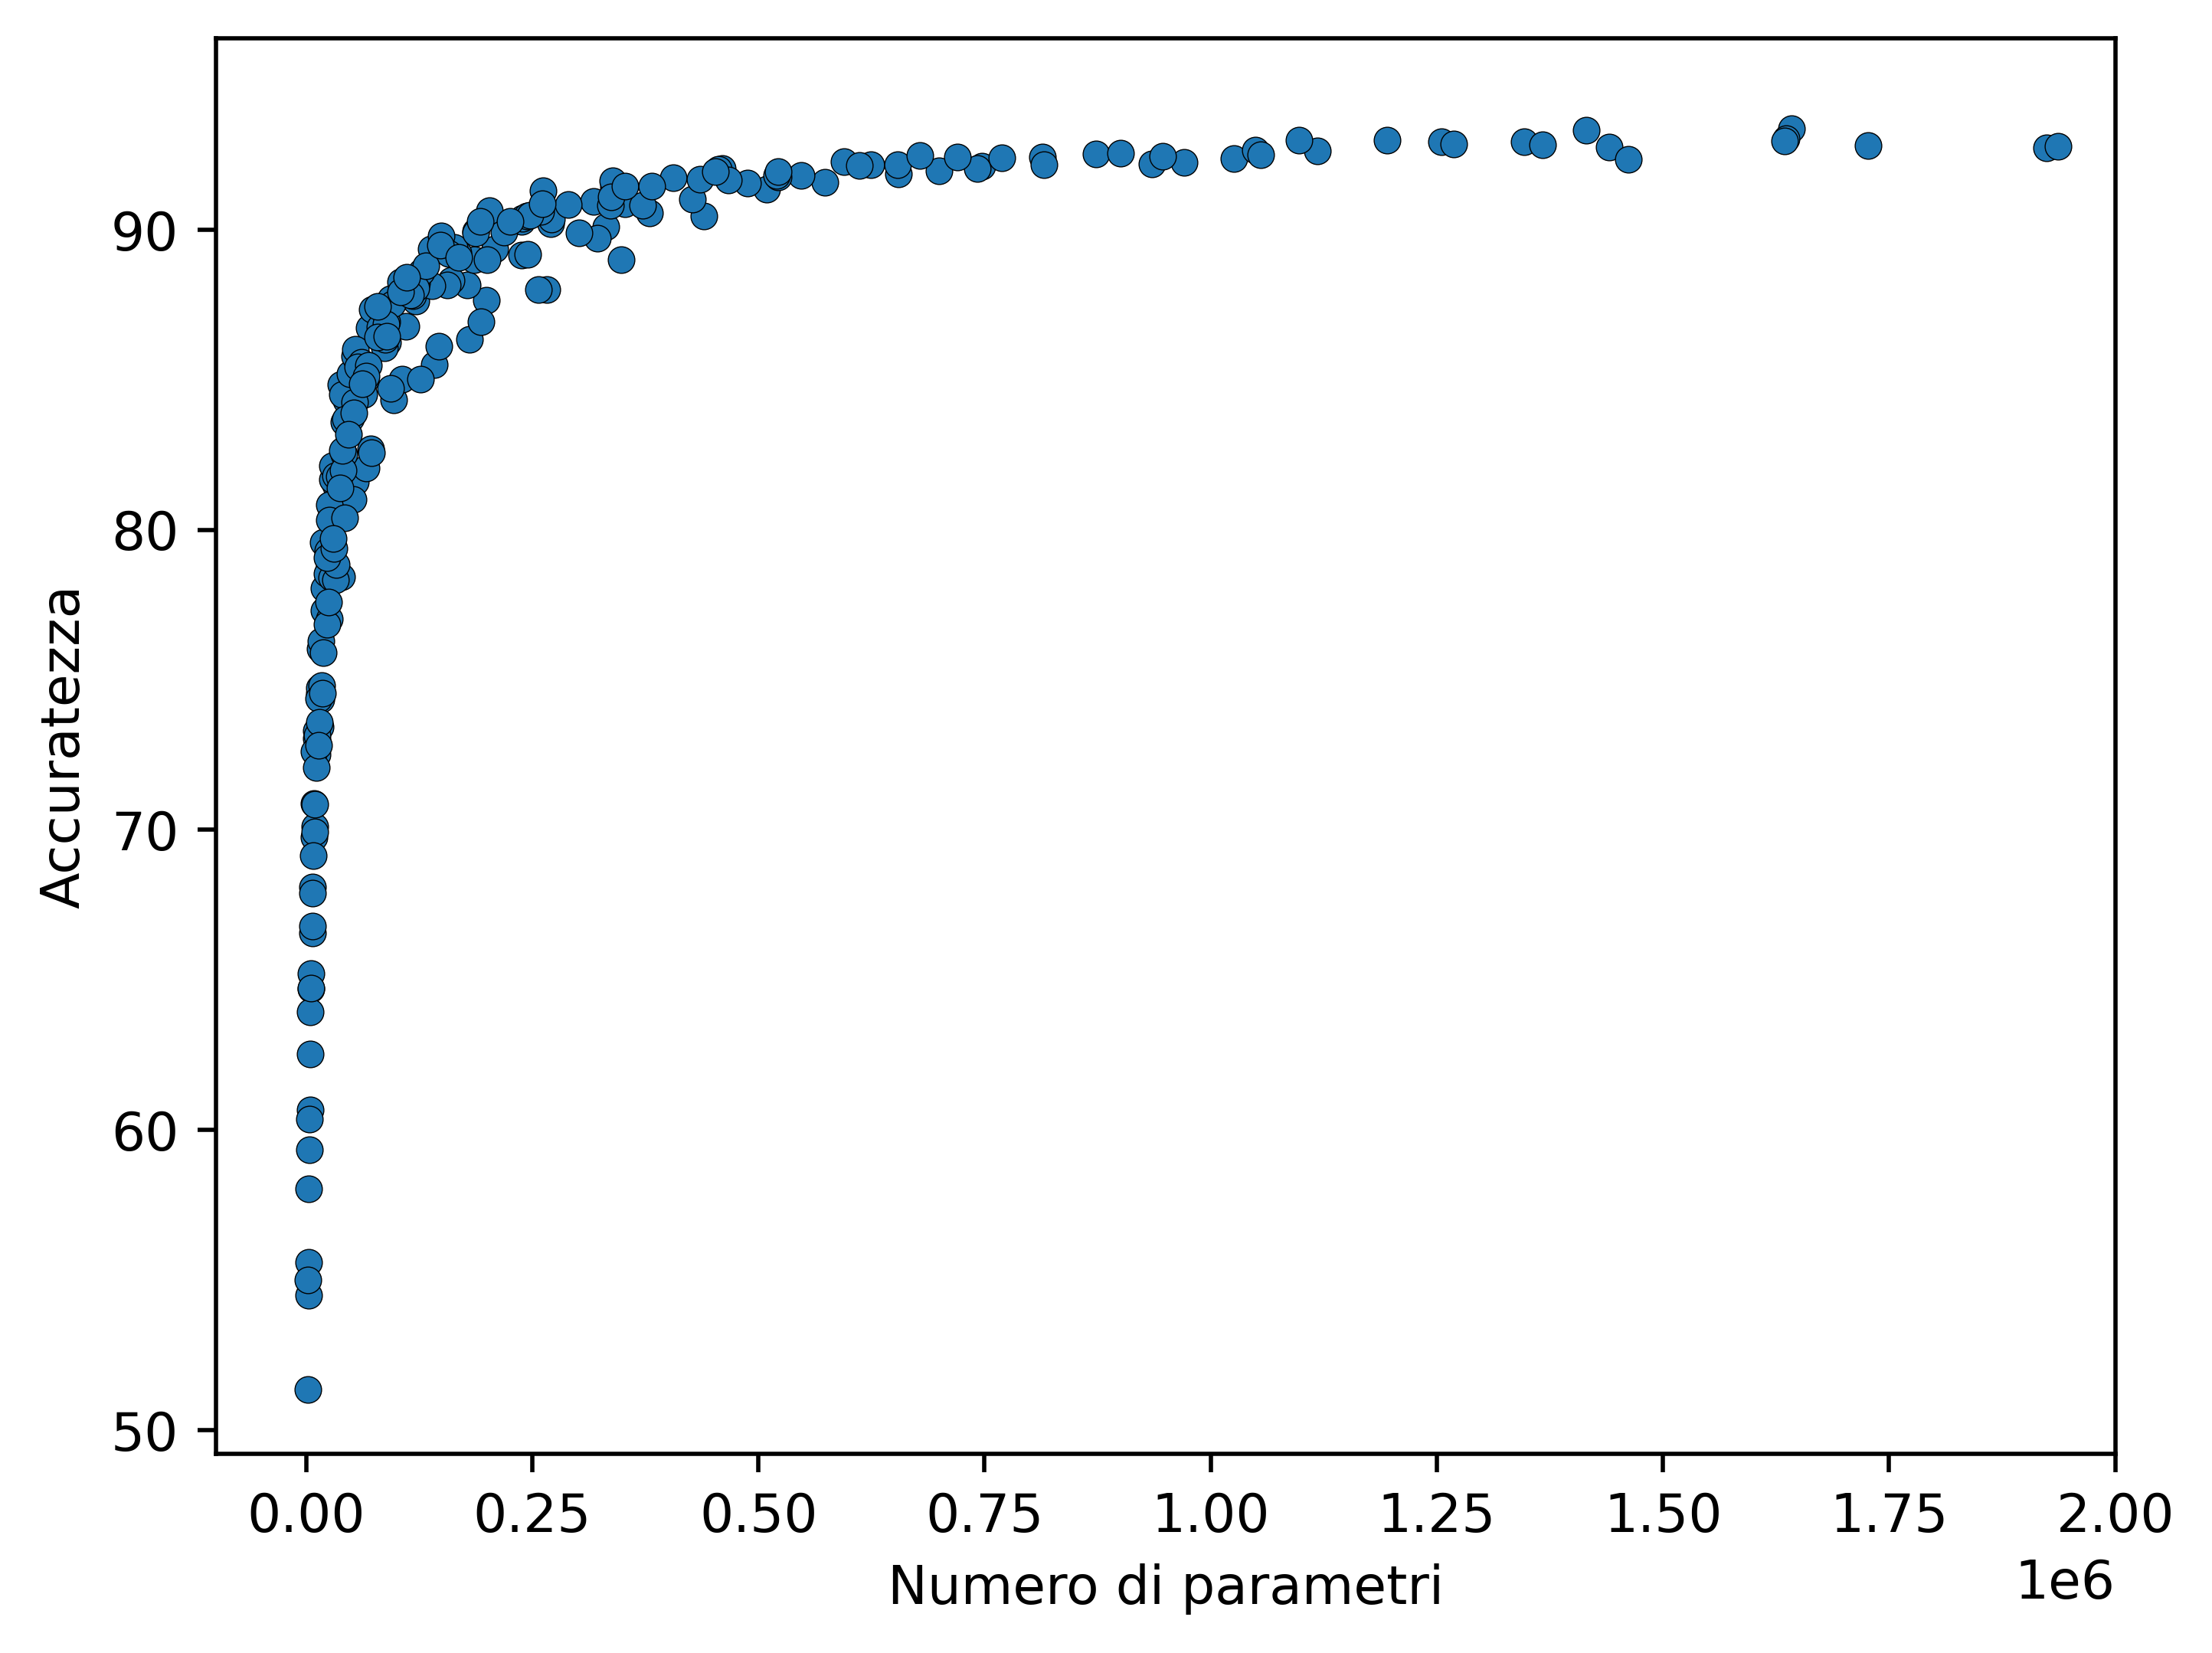
\includegraphics[width=0.4\textwidth]{tesi/immagini/dati_lin.png}}\quad
    \subfloat[]{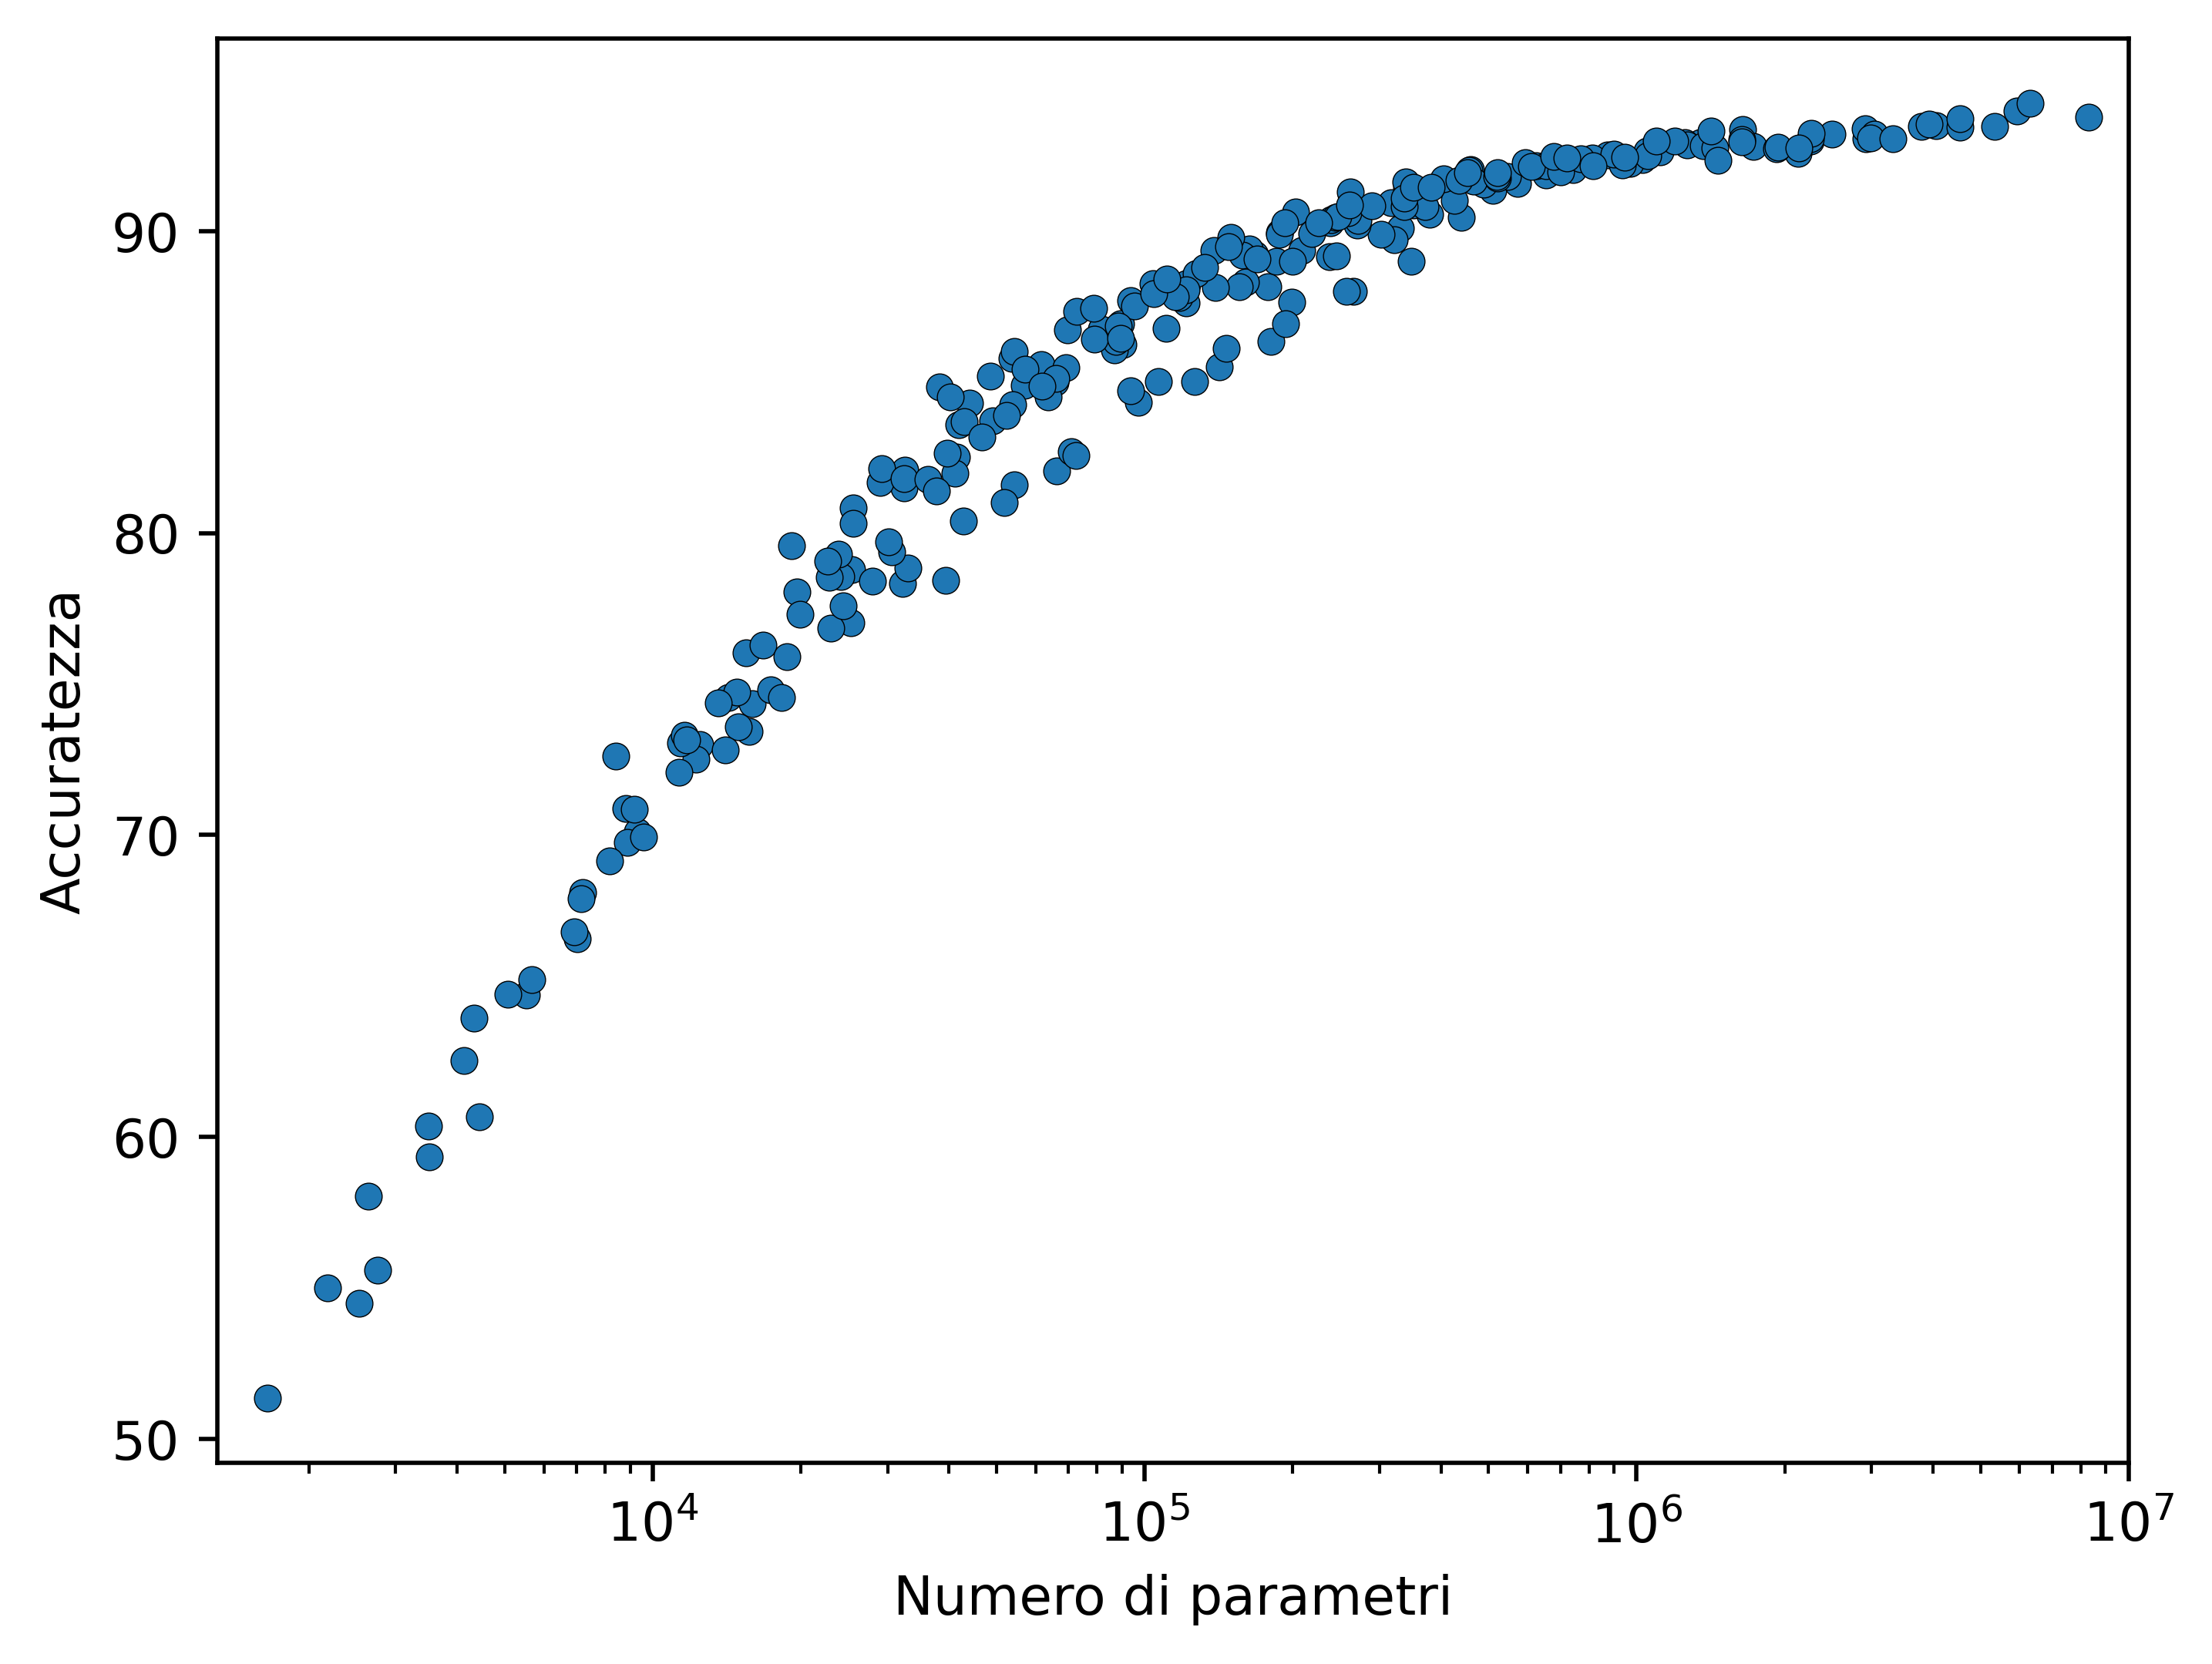
\includegraphics[width=0.4\textwidth]{tesi/immagini/dati_log.png}}\quad
    \caption{\textit{Distribuzione dei dati per l'analisi}. Le due immagini mostrano entrambe la stessa distribuzione di dati, ovvero l'accurateza di classificazione rispetto al numero di parametri di ogni PhiNet. La differenza risiede nella scala, la figura (a) visualizza i dati in scala lineare, (b) li mostra invece in scala logaritmica per una raprresentazione più chiara.}
    \label{fig:dati}
\end{figure}

È importante notare come i dati presentati, ottenuti tramite l'utilizzo degli iperparametri sopra citati, siano omogeneamente distribuiti lungo la scala logaritmica, sottolineando ancora di più la natura esponenziale delle architetture scalabili e l'importanza di visualizzare tali dati nella scala logaritmica durante l'analisi.

\iffalse
SCALETTA
\begin{itemize}
    \item spazio di ricerca numero parametri [..., ...]
    \item scala logaritmica
    \item configurazioni iperparametri
    \item quantità di dati
    \item ...
    \item checkpoint per linear probe
\end{itemize}
\fi


\section{Tecniche di regressione e segmentazione}
% OPPURE ?
%\section{Analisi dati}
\label{sec:regressione}

Come anticipato nella sezione \ref{sec:ricerca}, l'iperparametro delle PhiNets più significativo per lo scopo di ricerca è il numero di strati convolutivi $N$, dato che non sono disponibili logiche o procedure per la scelta ottimale di tale fattore al fine di massimizzare le prestazioni della rete.

A tal proposito è conveniente visualizzare i dati non solo rispetto al numero complessivo dei parametri, ma anche relativamente al numero di layer presenti nel modello al fine di poter scomporre l'analisi per avere dati tra loro più coerenti e facili da visualizzare.


\begin{figure}[ht]
    \centering
    \subfloat[]{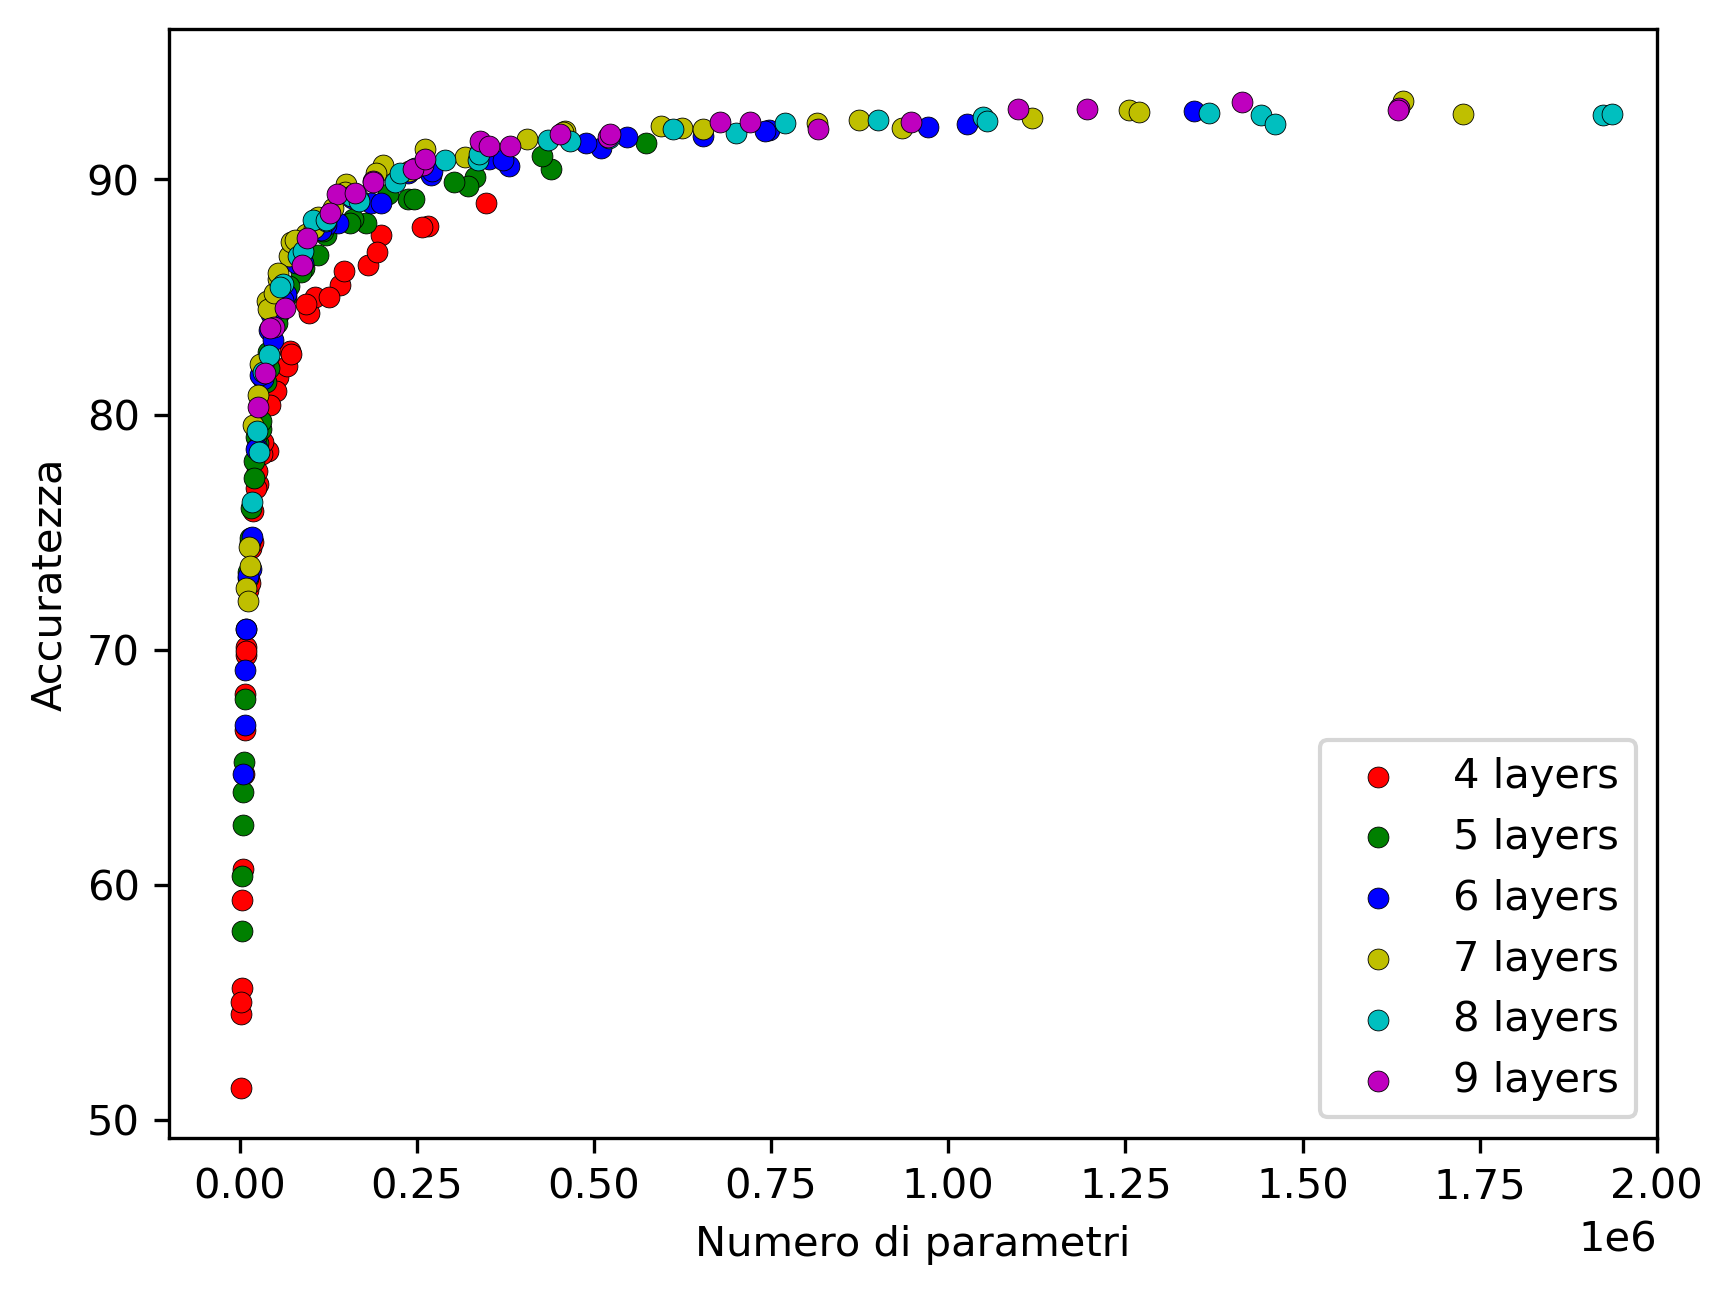
\includegraphics[width=0.4\textwidth]{tesi/immagini/dati_layer_lin.png}}\quad
    \subfloat[]{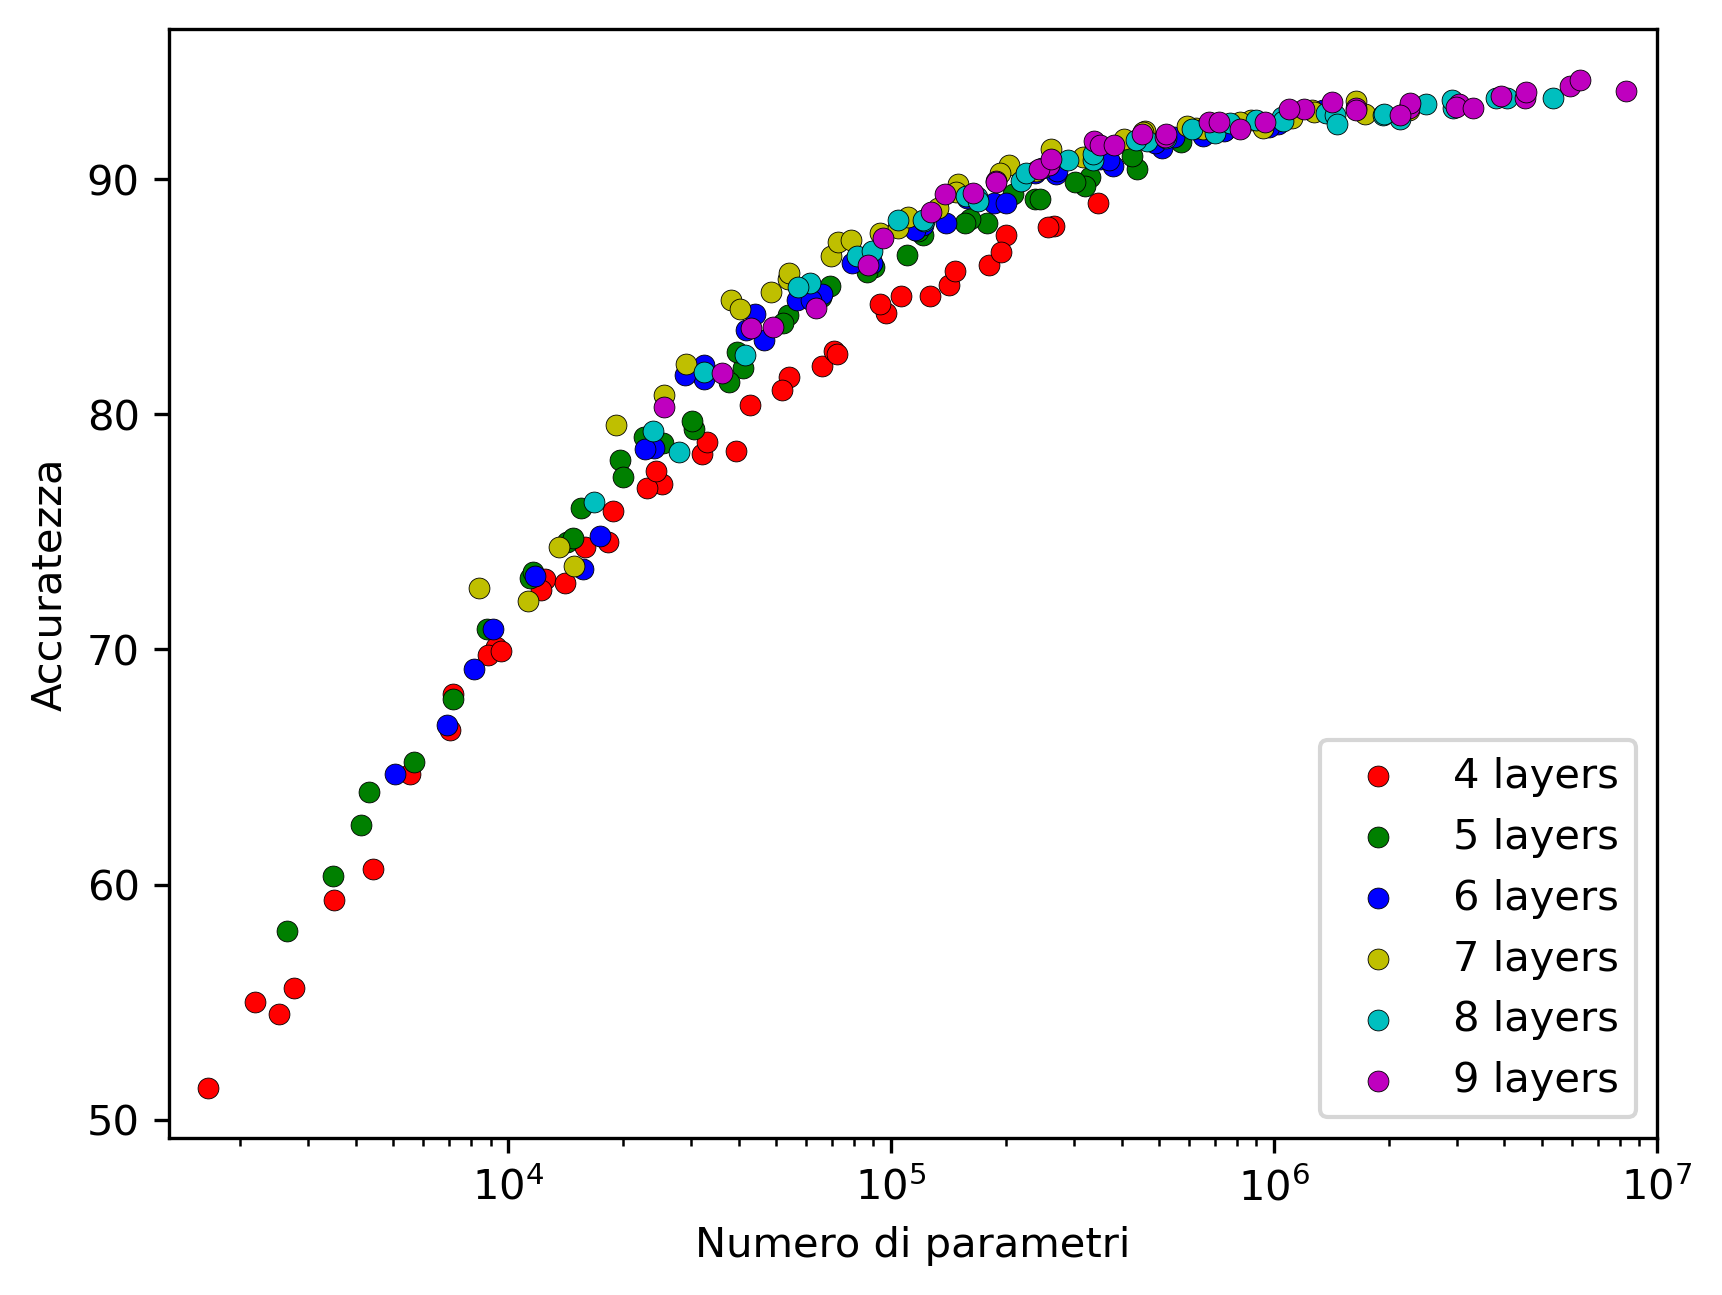
\includegraphics[width=0.4\textwidth]{tesi/immagini/dati_layer_log.png}}\quad
    \caption{\textit{Distribuzione dei dati in base al numero di strati}. I due grafici mostrano gli stessi dati del grafico \ref{fig:dati}, ma è rappresentata anche la dimensione rispetto al numero di layer della rete.}
    \label{fig:dati_layer}
\end{figure}

Come si può osservare qualitativamente in figura \ref{fig:dati_layer}, determinati valori per il fattore $N$ sono spesso da escludere dalla scelta per un determinati budget di memoria FLASH, mentre altri sono da preferire per capacità di numero di parametri più alto. L'intenzione è quindi quella di determinare quantitativamente il numero di strati convoluzionali che ottimizza le performance per ogni possibile valore di capacità di memoria e per fare ciò vengono utilizzate tecniche di regressione e segmentazione dei dati.

I metodi di regressione consentono di approssimare l'andamento di una distribuzione di dati con quello di una funzione e il loro scopo è quello di trovare un modello matematico che descriva al meglio la relazione tra una variabile indipendente (in questo caso il numero di parametri) e una variabile dipendente (in questo caso l'accuratezza di classificazione). Tale processo di regressione coinvolge, oltre la raccolta dei dati, la scelta del modello matematico appropriato, l'adattamento ai dati 
di addestramento e la valutazione delle prestazioni finali tramite determinate metriche, come ad esempio l'errore quadratico medio (MSE).
Le tecniche di segmentazione vengono invece utilizzate per dividere un insieme iniziale di dati in gruppi o segmenti omogenei con determinate caratteristiche, al fine di identificare pattern o tendenze all'interno dei dati.

In questa analisi verranno quindi impiegati sistemi di regressione per approssimare l'andamento dei risultati di classificazione rispetto al numero di parametri per ogni valore differente di numero di strati convolutivi presenti in modo da ottenere un modello matematico adeguatamente preciso per predire e confrontare le prestazioni delle reti; successivamente verranno utilizzati i dati ottenuti con la regressione per segmentare l'intervallo delle ascisse in modo da ottenere determinati range di memoria all'interno dei quali è preferibile scegliere un certo valore del fattore di profondità $N$.

\subsection{Metodi di regressione}

Per trovare la funzione matematica che meglio approssima la distribuzione di dati raccolti, bisogna innanzitutto definire il tipo di andamento che essa deve assumere (può essere lineare, logaritmico, esponenziale ecc.) in funzione di determinati parametri che definiscono i gradi di libertà del modello. Questi parametri sono le incognite che l'algoritmo di ottimizzazione deve trovare tramite il loro aggiustamento, in modo tale da ottenere una bassa discrepanza tra funzione matematica finale ed i dati effettivi disponibili. 

Al fine di ottenere il miglior modello di regressione è necessario provare diversi andamenti e trovare il migliore tramite delle metriche di valutazione dell'errore totale.

\subsubsection{Regressione esponenziale}

Osservando la distribuzione dei dati mostrata in figura \ref{fig:dati_layer} (a) è significativo notare all'interno del grafico la presenza di un asintoto orizzontale verso cui tendono gli andamenti per i diversi valori di $N$. Ciò significa che aumentando il numero di parametri della rete ci si aspetta un'accuratezza di classificazione più elevata che tende al valore stabilito dall'asintoto.

Diventa quindi logico supporre che il modello matematico scelto per approssimare l'andamento corrisponda a una funzione contenente un asintoto orizzontale e una possibile è la funzione esponenziale, in questa situazione modellata con coefficiente negativo secondo la legge:

\begin{equation}
    \centering
    acc = -a^{P - b} + c
\end{equation}

In una funzione matematica di questo tipo \textit{acc} si riferisce all'accuratezza di classificazione, $P$ è il numero totale di parametri della rete e i tre fattori $a$, $b$, $c$ regolano la funzione per adattarsi al meglio alla distribuzione dei dati da modellare. Al crescere del parametro $a$ aumenta la ripidità della curva, mentre i fattori $b$ e $c$ ne controllano la traslazione rispettivamente lungo l'asse delle ascisse e delle ordinate, nello specifico $c$ regola il livello dell'asintoto orizzontale di accuratezza.

\begin{figure}[ht]
    \centering
    \subfloat[]{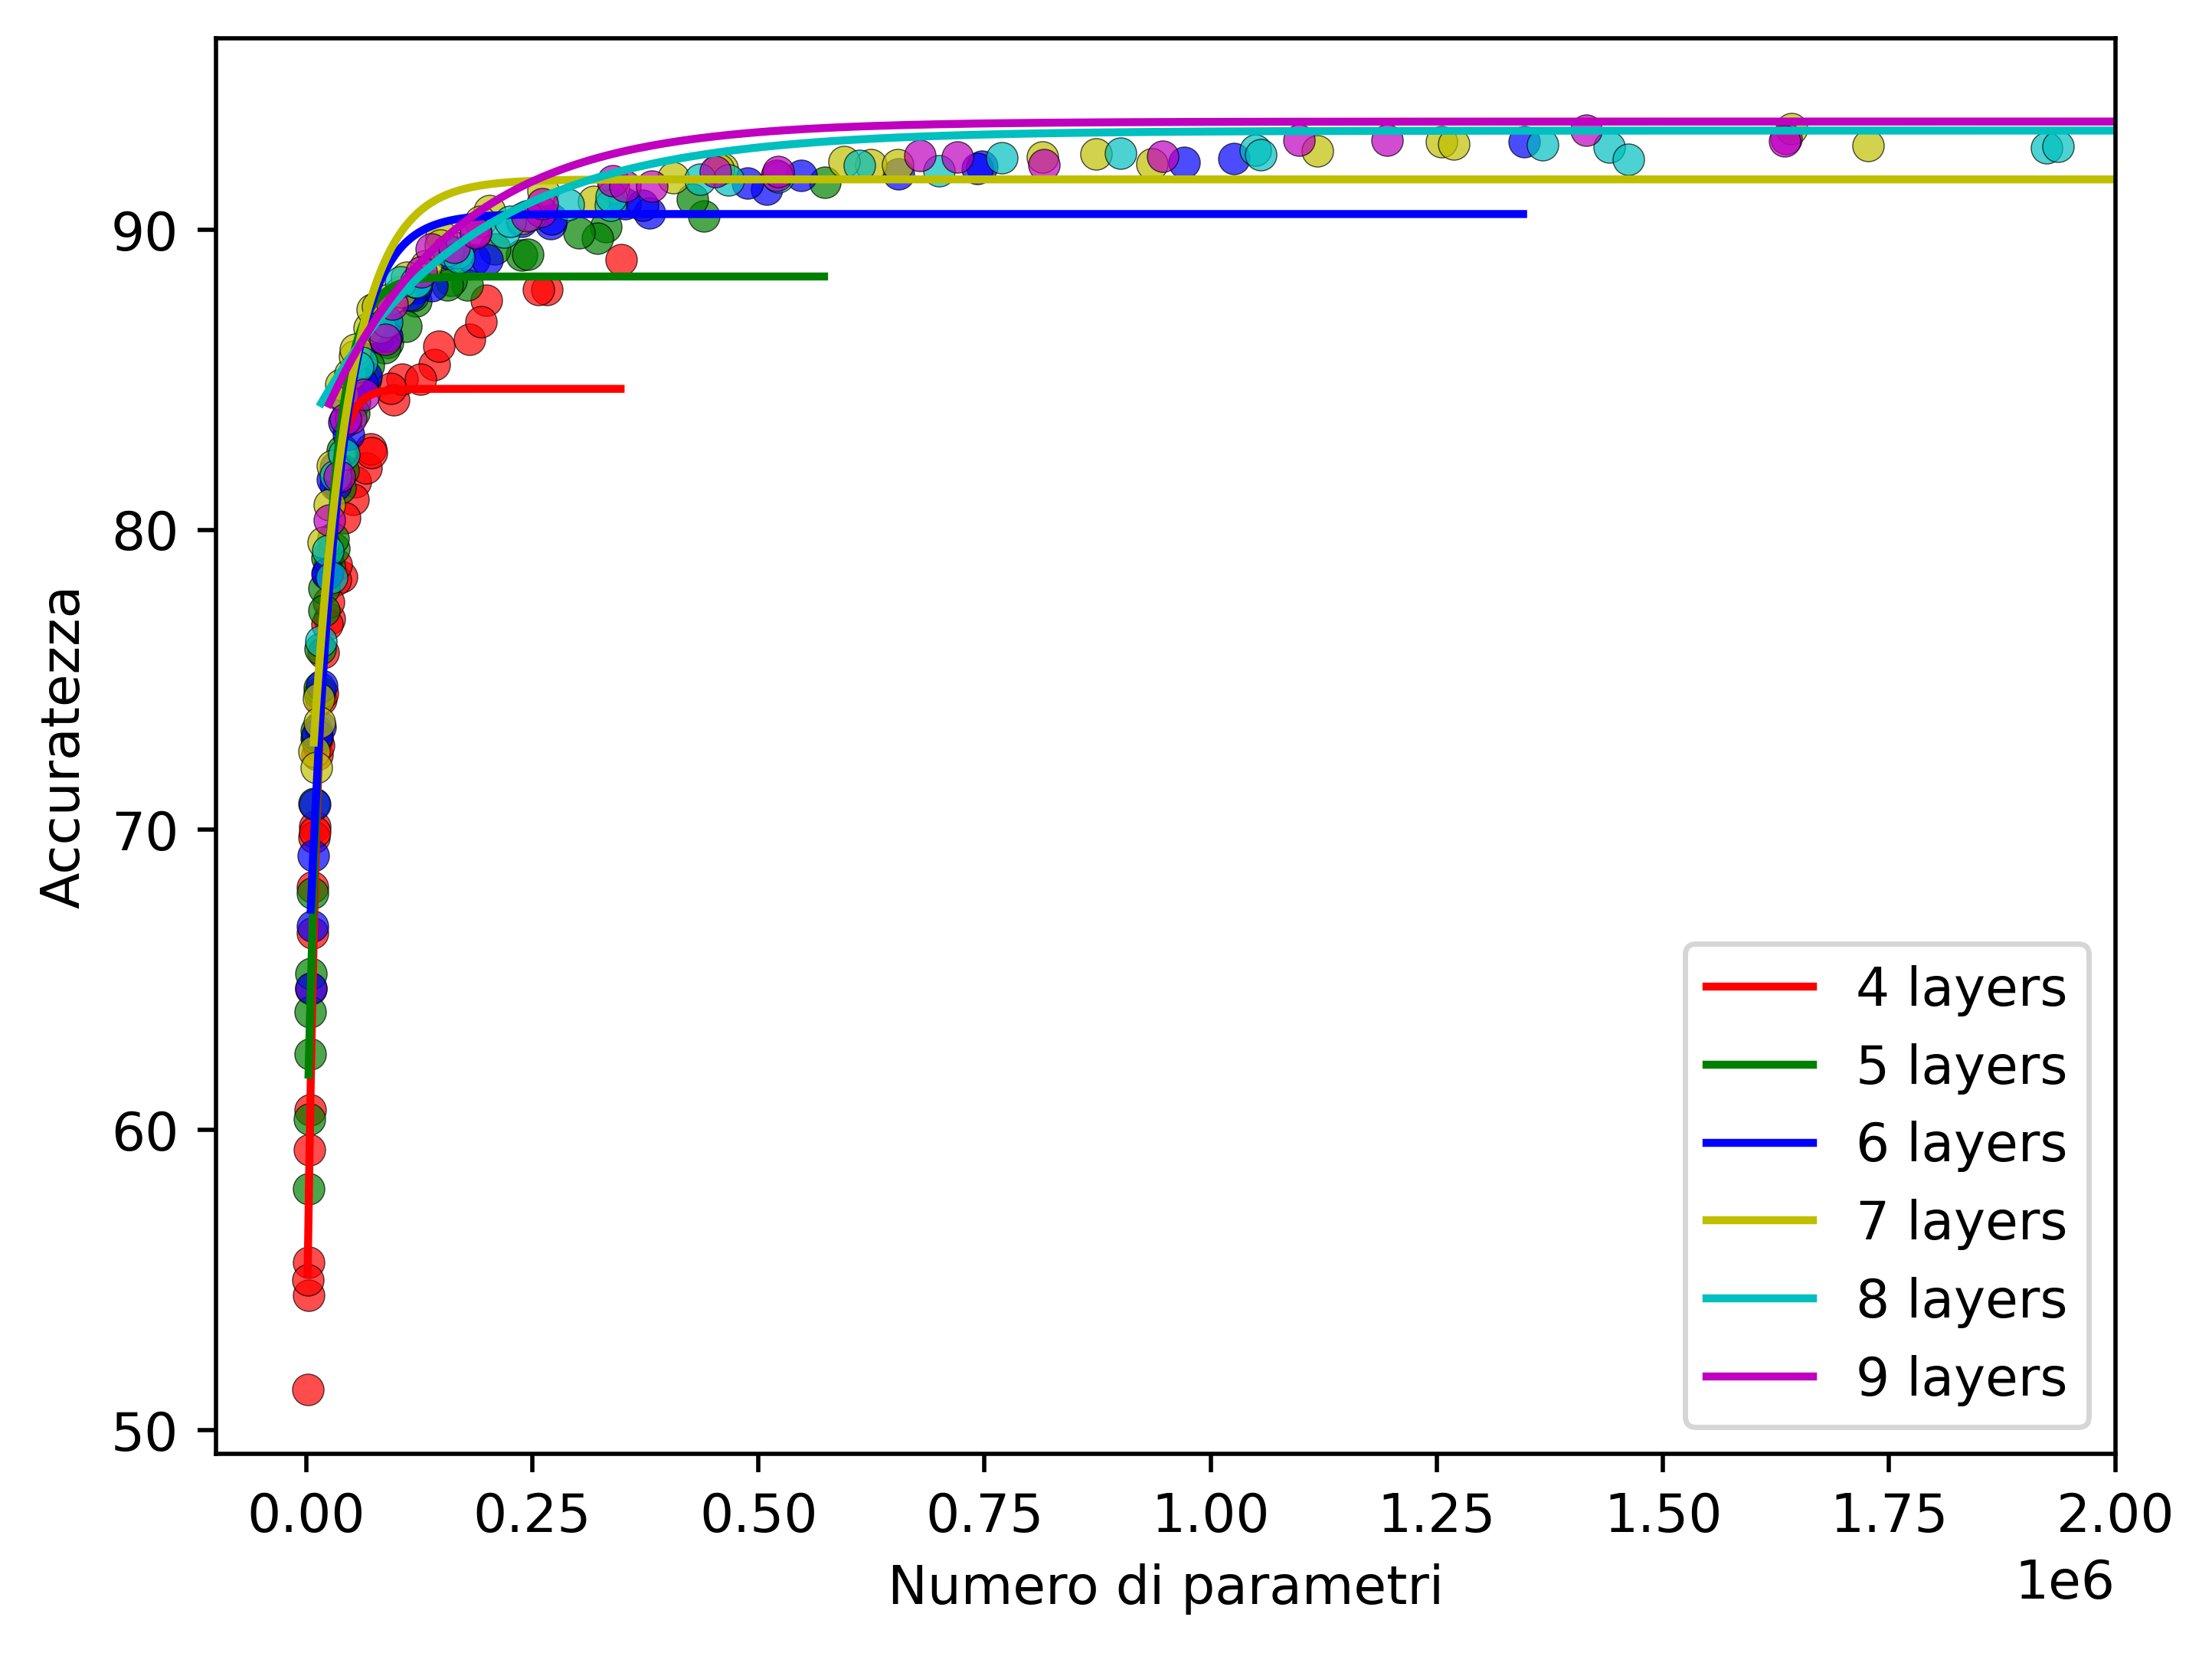
\includegraphics[width=0.4\textwidth]{tesi/immagini/exp_reg.png}}\quad
    \subfloat[]{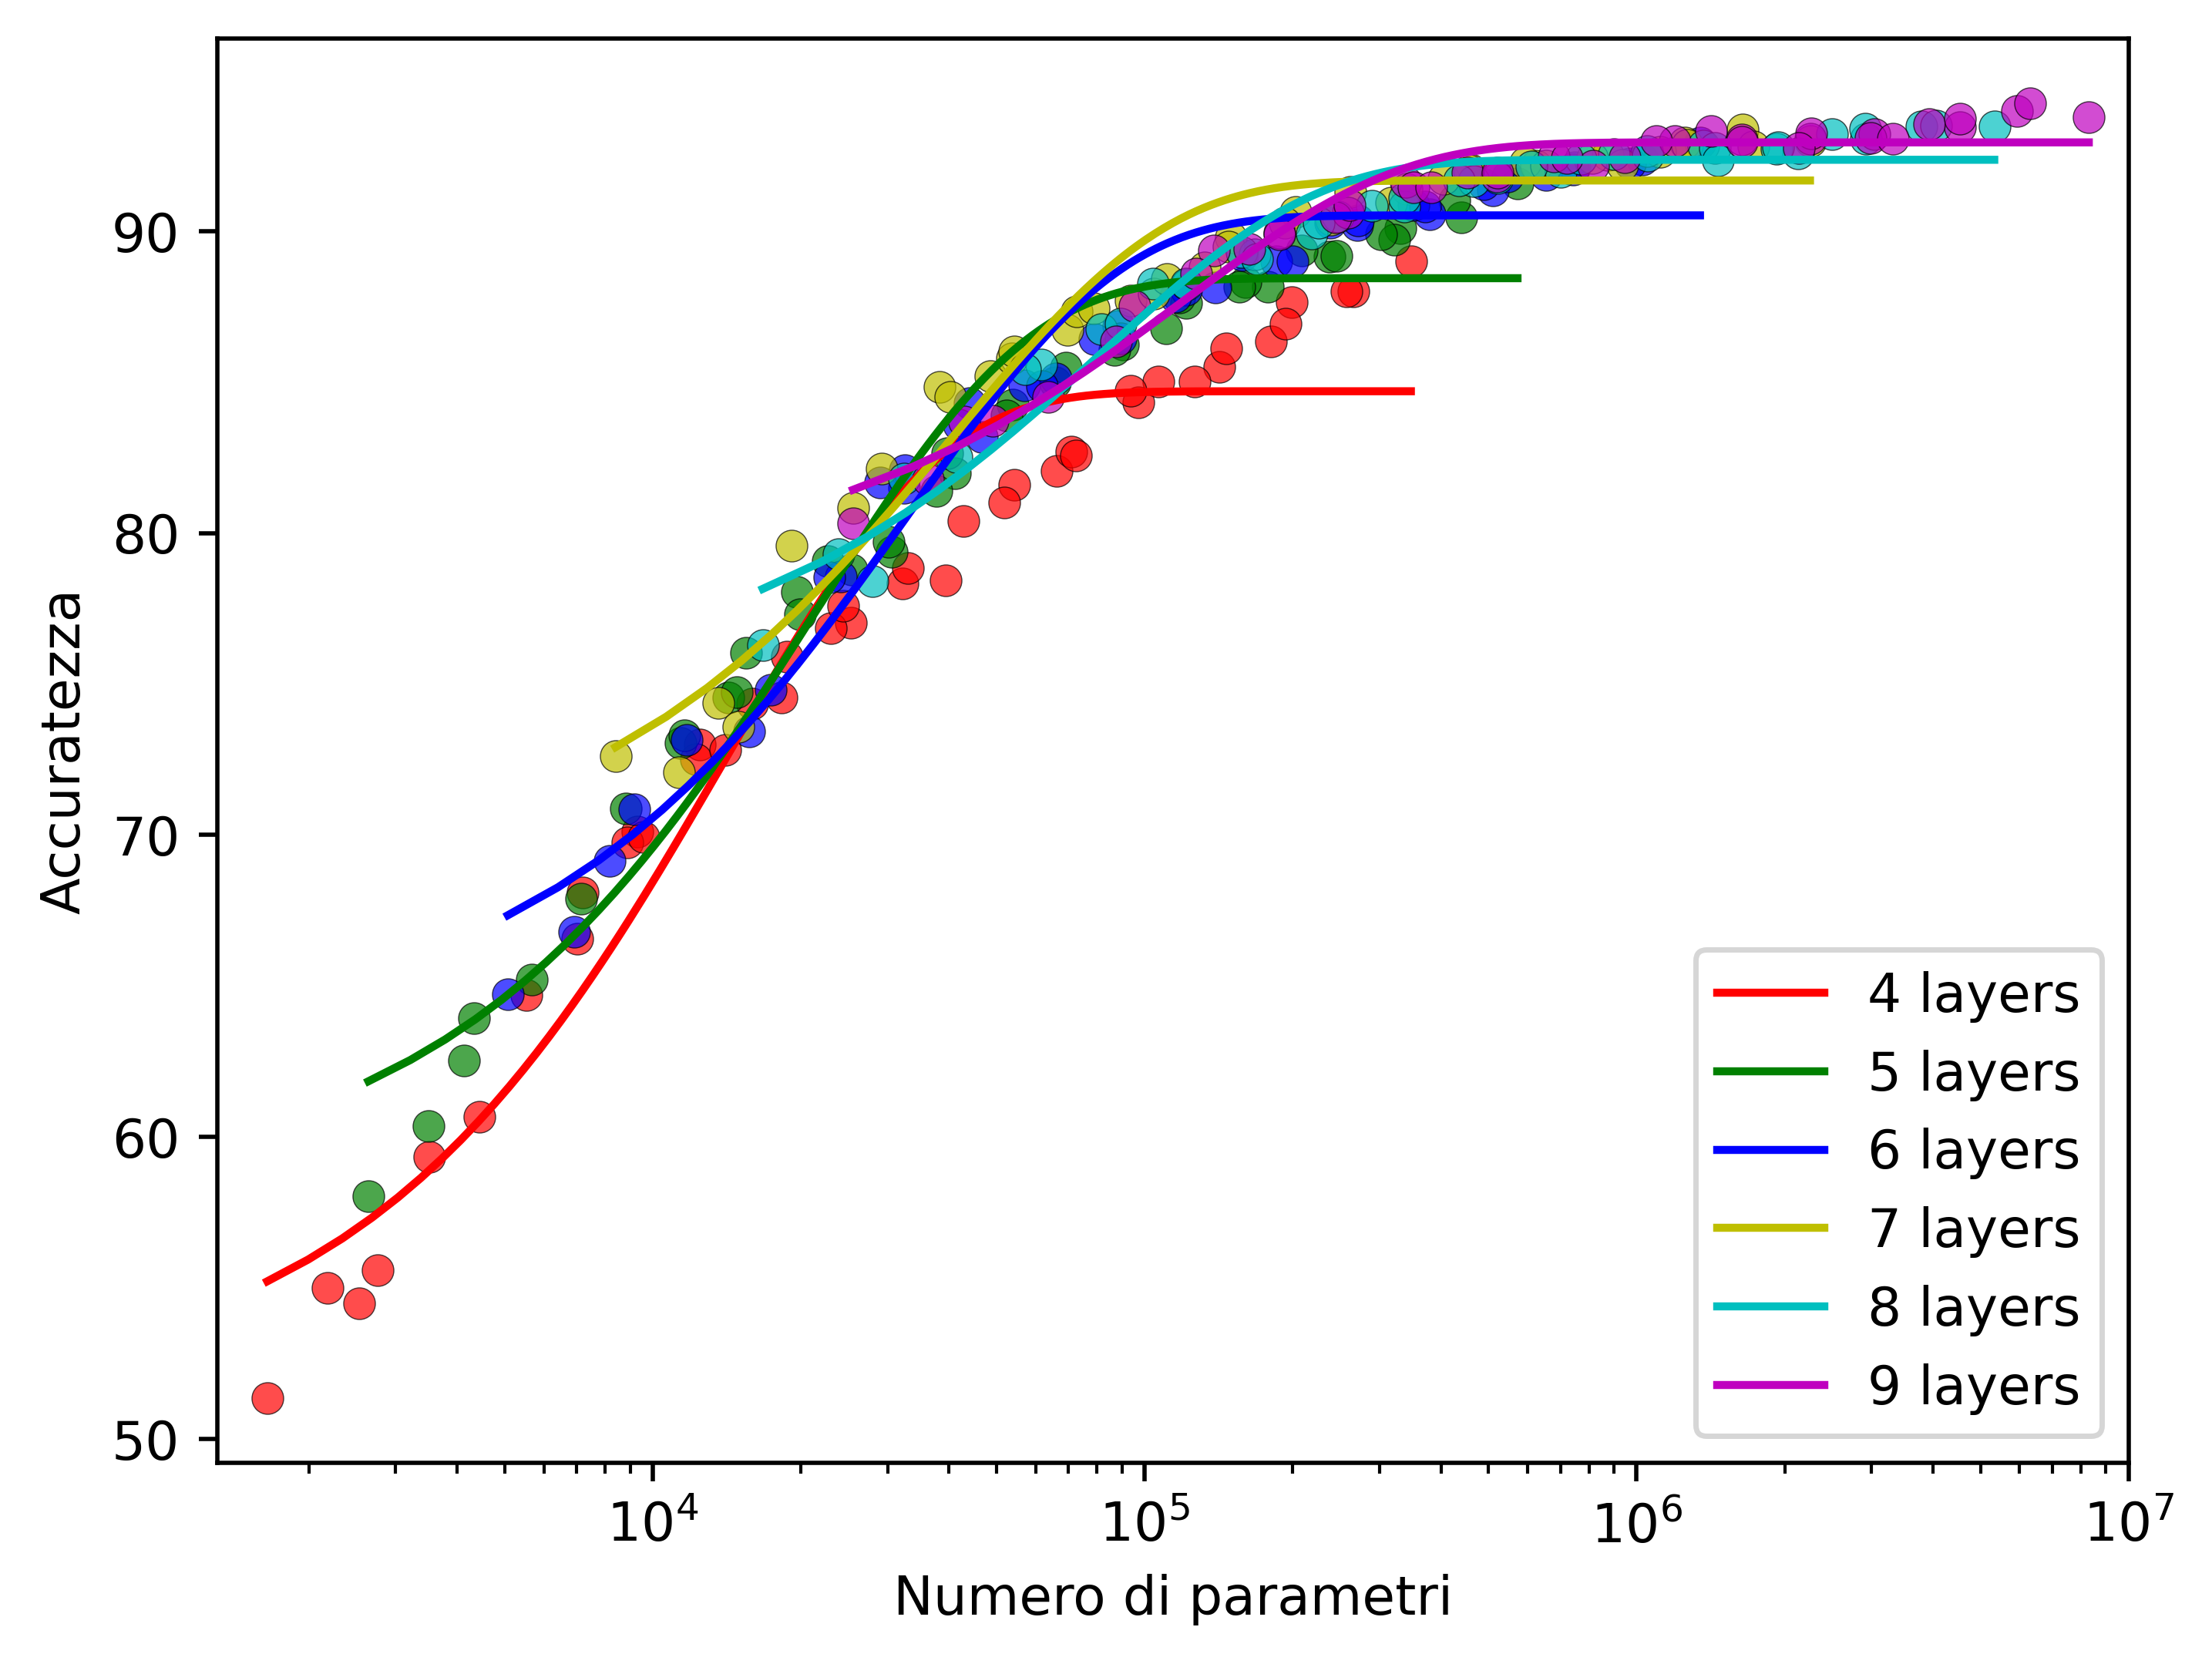
\includegraphics[width=0.4\textwidth]{tesi/immagini/exp_reg_log.png}}\quad
    \caption{\textit{Regressione esponenziale}.}
    \label{fig:exp_reg}
\end{figure}

Come si può notare un modello di regressione esponenziale non è adatto a questo tipo di distribuzione dati in quanto la tendenza della funzione ad appiattirsi sul suo asintoto è troppo marcata e tende ad approssimare meglio i valori intermedi trascurando invece quelli agli estremi dell'intervallo, creando problemi di generalizzazione, infatti per valori elevati di numero di parametri la regressione tende ad approssimare al ribasso l'accuratezza di classificazione facendola tendere al valore $c$. Nella funzione esponenziale è inoltre assente un asintoto verticale che potrebbe rappresentare una possibile soluzione al problema. 

\subsubsection{Regressione logaritmica}

Tra le funzioni che possiedono un asintoto verticale con un andamento monotono decrescente, come nel caso desiderato, è possibile trovare le funzioni logaritmiche che tendono a crescere velocemente nella prima parte della funzione, mantenendo però un incremento significativo per elevati valori dell'asse delle ascisse.

Un possibile modello che possa quindi ricreare l'andamento delle curve logaritmiche è definito dalla relazione:

\begin{equation}
    \centering
    acc = a \cdot log(P - b) + c
\end{equation}

In questa funzione il parametro $a$ regola la rapidità di crescita della curva, i fattori $b$ e $c$ controllano invece le traslazioni dei modelli lungo gli assi cartesiani, in particolare $b$ rappresenta il valore delle ascisse degli asintoti verticali per le diverse configurazioni di layer.

\begin{figure}[ht]
    \centering
    \subfloat[]{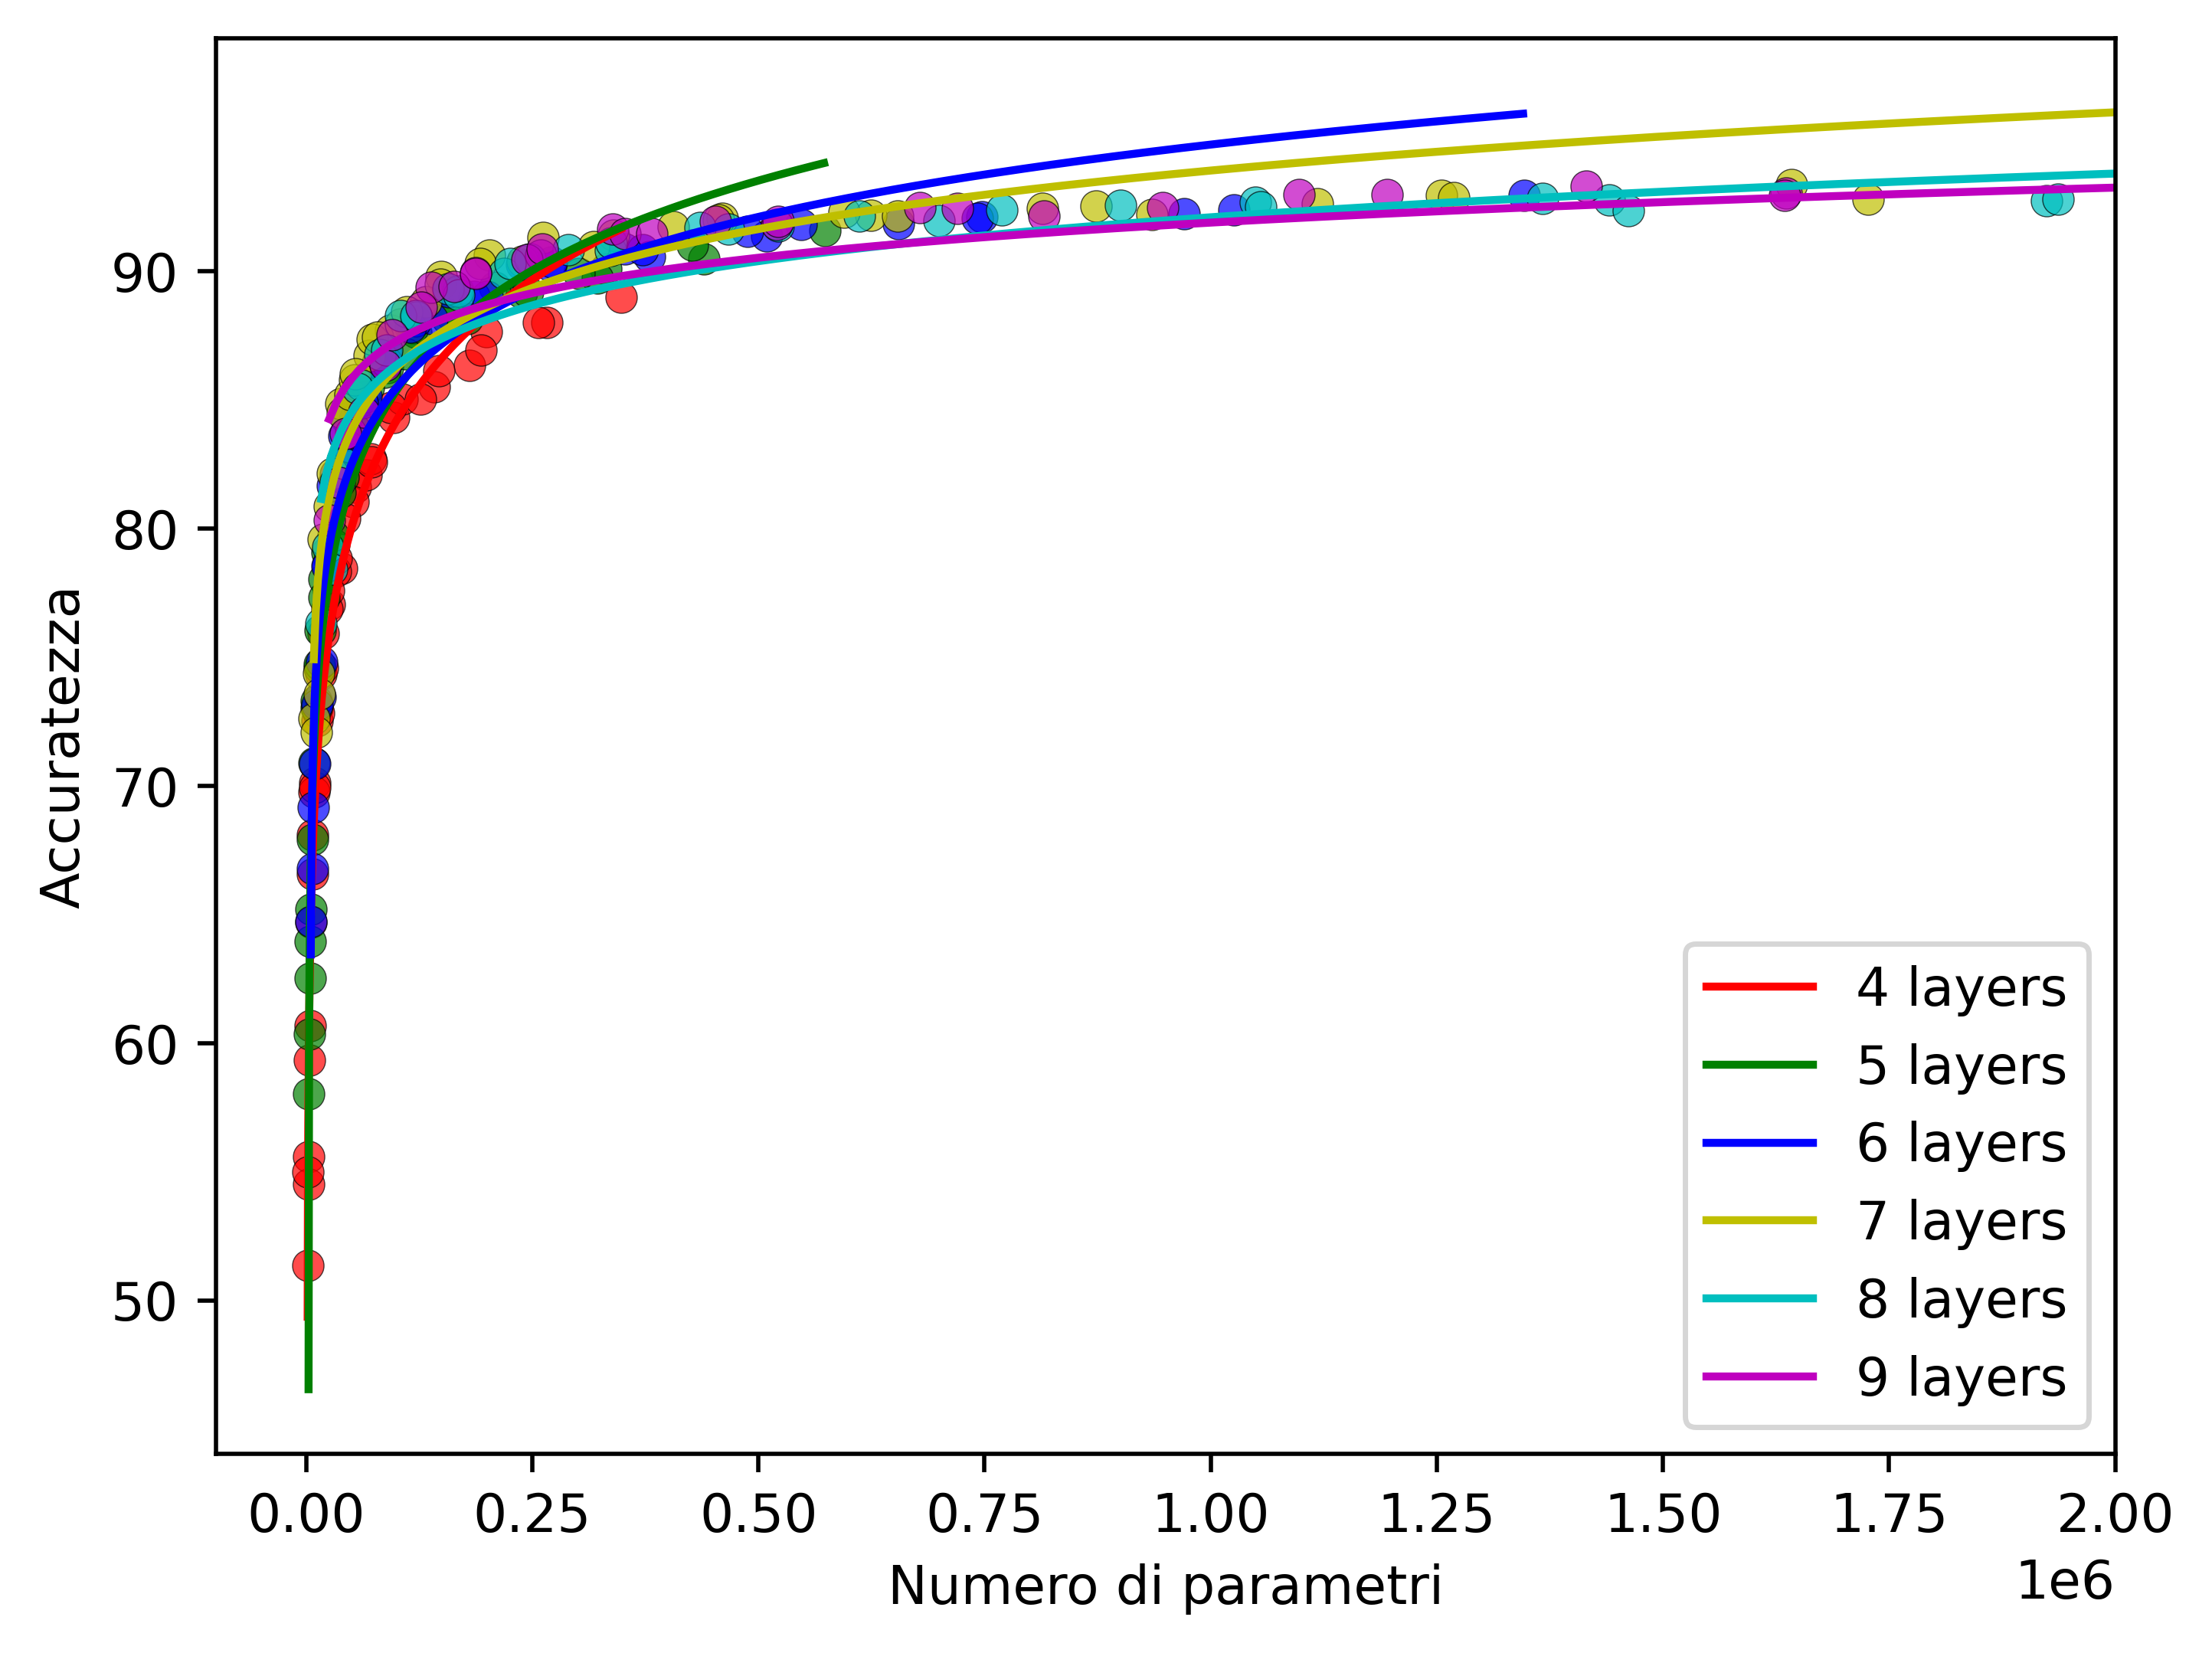
\includegraphics[width=0.4\textwidth]{tesi/immagini/log_reg.png}}\quad
    \subfloat[]{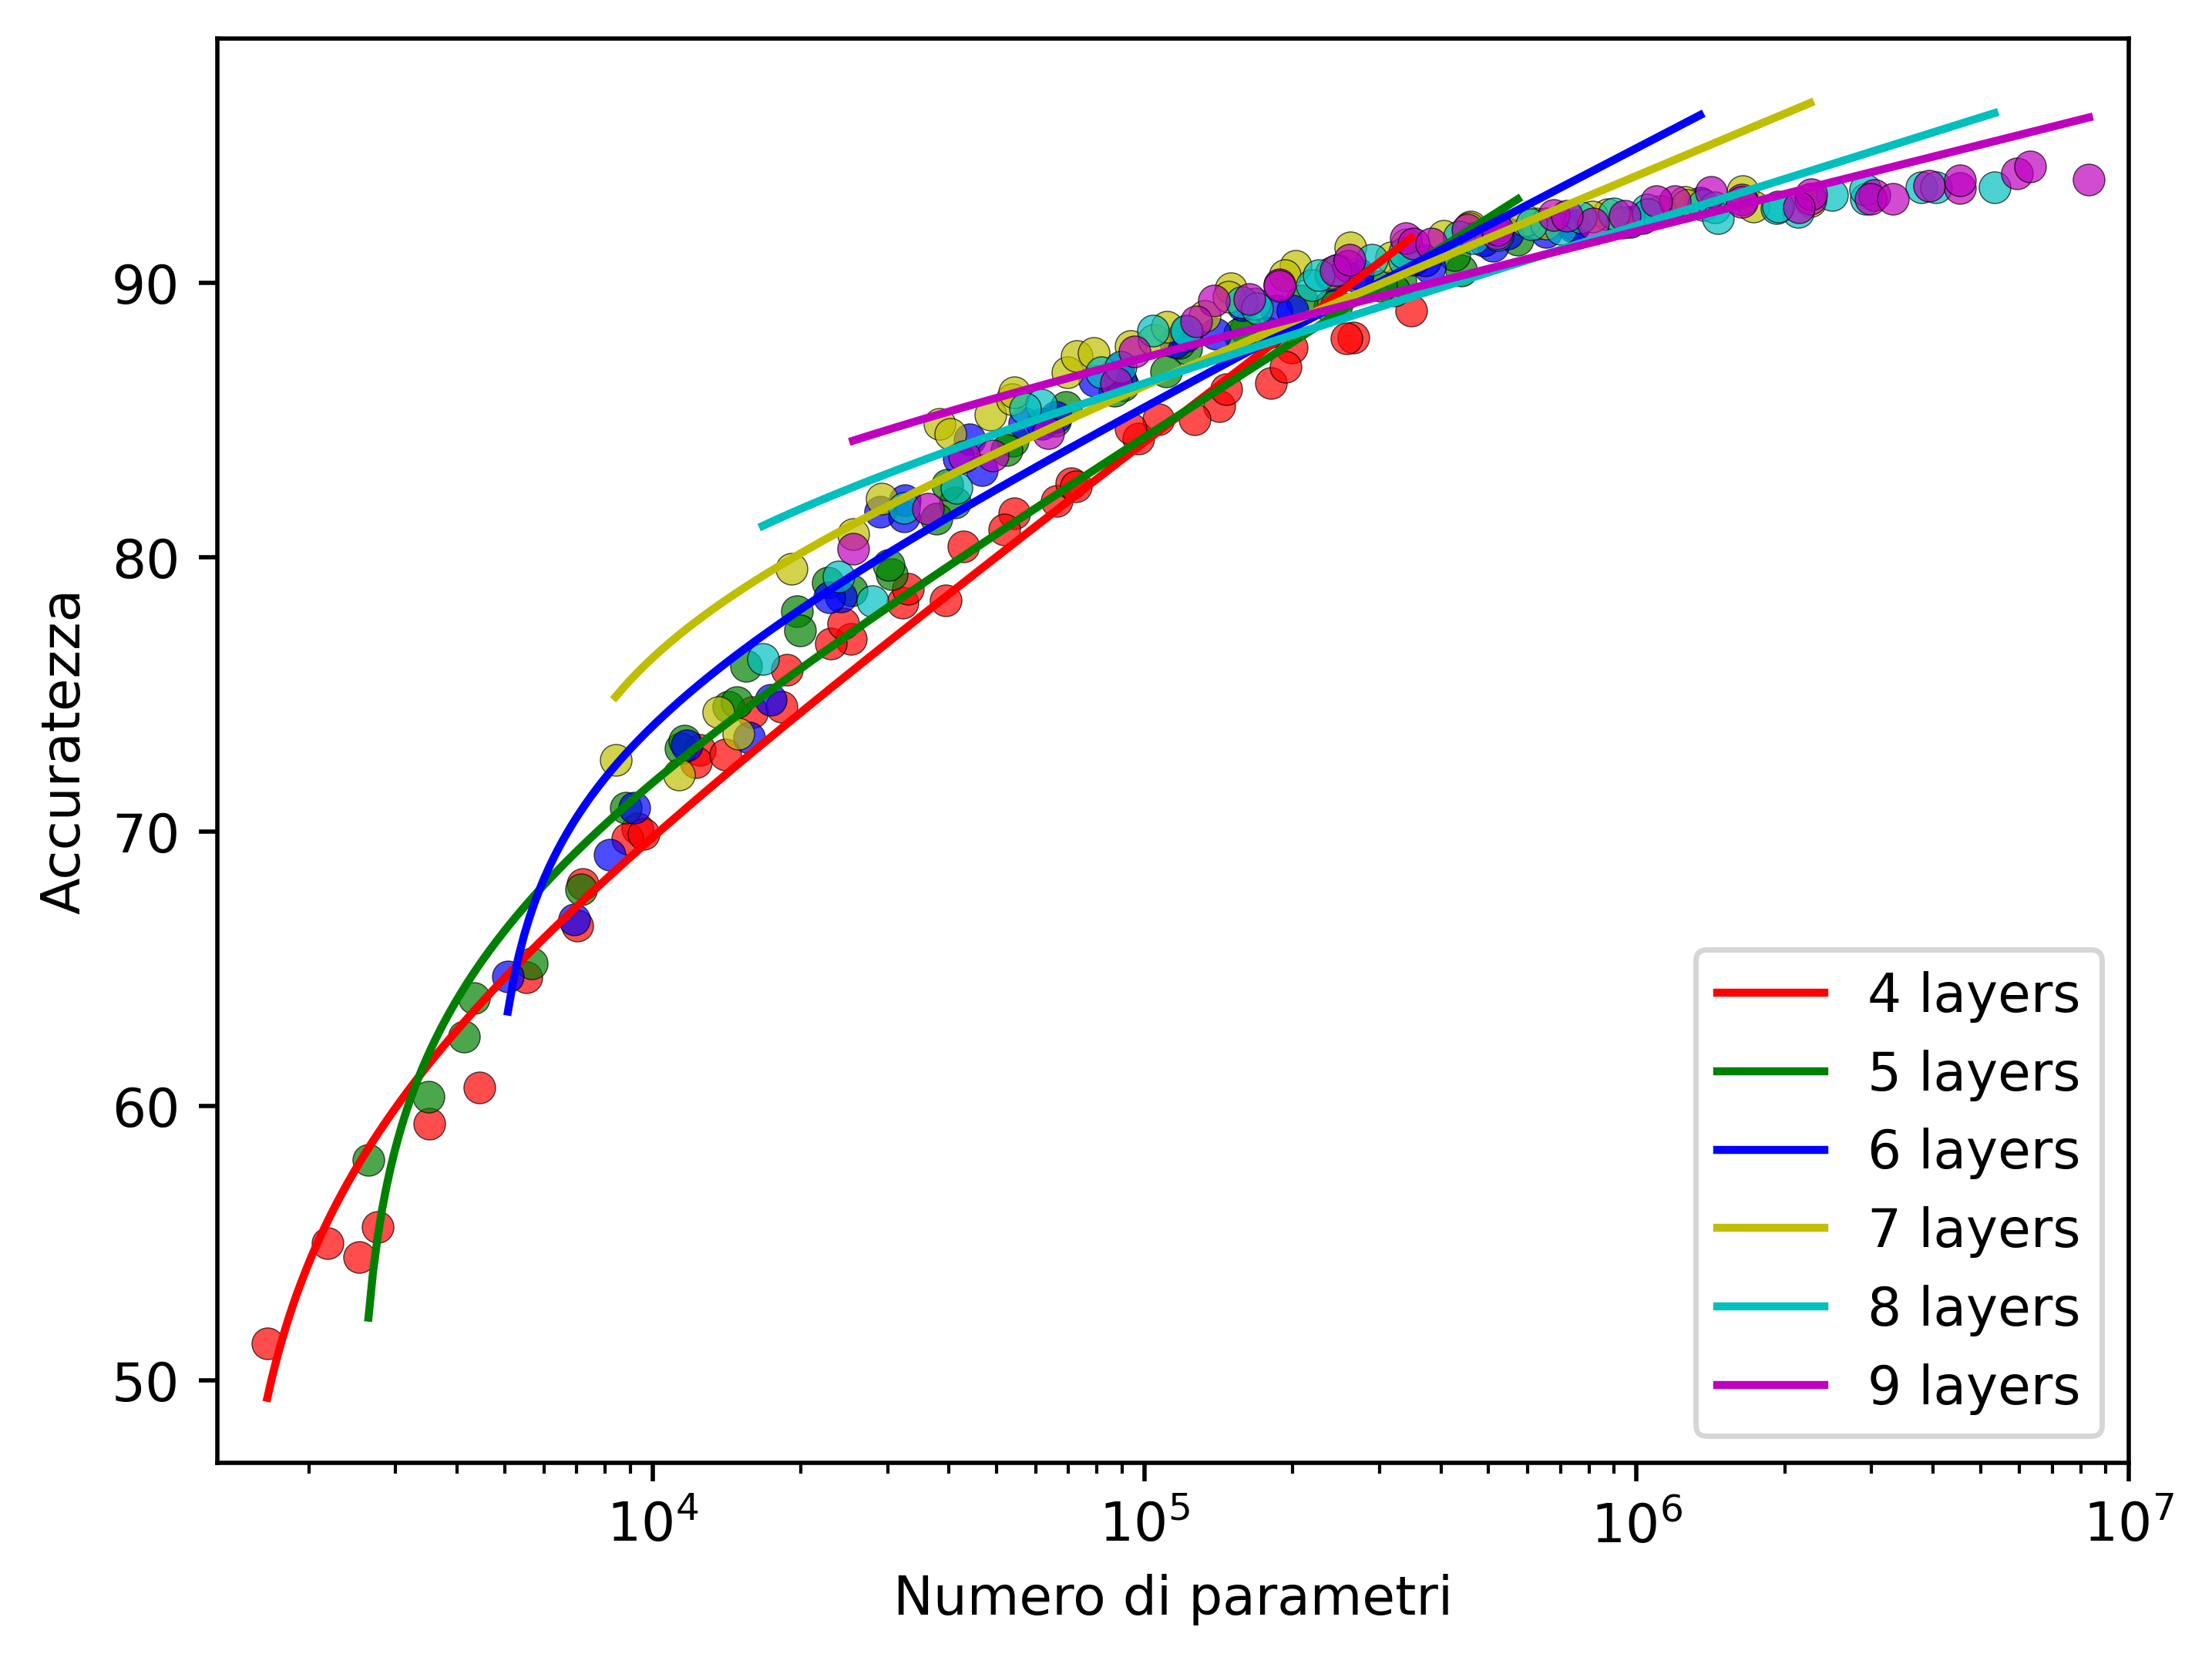
\includegraphics[width=0.4\textwidth]{tesi/immagini/log_reg_log.png}}\quad
    \caption{\textit{Regressione logaritmica}.}
    \label{fig:log_reg}
\end{figure}

Anche un modello di questa tipologia (\ref{fig:log_reg}) non sembra l'ideale per approssimare al meglio la distribuzione di dati a disposizione. Sebbene l'introduzione di un asintoto verticale aiuti ad adattare il modello per valori bassi di parametri, rimane un grande problema di generalizzazione per valori elevati di occupazione di memoria. Questo è dovuto al fatto che la funzione logaritmica è di natura monotona crescente e di conseguenza non converge ad un valore sulle ordinate come accade con modelli che dispongono di un asintoto orizzontale; ciò ha l'effetto di sovrastimare le prestazioni di una rete con un numero elevato di parametri.

\subsubsection{Combinazione convessa tra funzione logaritmica ed esponenziale}

Entrambe le regressioni, esponenziale e logaritmica, tendono ad approssimare bene l'andamento dei dati nella parte iniziale delle curve mentre faticano ad adattarsi adeguatamente ai risultati per elevati valori di numero di parametri, e quindi a generalizzare i risultati in un range diverso da quello osservato. In particolare le funzioni esponenziali tendono a sottostimare l'accuratezza per una rete con un elevato numero di parametri, invece le funzioni logaritmiche tendono a sovrastimarla. 
Diventa quindi legittimo supporre che l'effetto combinato di questi due tipi di modelli possa migliorare la precisione di predizione della funzione risolvendo i problemi di generalizzazione per un elevato numero di parametri.

Una funzione matematica che combina l'andamento di diverse tipologie di curve può essere ottenuta tramite la scelta di determinati moltiplicatori che vanno a determinare quanto una certa funzione incide sul calcolo del risultato. Per rendere la scelta di questi moltiplicatori il più imparziale e precisa possibile è possibile parametrizzarli sotto forma di un'unica variabile $k$ che modella la funzione matematica secondo la formula \ref{eq:comb1}.

\begin{equation}
\label{eq:comb1}
    \centering
    acc = k \cdot (-a^{P - b} + c) + (1 - k) \cdot (d \cdot log(P - e) + f)
\end{equation}

L'equazione \ref{eq:comb1} può essere riscritta in maniera semplificata come in \ref{eq:comb2}, riducendone i gradi di libertà per rendere più facile trovare i parametri del modello. Infatti entrambi i parametri $c$ ed $f$ regolano la traslazione lungo l'asse verticale della curva e possono essere riscritti sotto forma di un'unica variabile $c$.

\begin{equation}
\label{eq:comb2}
    \centering
    acc = -k \cdot a^{P - b} + (1 - k) \cdot (d \cdot log(P - e)) + c
\end{equation}

In questa situazione i parametri $a$, $b$, $c$, $d$, $e$ si comportano analogamente a quanto spiegato in precedenza, mentre il parametro $k$ può assumere valori interni all'intervallo [0, 1] e regola la dominanza della funzione logaritmica e di quella esponenziale sul modello finale. Nello specifico per $k=0$ si ottiene lo stesso andamento della funzione logaritmica, per $k=1$ si ha invece la funzione esponenziale e per $k=0.5$ si otterrebbe la media aritmetica delle due curve.

\begin{figure}[ht]
    \centering
    \subfloat[]{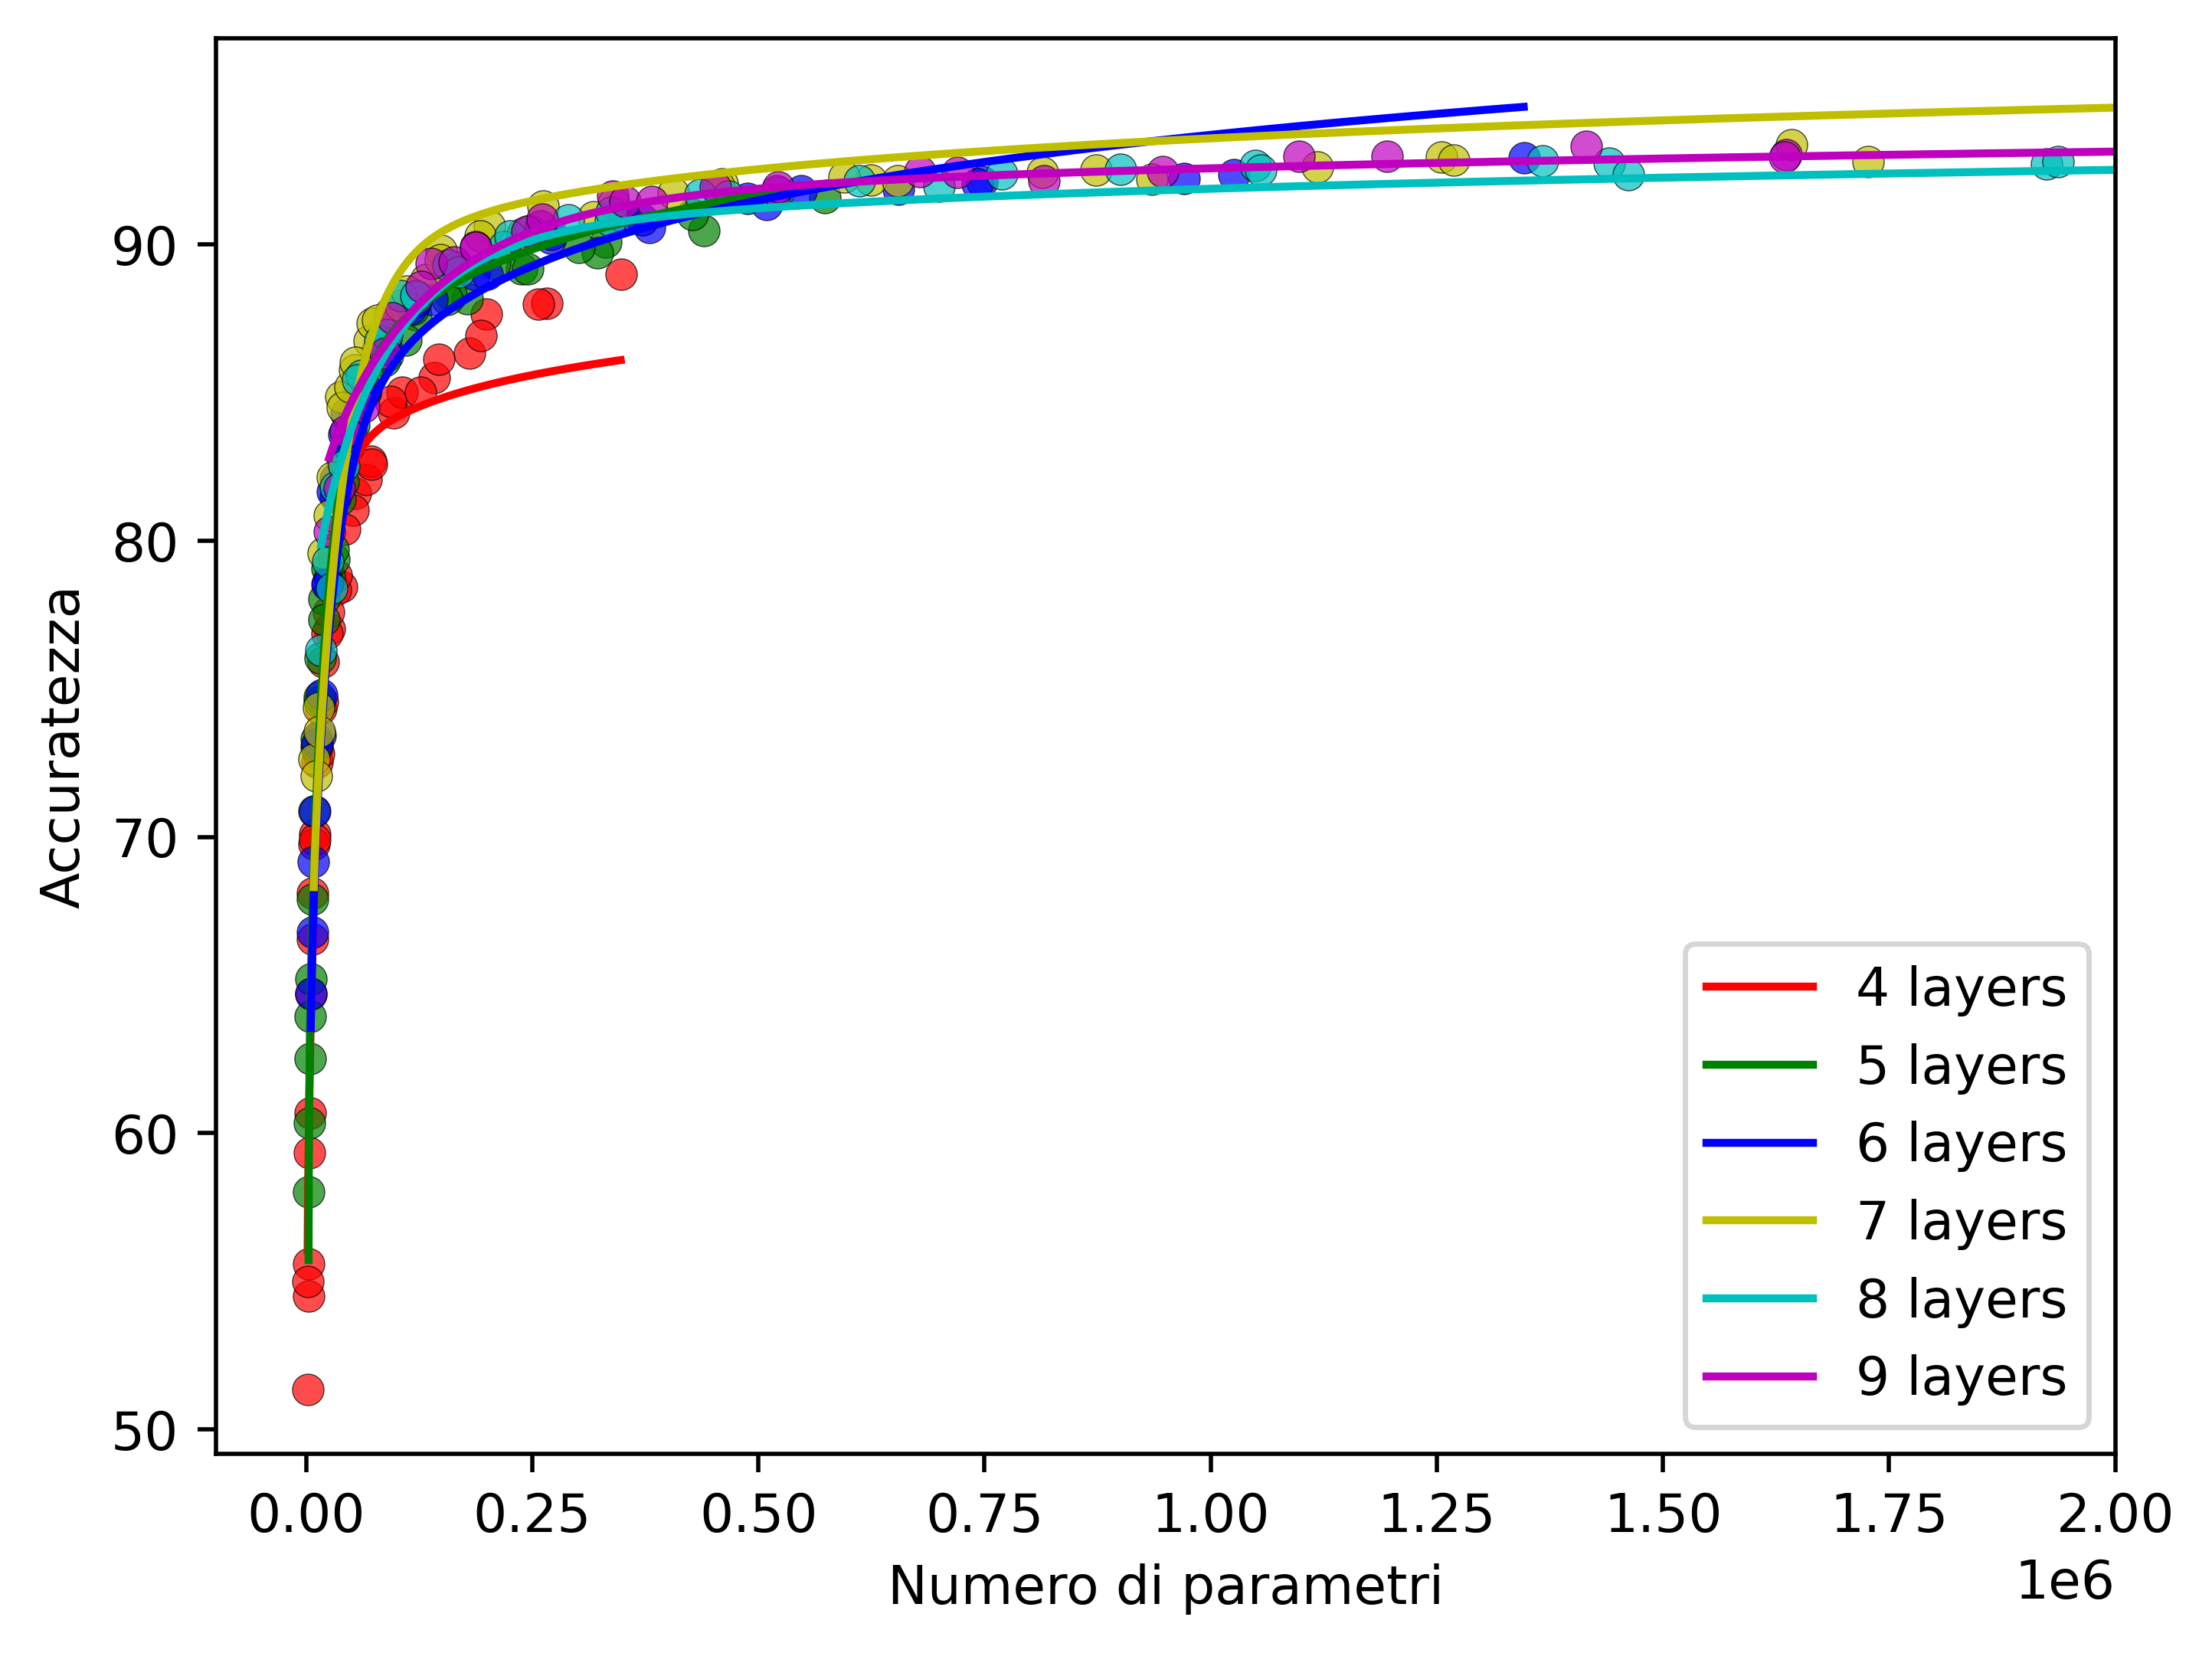
\includegraphics[width=0.4\textwidth]{tesi/immagini/comb_reg.png}}\quad
    \subfloat[]{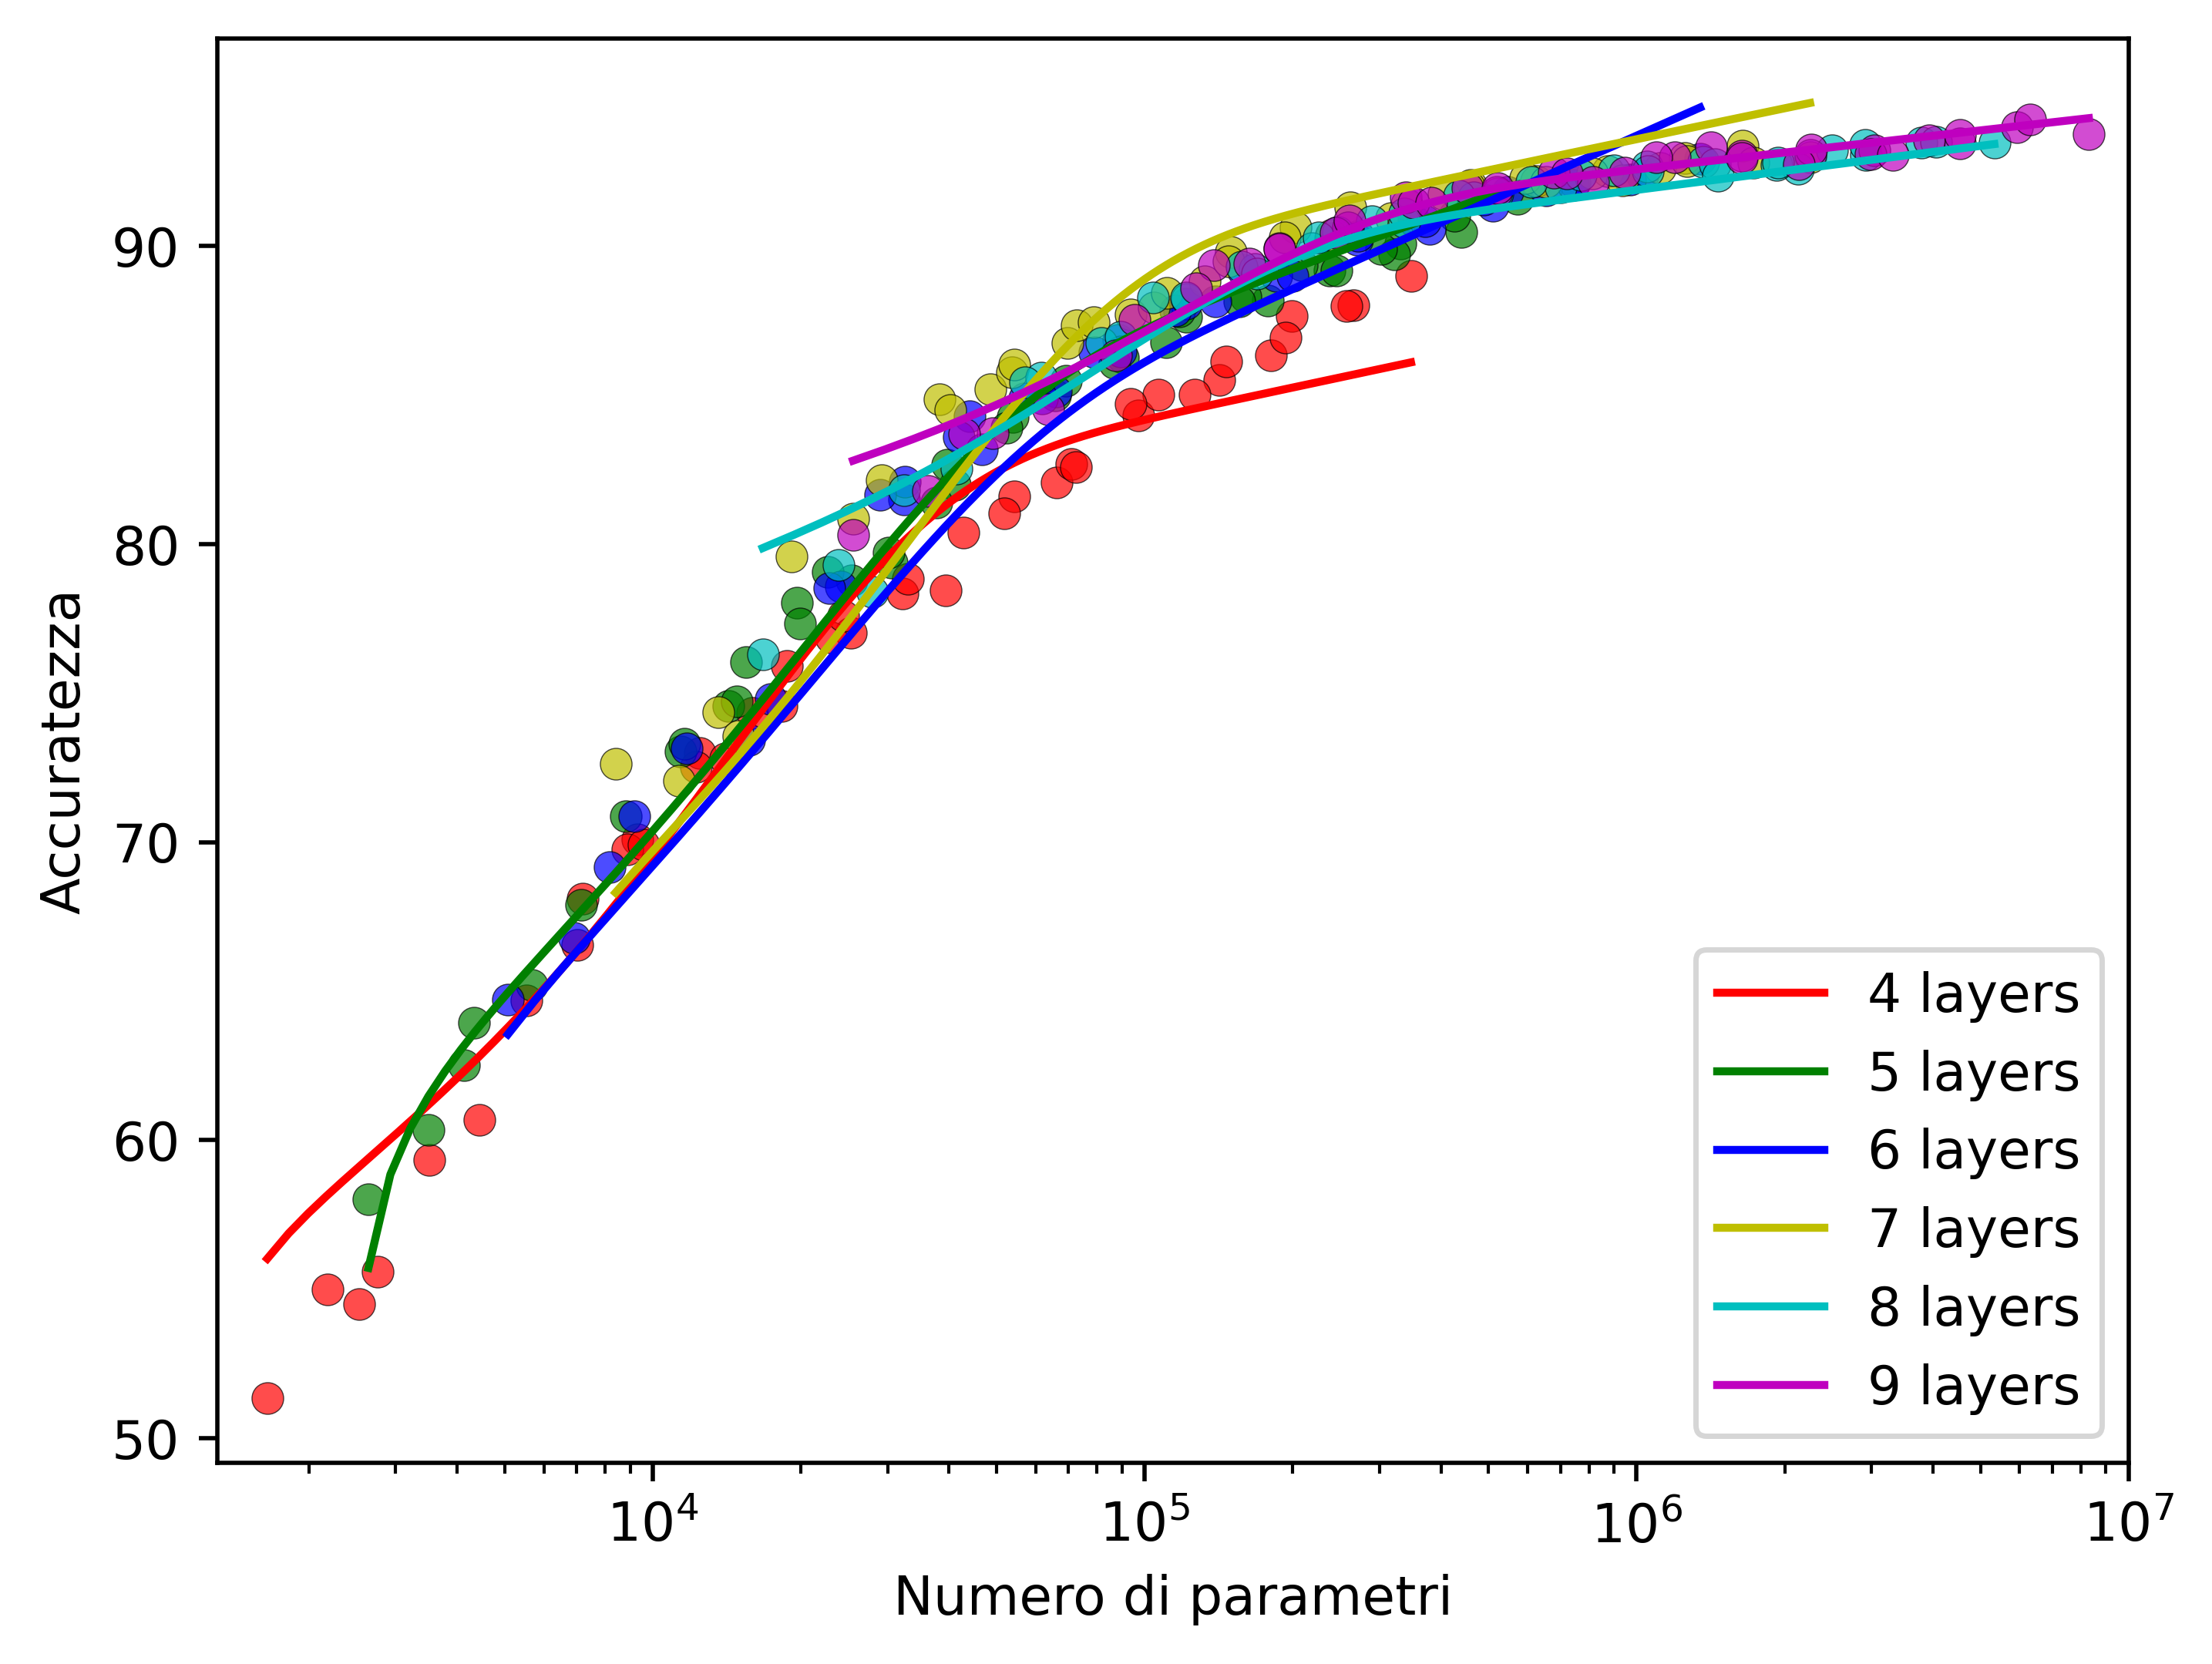
\includegraphics[width=0.4\textwidth]{tesi/immagini/comb_reg_log.png}}\quad
    \caption{\textit{Regressione logaritmica}.}
    \label{fig:comb_reg}
\end{figure}

Sebbene questo modello mostri miglioramenti sull'adattamento generale della curva alla distribuzione di dati, è evidente come per elevati valori di numero di parametri la funzione segua l'andamento logaritmico e continui quindi a crescere monotonicamente; ciò è chiaro osservando la figura \ref{fig:comb_reg} (b) in quanto la regressione si adagia sull'asintoto obliquo presente per l'influenza logaritmica della funzione.

\subsubsection{Regressione iperbolica}

È evidente che le regressioni proposte in precedenza non sono adatte per poter studiare determinati intervalli di parametri in cui sia più opportuno scegliere un certo valore di numero di layer ($N$); il principale problema dei modelli proposti sono la scarsa capacità di estrapolazione delle curve a valori nuovi di numero di parametri. % distribuzione di dati ed il fatto che non si riesca ad approssimarne l'andamento per alti valori di numero di parametri e quindi a generalizzare. 

Una funzione che potrebbe ovviare a questi problemi è quella iperobolica, osservando infatti un ramo d'iperbole di questa tipologia $y= -\frac{1}{x}$, nel semipiano delle ascisse positive, si può notare una certa somiglianza con le distribuzioni in figura \ref{fig:dati_layer} (a). La famiglia delle funzioni iperboliche è caratterizzata da due diversi asintoti, uno verticale, utile per delimitare in questo caso il grafico verso sinistra, ed uno orizzontale, necessario per porre un limite di accuratezza massimo verso cui convergere ed evitare i problemi visti con le funzioni iperboliche che crescono monotonicamente. 

Il vantaggio delle funzioni iperboliche rispetto a quelle esponenziali per quanto riguarda l'asintoto orizzontale risiede nel fatto che, pur convergendo entrambe al valore imposto dalla retta orizzontale, l'iperbole lo fa più lentamente, mentre l'esponenziale ci arriva in maniera immediata, senza fornire informazioni molto utili sulla differenza qualitativa tra punti distanti fra loro.

La relazione tra accuratezza di classificazione e numero di parametri può quindi essere modellata tramite l'equazione \ref{eq:hyp}.

\begin{equation}
\label{eq:hyp}
    \centering
    acc = -\frac{a}{P - b} + c
\end{equation}

In una funzione iperbolica di questa tipologia si suppone che tutti e tre i parametri $a$, $b$, $c$ assumano valori positivi, in modo da mantenere coerente l'andamento della curva senza ribaltamenti indesiderati. In particolare $a$ regola la pendenza della funzione, mentre $b$ e $c$ sono responsabili della posizione rispettivamente dell'asintoto verticale e di quello obliquo della curva, ovvero della sua traslazione lungo gli assi cartesiani.

\begin{figure}[ht]
    \centering
    \subfloat[]{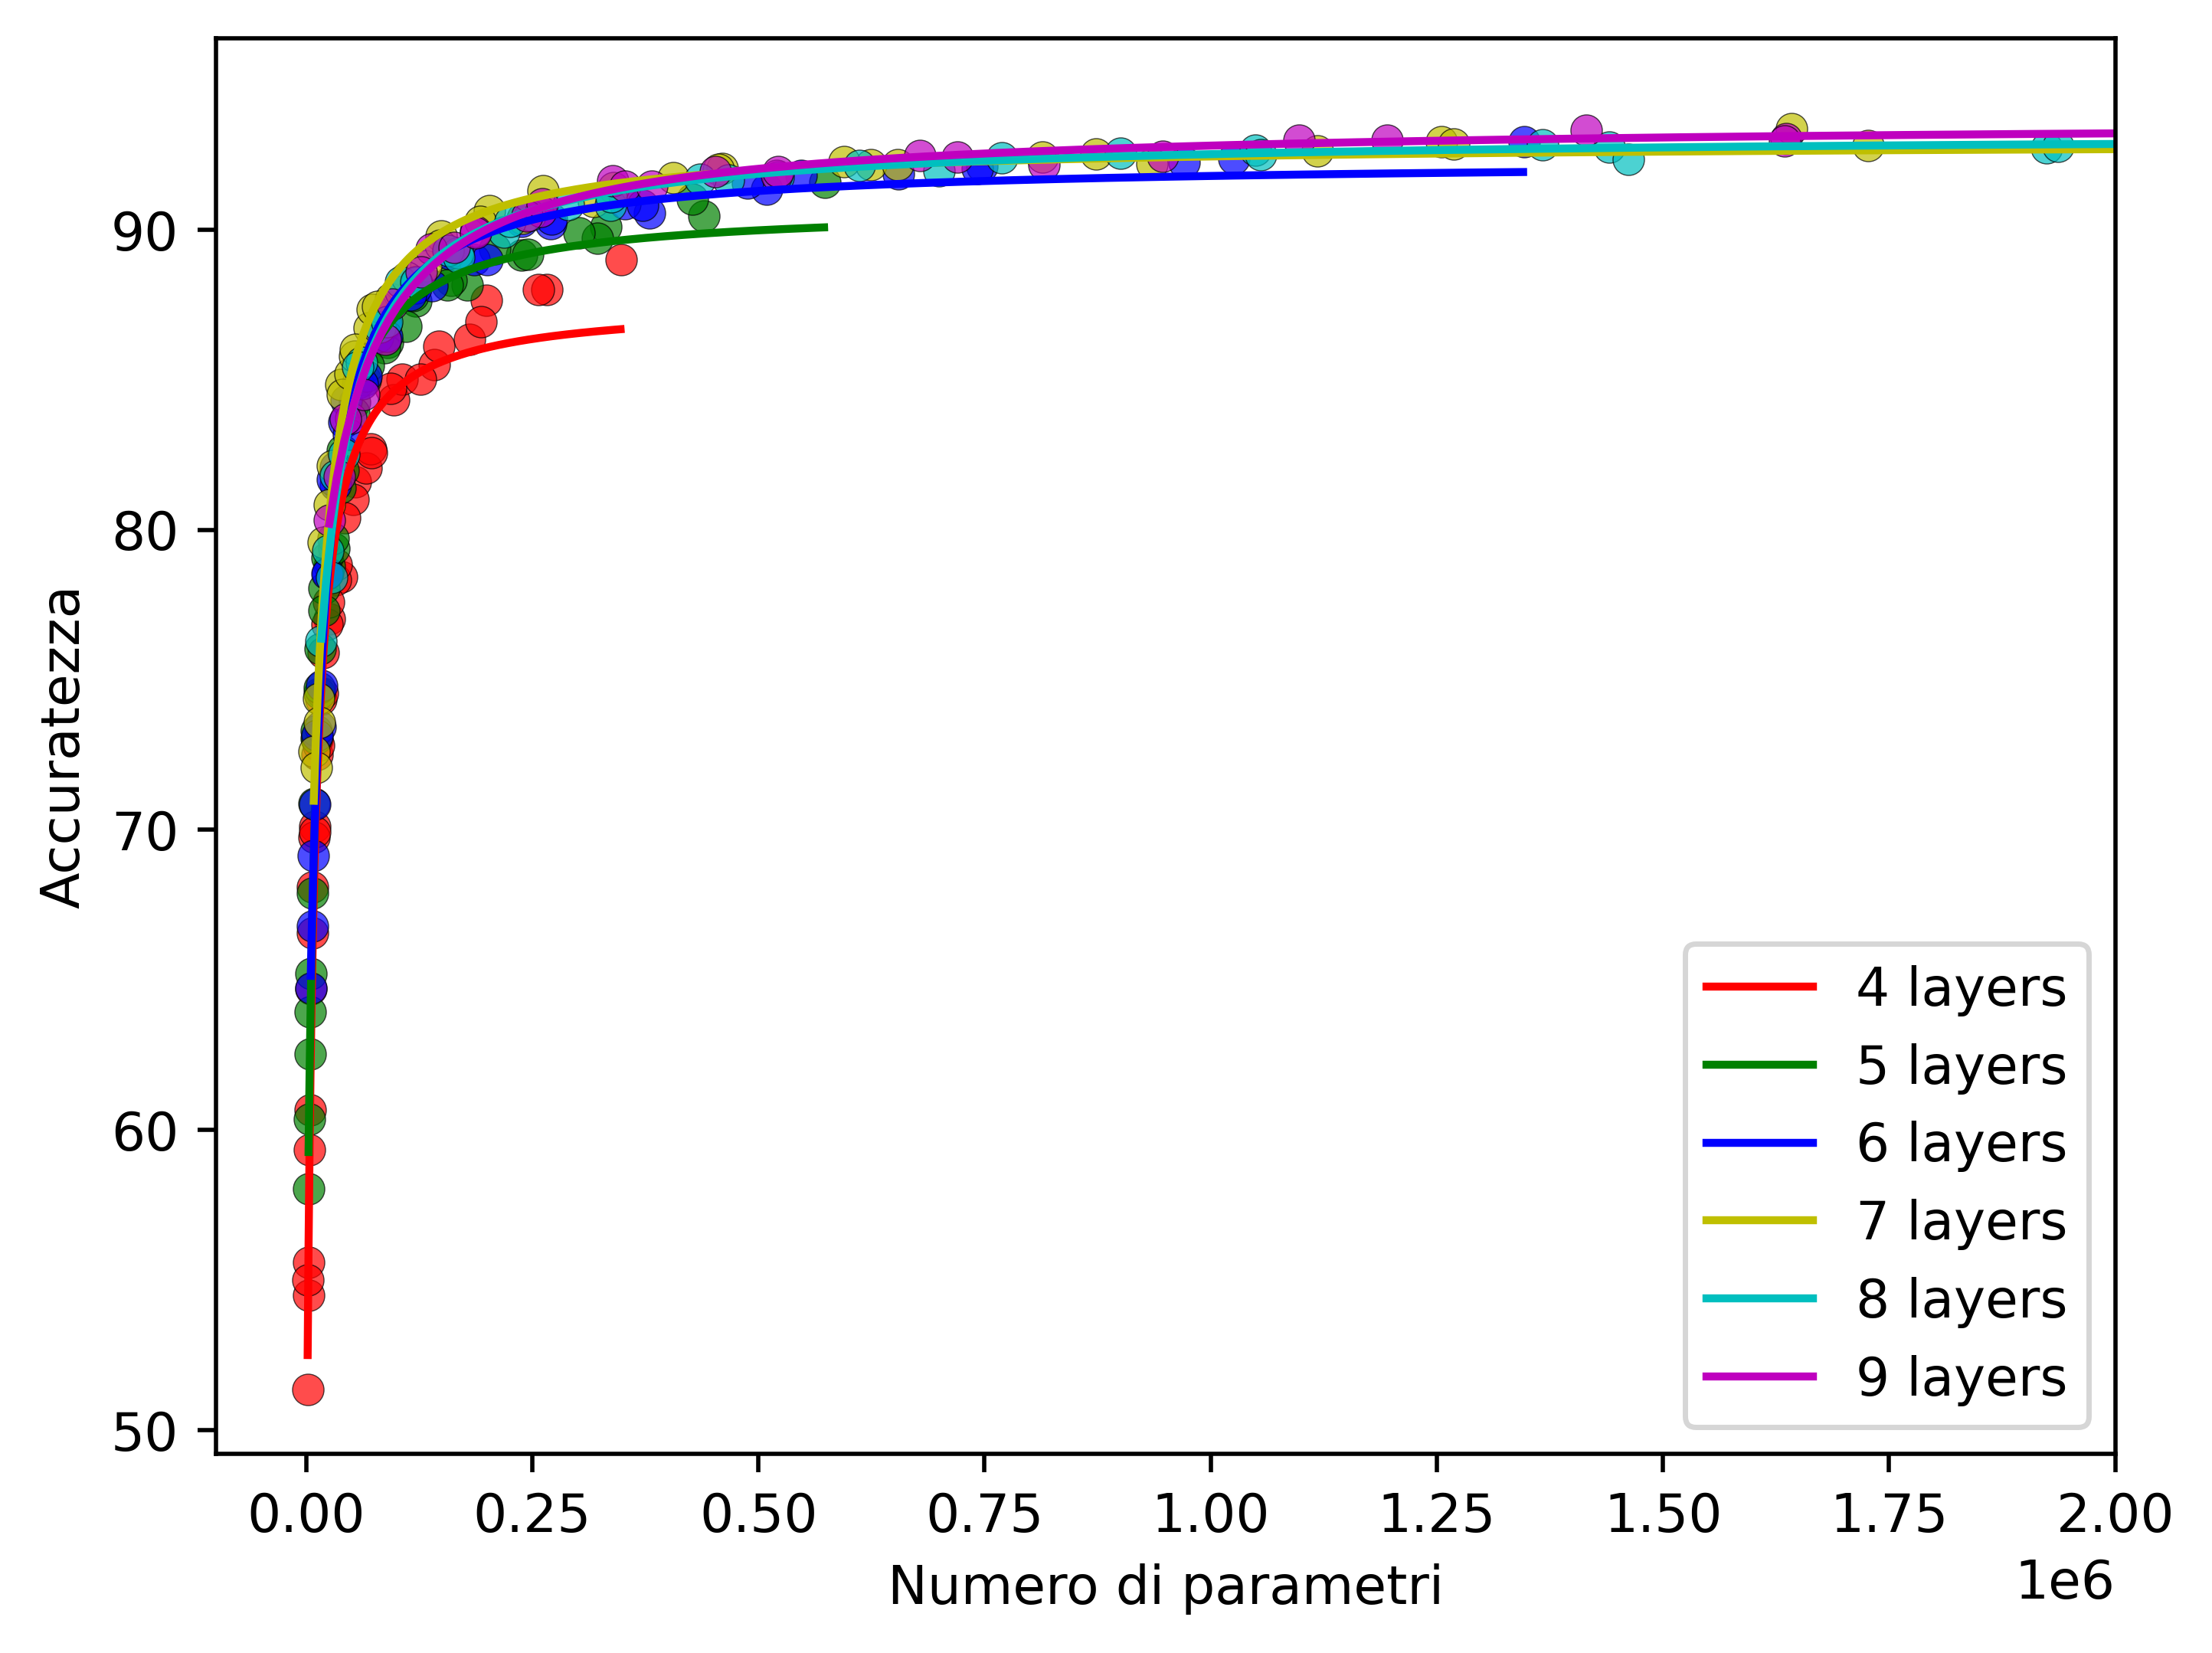
\includegraphics[width=0.4\textwidth]{tesi/immagini/hyp_reg.png}}\quad
    \subfloat[]{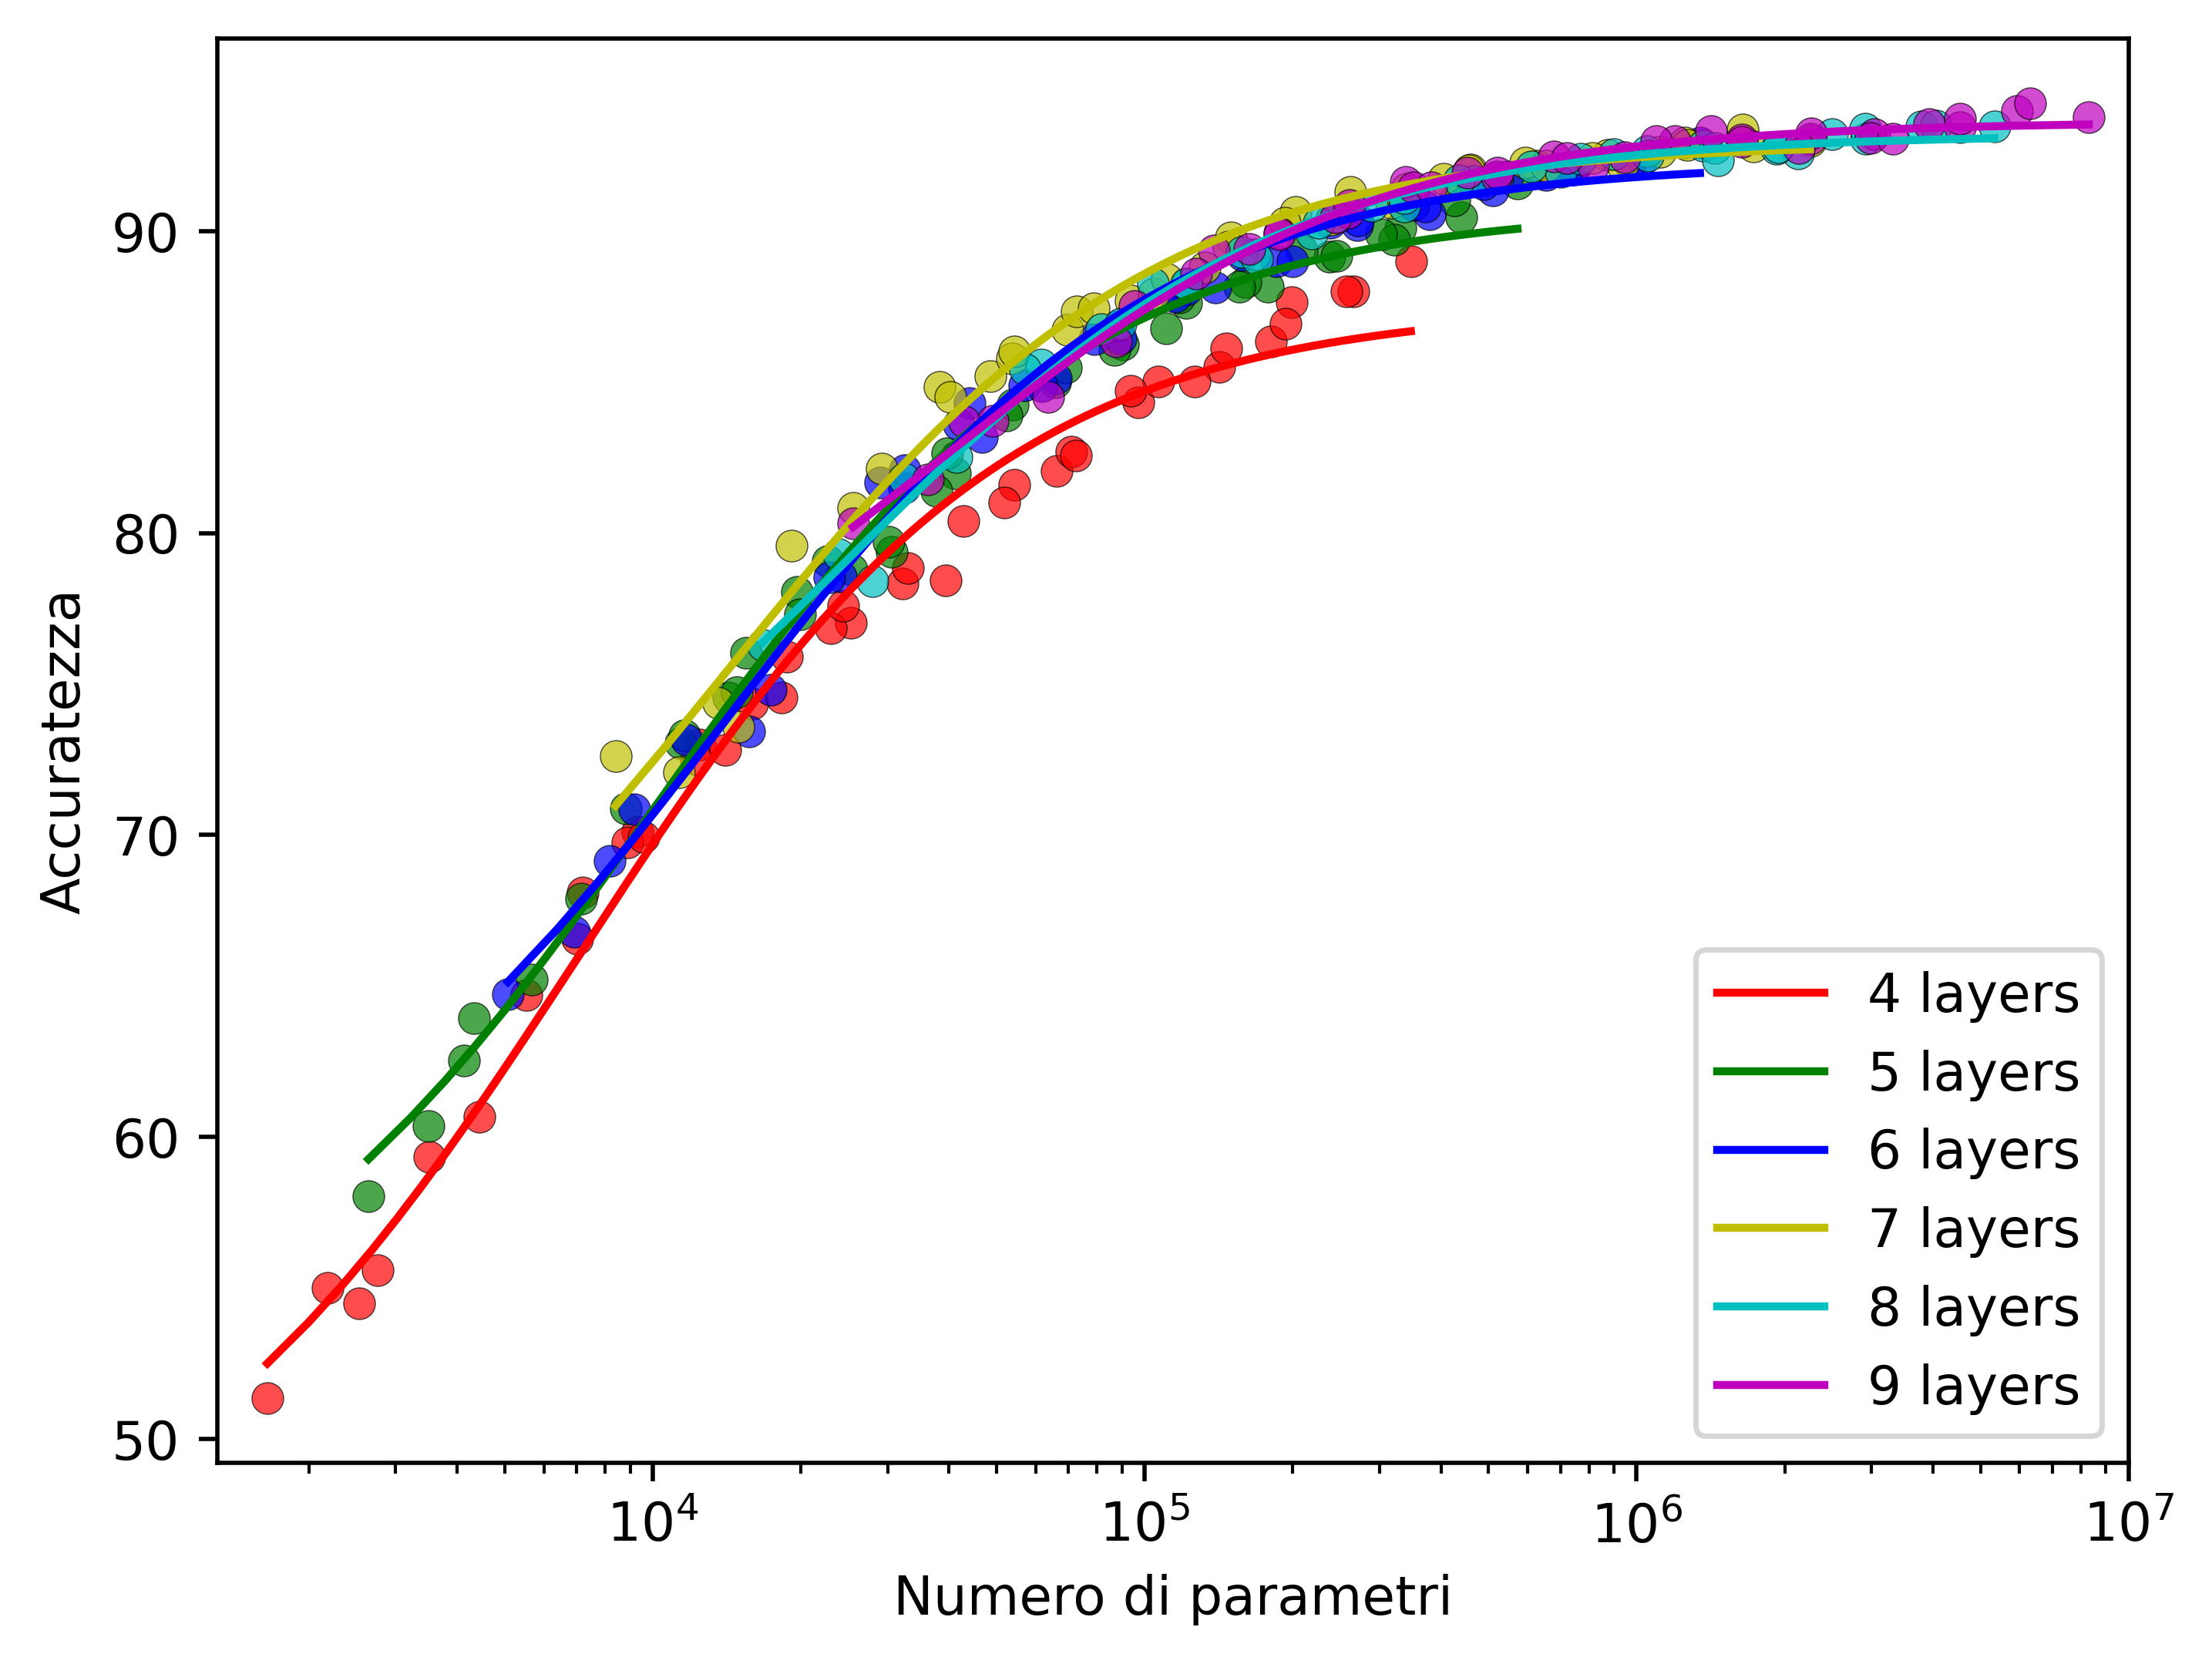
\includegraphics[width=0.4\textwidth]{tesi/immagini/hyp_reg_log.png}}\quad
    \caption{\textit{Regressione iperbolica}.}
    \label{fig:hyp_reg}
\end{figure}

Nonostante i miglioramenti su scala lineare possano sembrare lievi, si riesce ad apprezzare su scala logaritmica l'incremento di precisione di predizione e di adattamento generale ai dati a disposizione. 

La scelta della famiglia delle funzioni iperboliche sembra quindi essere vincente, rimane tuttavia da risolvere il problema di adattamento delle curve per alti valori di numero di parametri, si nota per esempio la discrepanza tra i risultati di predizione ed i dati reali corrispondenti a circa centodiecimila parametri per quanto riguarda le PhiNets con 4 layers (colore rosso in figura \ref{fig:hyp_reg}).


\subsubsection{Regressione iperbolica generalizzata}

Un modo per migliorare ulteriormente il modello di regressione iperbolico è quello di considerare un ulteriore grado di libertà che in precedenza è stato impostato implicitamente ad un valore fisso. Le funzioni iperboliche considerate fino ad ora, infatti, possono essere lette in maniera semplificata come una frazione del tipo $y= -\frac{1}{x^{1}}$, in cui l'esponente della variabile indipendente è fissato al valore unitario. 

Si possono quindi ampliare i gradi di libertà della funzione per contenere anche un fattore di potenza all'esponente della variabile indipendente. In particolare la nuova funzione di regressione iperbolica ottimizzata segue la relazione descritta dall'equazione \ref{eq:hyp+}.

\begin{equation}
\label{eq:hyp+}
    \centering
    acc = -\frac{a}{P^{\phi}} + c
\end{equation}

In questa funzione i parametri $a$ e $c$ si comportano esattamente come descritto per la funzione iperbolica, mentre il fattore di potenza $\phi$, che può assumere solamente valori positivi (per mantenere l'andamento iperbolico desiderato), regola la forma della curva. 

È inoltre importante notare come nel modello descritto dalla formula \ref{eq:hyp+} sia venuto a meno il parametro $b$ presente precedentemente, questa scelta segue il principio del rasoio di Occam dato che il parametro assumeva valori irrilevanti per le grandezze considerate.

\begin{figure}[ht]
    \centering
    \subfloat[]{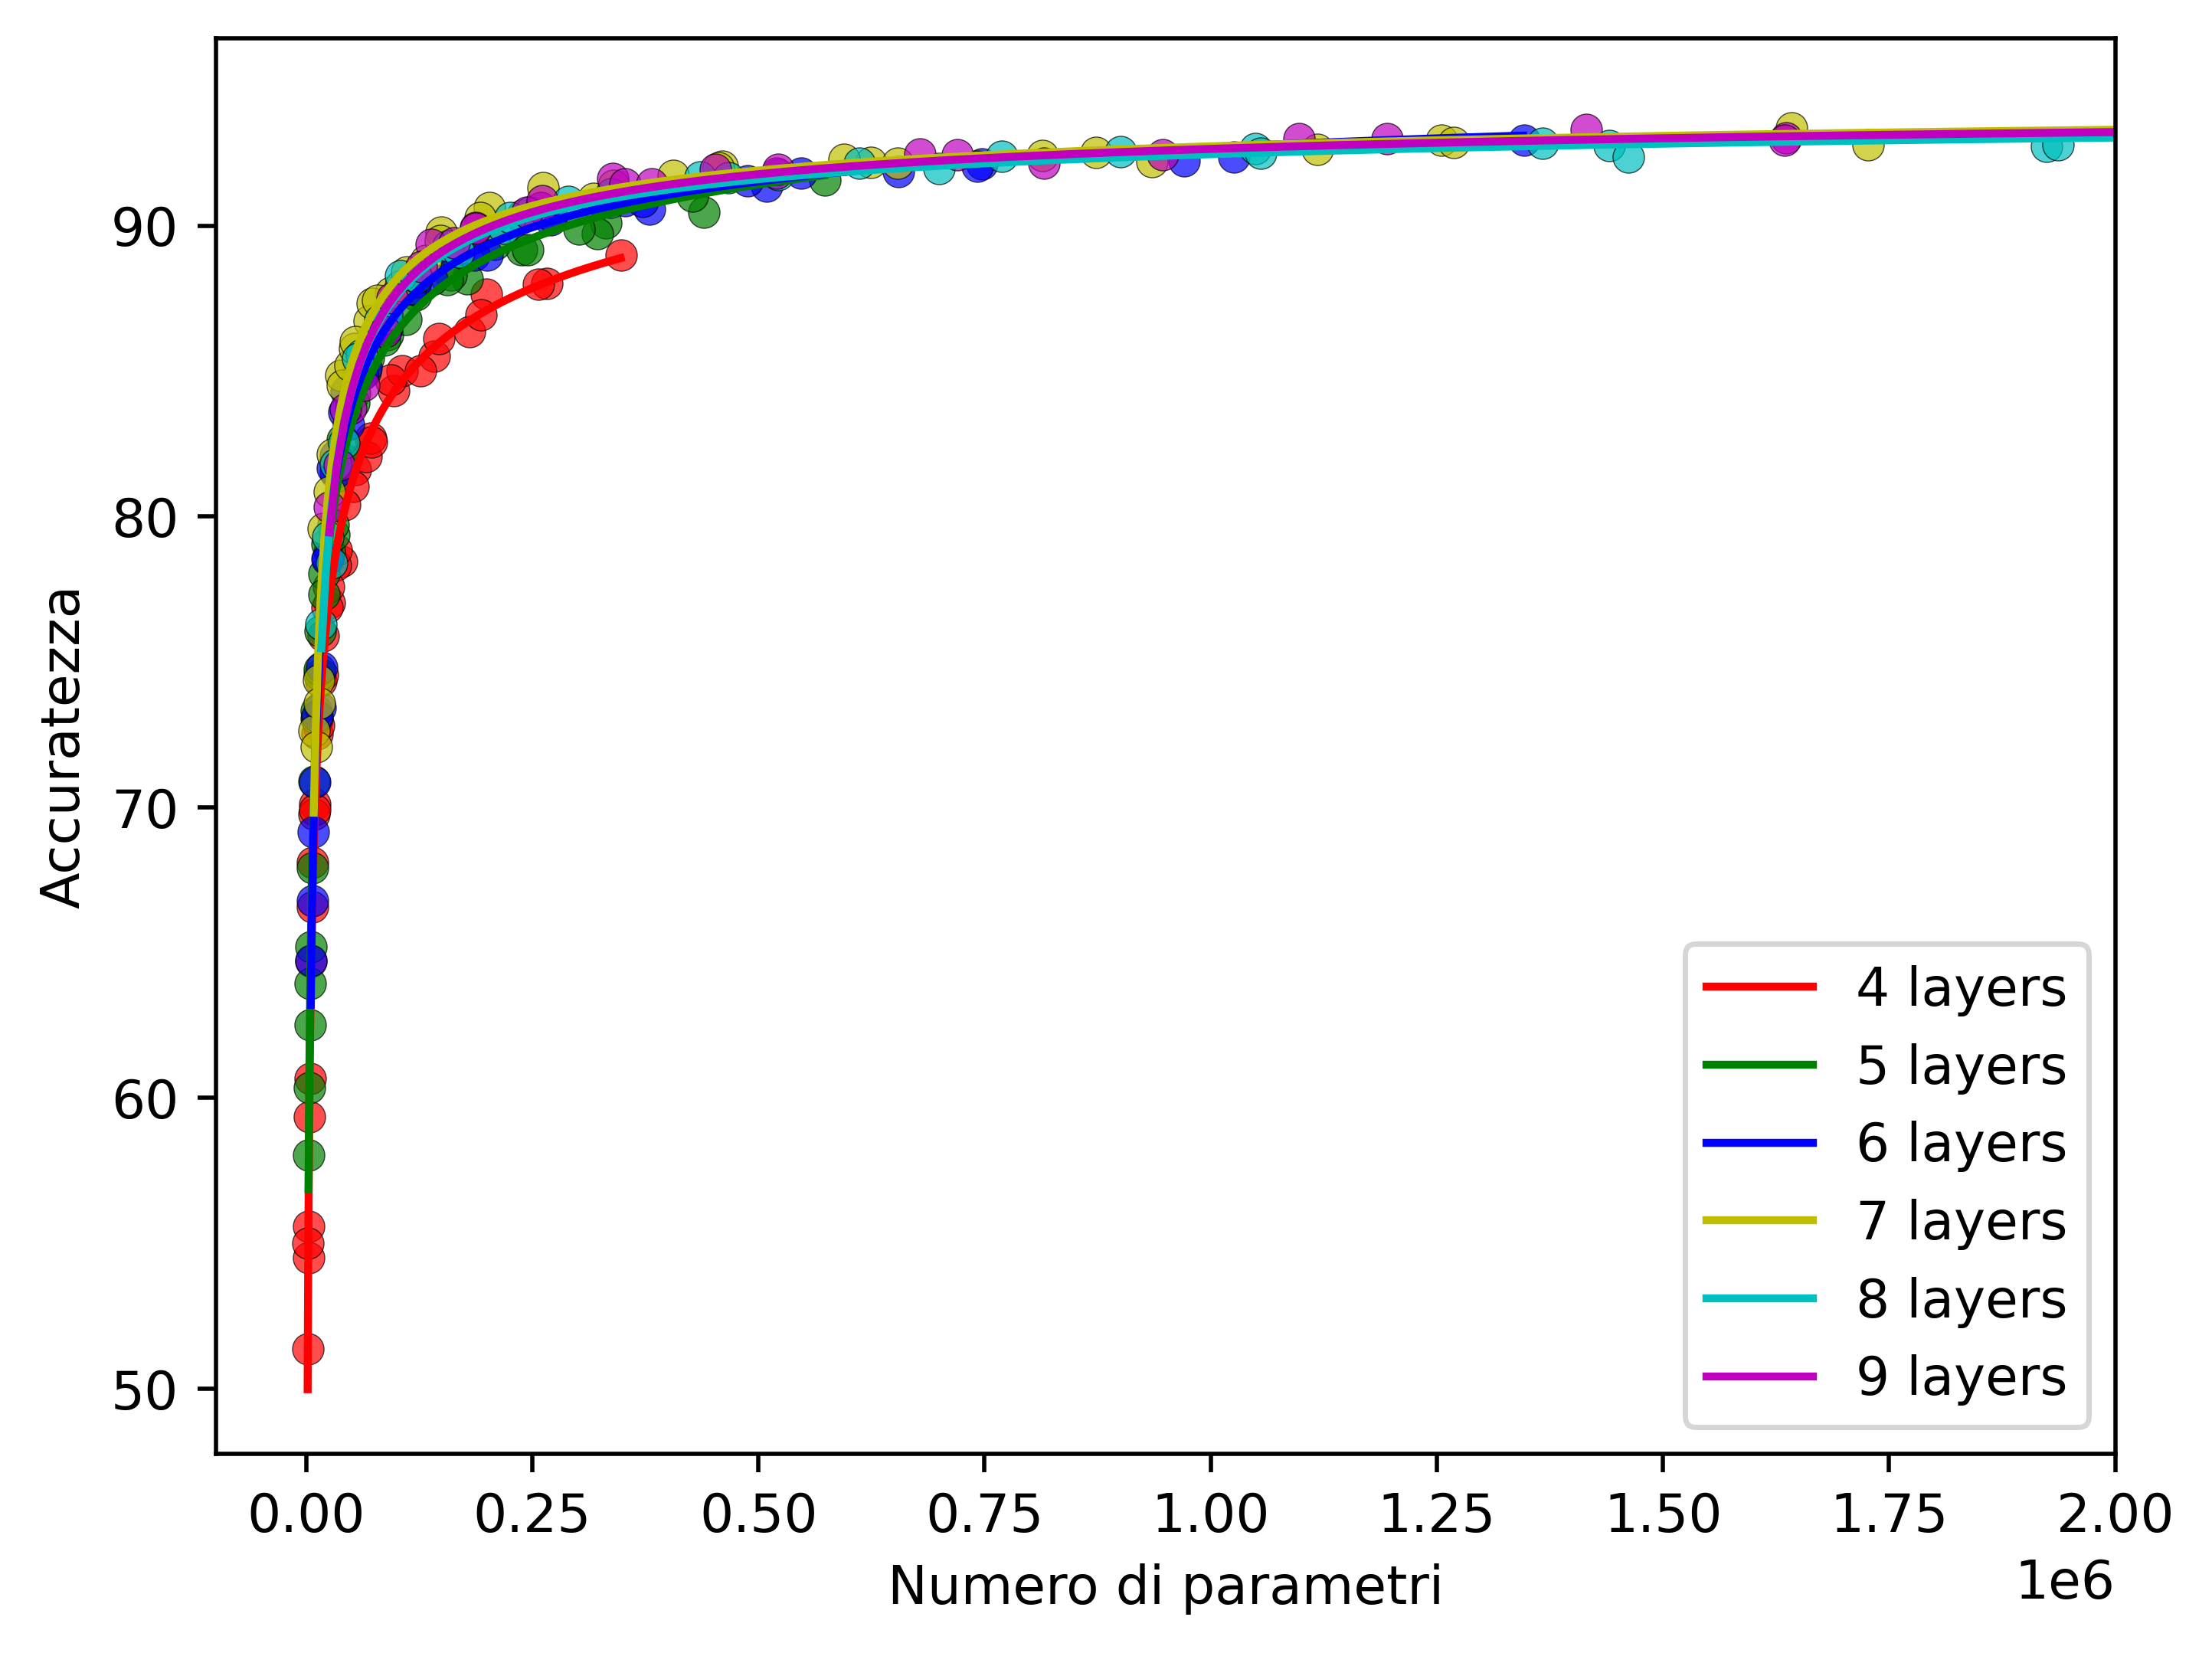
\includegraphics[width=0.4\textwidth]{tesi/immagini/hyp+_reg.png}}\quad
    \subfloat[]{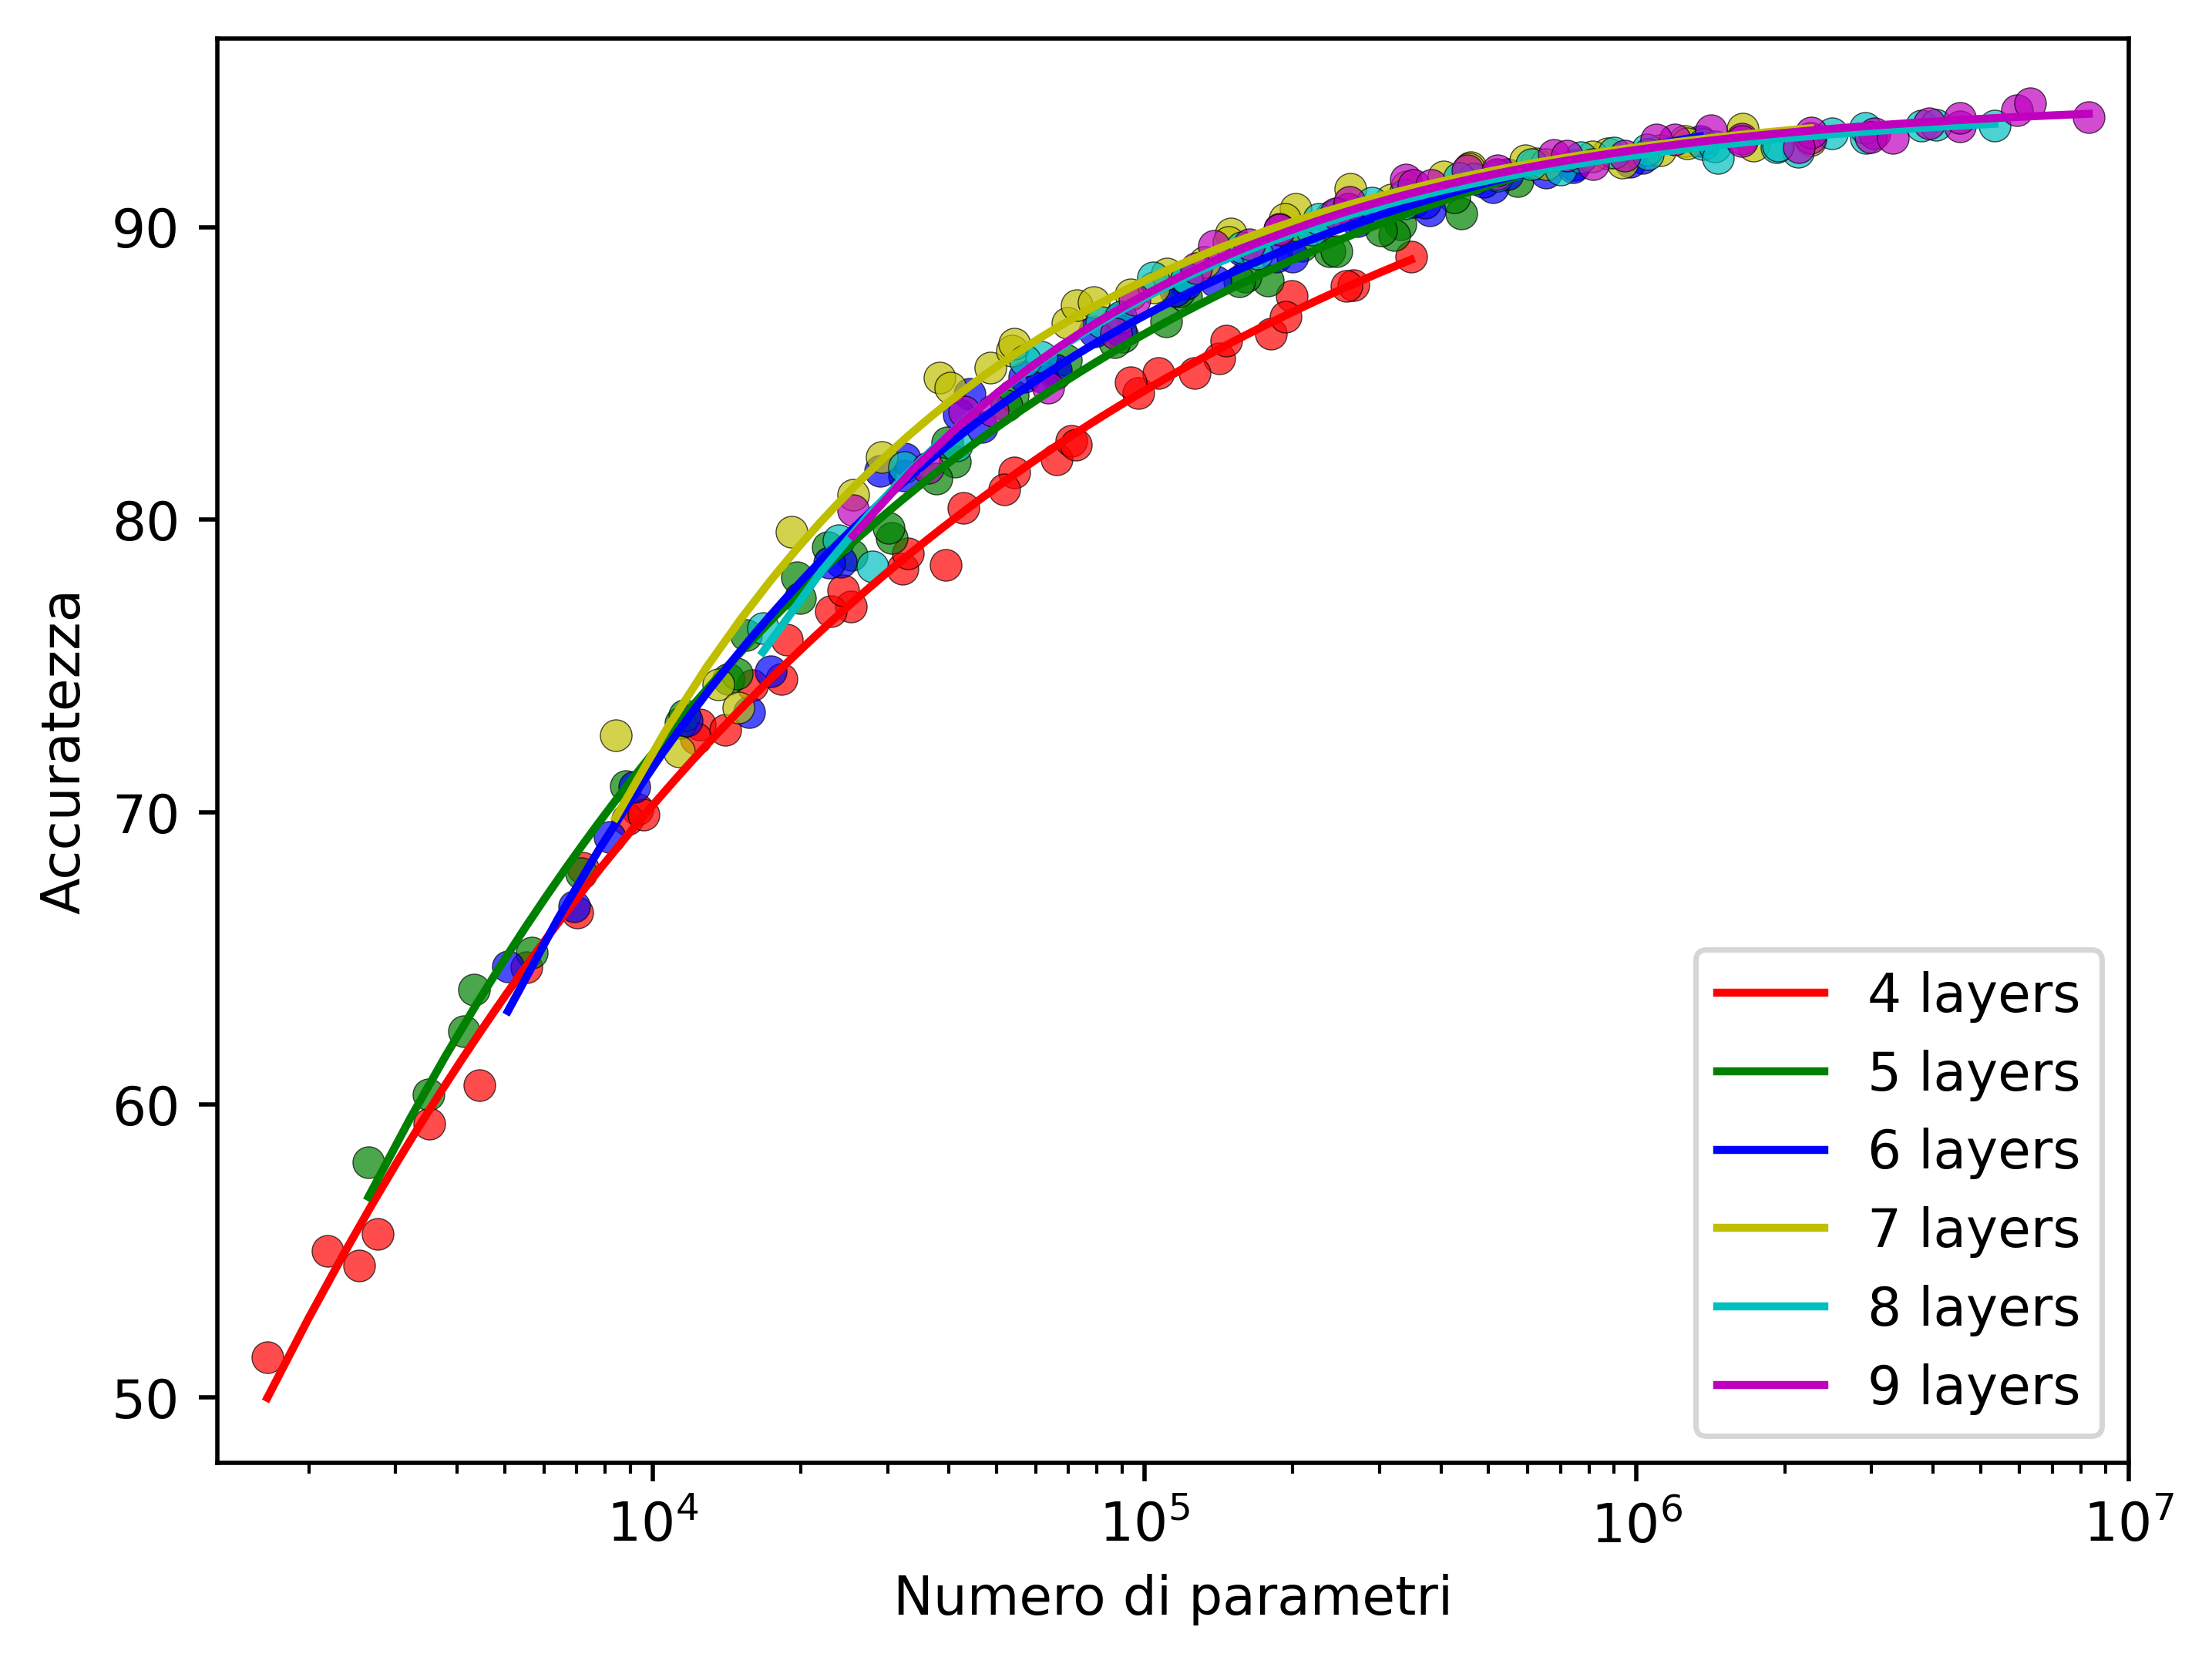
\includegraphics[width=0.4\textwidth]{tesi/immagini/hyp+_reg_log.png}}\quad
    \caption{\textit{Regressione iperbolica ottimizzata}.}
    \label{fig:hyp+_reg}
\end{figure}

Questo modello di regressione sembra essere il migliore per tutti i criteri presi in considerazione, l'adattamento generale delle curve alla distribuzione dei dati è ottimale, gli estremi sinistri e destri sono ben approssimati e sono presenti sia un asintoto verticale, corrispondente all'asse $parametri=0$, sia uno orizzontale, che varia in base al numero di layer considerato. Inoltre, come ci si potrebbe aspettare, all'aumentare del numero di layer cresce anche l'ordinata dell'asintoto orizzontale di accuratezza e ciò è un risultato ragionevole dato che ci si aspetta una correlazione positiva tra il numero di parametri di una rete (che cresce linearmente con il numero di layer) e la sua accuratezza di classificazione.

\subsection{Metodi di segmentazione}

Essendo l'obiettivo della ricerca quello di determinare il miglior valore di $N$ (numero di strati convoltivi) che ottimizza le prestazioni di una PhiNet per un determinato budget di numero di parametri, sono d'aiuto alcune tecniche di segmentazione di dati che permettono di determinate gli intervalli sull'asse dei parametri all'interno dei quali sia più vantaggioso scegliere un preciso valore di $N$ per inizializzare la rete più performante.

Sia partendo dalla distribuzione dati originaria, sia dalle funzioni di regressione è possibile, con le giuste tecniche, ottenere una divisione tra intervalli in cui sia esplicito quale valore di numero di layer sia il migliore per ogni range.

Osservando solamente i dati originariamente raccolti dal punto di vista del numero di strati convolutivi  è già possibile fornire una stima empirica su quale valore di $N$ sia il migliore per un certo budget di numero di parametri. Dalla figura \ref{fig:dati_layer} si può ad esempio notare come per un valore di circa duecentomila parametri a disposizione la scelta peggiore per il numero di layer sia 4 (colore rosso), mentre sia molto vantaggioso scegliere una configurazione di rete con 7 strati convolutivi (colore giallo). Questo semplice processo di confronto andrebbe ripetuto molteplici volte in modo da ottenere dati sufficienti per stimare dei possibili intervalli in cui la scelta migliore di $N$ sia comune.

Al fine di automatizzare questa procedura e garantire un risultato corretto sono state utilizzate tecniche di campionamento, segmentazione e smoothing delle distribuzioni dei dati. 

\subsubsection{Campionamento}
In particolare il campionamento adottato per questa analisi consiste nella generazione di 1000 valori differenti di numero di parametri equispaziati in base alla scala logaritmica sull'asse delle ascisse; tale valore di numero di campioni è stato scelto per garantire un risultato accurato e privo di imprecisioni.
Per ognuno di questi valori è ora necessario attribuire il numero di strati convolutivi che performa meglio sotto questa condizione, in modo da ottenere coppie di valori di questa tipologia \texttt{(campione, N)}. A tal fine è necessario conoscere e confrontare l'accuratezza di classificazione di una rete con quel numero di parametri per ogni diverso valore di $N$. Il calcolo dell'accuracy varia nel caso in cui stiamo considerando la segmentazione della distribuzione di dati originaria o quella delle funzioni di regressione. 

Nel primo caso è molto probabile che il valore di numero di parametri campionato non corrisponda a nessuno tra i dati a disposizione e non sia quindi possibile attribuire un risultato univoco per ogni campione. Si può ovviare a questo problema assegnando a ogni campione il valore di accuratezza corrispondente alla PhiNet con performance migliori caratterizzata un numero di parametri appartenenti all'intervallo \texttt{[campione, campione$/\delta$]}, in cui $\delta$ è una costante (a cui è stato assegnato il valore di $\delta = 1.35$) che permette di mantenere stabile sulla scala logaritmica l'ampiezza di questi intervalli. 
Nel secondo caso invece si può sfruttare la funzione di regressione ottenuta in precedenza per attribuire un valore di accuracy approssimativo, ma verosimile, a ogni campione. 
Ottenuti quindi i valori di accuratezza, è sufficiente un semplice confronto per attribuire a ogni valore di numero di parametri il numero di layer ($N$) che ne massimizza le performance.

\subsubsection{Segmentazione}
Dopo aver generato il numero desiderato di coppie di valori \textit{campione/accuratezza}, è necessario eseguire un processo di segmentazione su queste informazioni, che mira ad estrarre gli intervalli che contengono solamente campioni che possiedono \textit{N} come attributo comune. Per fare ciò bisogna innanzitutto ordinare le coppie di valori in ordine crescente rispetto al numero di parametri e generare tutti i possibili intervalli che contengono coppie consecutive che condividono lo stesso valore di $N$.
Il risultato grafico di questa operazione è visibile in figura \ref{fig:segmentation} (a).


\iffalse
    SCALETTA
    \begin{itemize}
        \item layers viewpoint
        \item motivo e utilità regressione e segmentazione
        \item tutte regressioni
        \begin{itemize}
            \item exp
            \item log
            \item mean(exp, log)
            \item log w/ exp damping (?)
            \item hyp
            \item hyp+
        \end{itemize}
        \item valutzione con cross validation 
        \item segmentazione perchè 
        \item rimagono 3 parametri (con 3 vincoli flash ram operazioni)
    \end{itemize}
\fi

\newpage
\chapter{Setup sperimentale}
\label{cha:setup}

In questo capitolo vengono presentati i dettagli e le specifiche tenute in considerazione durante la fase di definizione dell'obiettivo e del sottodominio di ricerca. Le informazioni di seguito riportate sono indispensabili per poter riprodurre i risultati ottenuti e possibilmente operare un confronto con tecniche o framework alternativi.

%\section{Dominio di ricerca}

Come anticipato nella sezione \ref{sec:obiettivo}, per poter condurre la ricerca in questione è innanzitutto necessario comprendere a pieno quali variabili possano influenzare i risultati finali e definirne un dominio di analisi. Ciò è fondamentale per non rendere lo studio più complesso del dovuto e per non deviare il focus di ricerca su altri aspetti. 

I dati raccolti ed i risultati sono in particolare influenzati da aspetti che riguardano l'architettura di rete scelta e da dettagli implementativi in fase di training dei modelli. Nello specifico le variabili individuate sono: la scelta dell'architettura (già discussa nella sezione \ref{sec:phinet}), lo spazio di ricerca dei fattori di scala (presentato nella sezione \ref{sec:dati}), la scelta del dataset utilizzato durante la fase di addestramento della rete, la risoluzione delle immagini utilizzate per la classificazione e l'impiego o meno delle tecniche di data augmentation, il numero di epoche utilizzate durante il training, la scelta del metodo di ottimizzazione dei parametri della rete in fase di allenamento ed il valore del learning rate.

Per quanto riguarda il dataset, la scelta è ricaduta su \textit{CIFAR-10} \cite{datasets}, ovvero un insieme di immagini composto da sessantamila immagini a colori, equamente divise tra 10 classi, raffiguranti animali e mezzi di trasporto. Tali immagini possiedono una risoluzione di $32 \times 32$ pixel, tuttavia in fase di elaborazione preliminare viene eseguito un \textit{up-scaling} in modo tale da quintuplicare le loro dimensioni e ottenere immagini da $160 \times 160$ pixel. Questo processo è fondamentale per definire le dimensioni, in termini di numero di parametri, della rete e per adattare la classificazione delle immagini al reale campo di applicazione, le PhiNets hanno appunto l'intento di essere utilizzate su dispositivi embedded che acquisiscono le immagini da semplici microcamere integrabili. Alle immagini è inoltre applicato un processo di data augmentation \cite{timm} che consiste nel generare nuovi dati artificiali tramite trasformazioni come rotazioni, zoom, riflessioni, al fine di aumentare la dimensione e la varietà del set di addestramento e possibilmente migliorare le prestazioni della rete \cite{augdata}.

Tutte le PhiNets i cui dati di accuratezza sono stati utilizzati in questa analisi sono state addestrate per 100 epoche, alle quali sono state aggiunte in fase iniziale 10 ulteriori epoche di \textit{warm-up}, che consentono al modello di acquisire gradualmente una migliore comprensione dei dati, adattando i pesi dei parametri in modo più stabile e coerente durante le prime fasi del training. Come metodo di aggiornamento dei pesi è stato scelto l'ottimizzatore Lamb \cite{lamb} (con learning rate impostato a $lr=0.01$), che migliora la stabilità e la convergenza dell'addestramento delle reti, mantenendo i pesi dei parametri bilanciati nel corso dell'addestramento e riducendo il problema del \textit{vanishing weights}.

I dettagli implementativi sono disponibili nella repository ufficiale del toolkit di \textit{micromind} \cite{micromind}.

\newpage
\chapter{Risultati}
\label{cha:risultati}

In questo capitolo vengono presentati e discussi i risultati ottenuti tramite le tecniche di analisi utilizzate, verificando anche la validità di strumenti di studio come l'applicazione delle Linear Probes.

\section{Analisi delle funzioni di regressione}

Nella sezione \ref{sec:regressione} sono state presentate le tecniche e le funzioni di regressione utilizzate per approssimare l'andamento dei dati, tuttavia è necessaria un'analisi più accurata per determinare quale modello sia quello ch si predispone meglio al caso di studio.

\subsection{Analisi qualitativa}

\begin{figure}[ht]
    \centering
    \subfloat[]{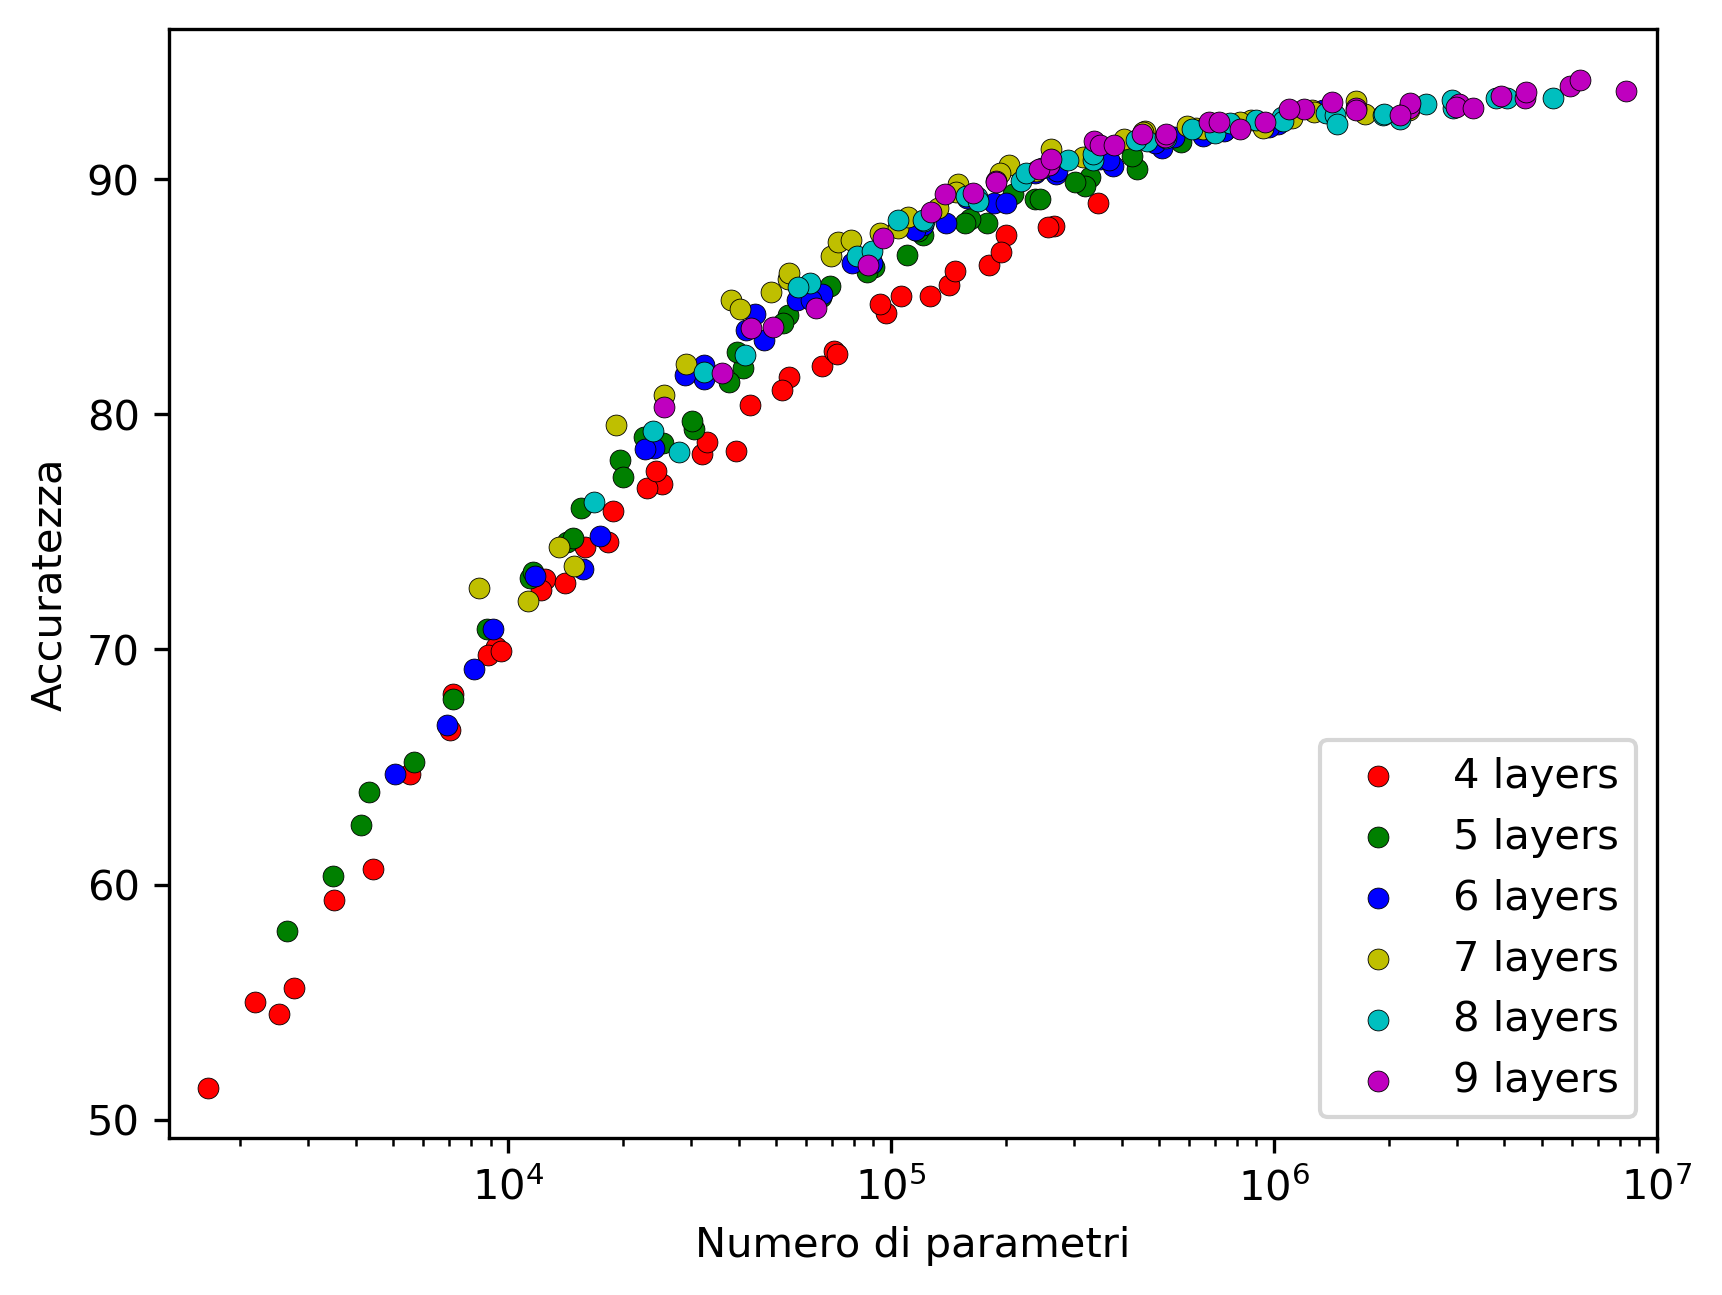
\includegraphics[width=0.3\textwidth]{tesi/immagini/dati_layer_log.png}}\quad
    \subfloat[]{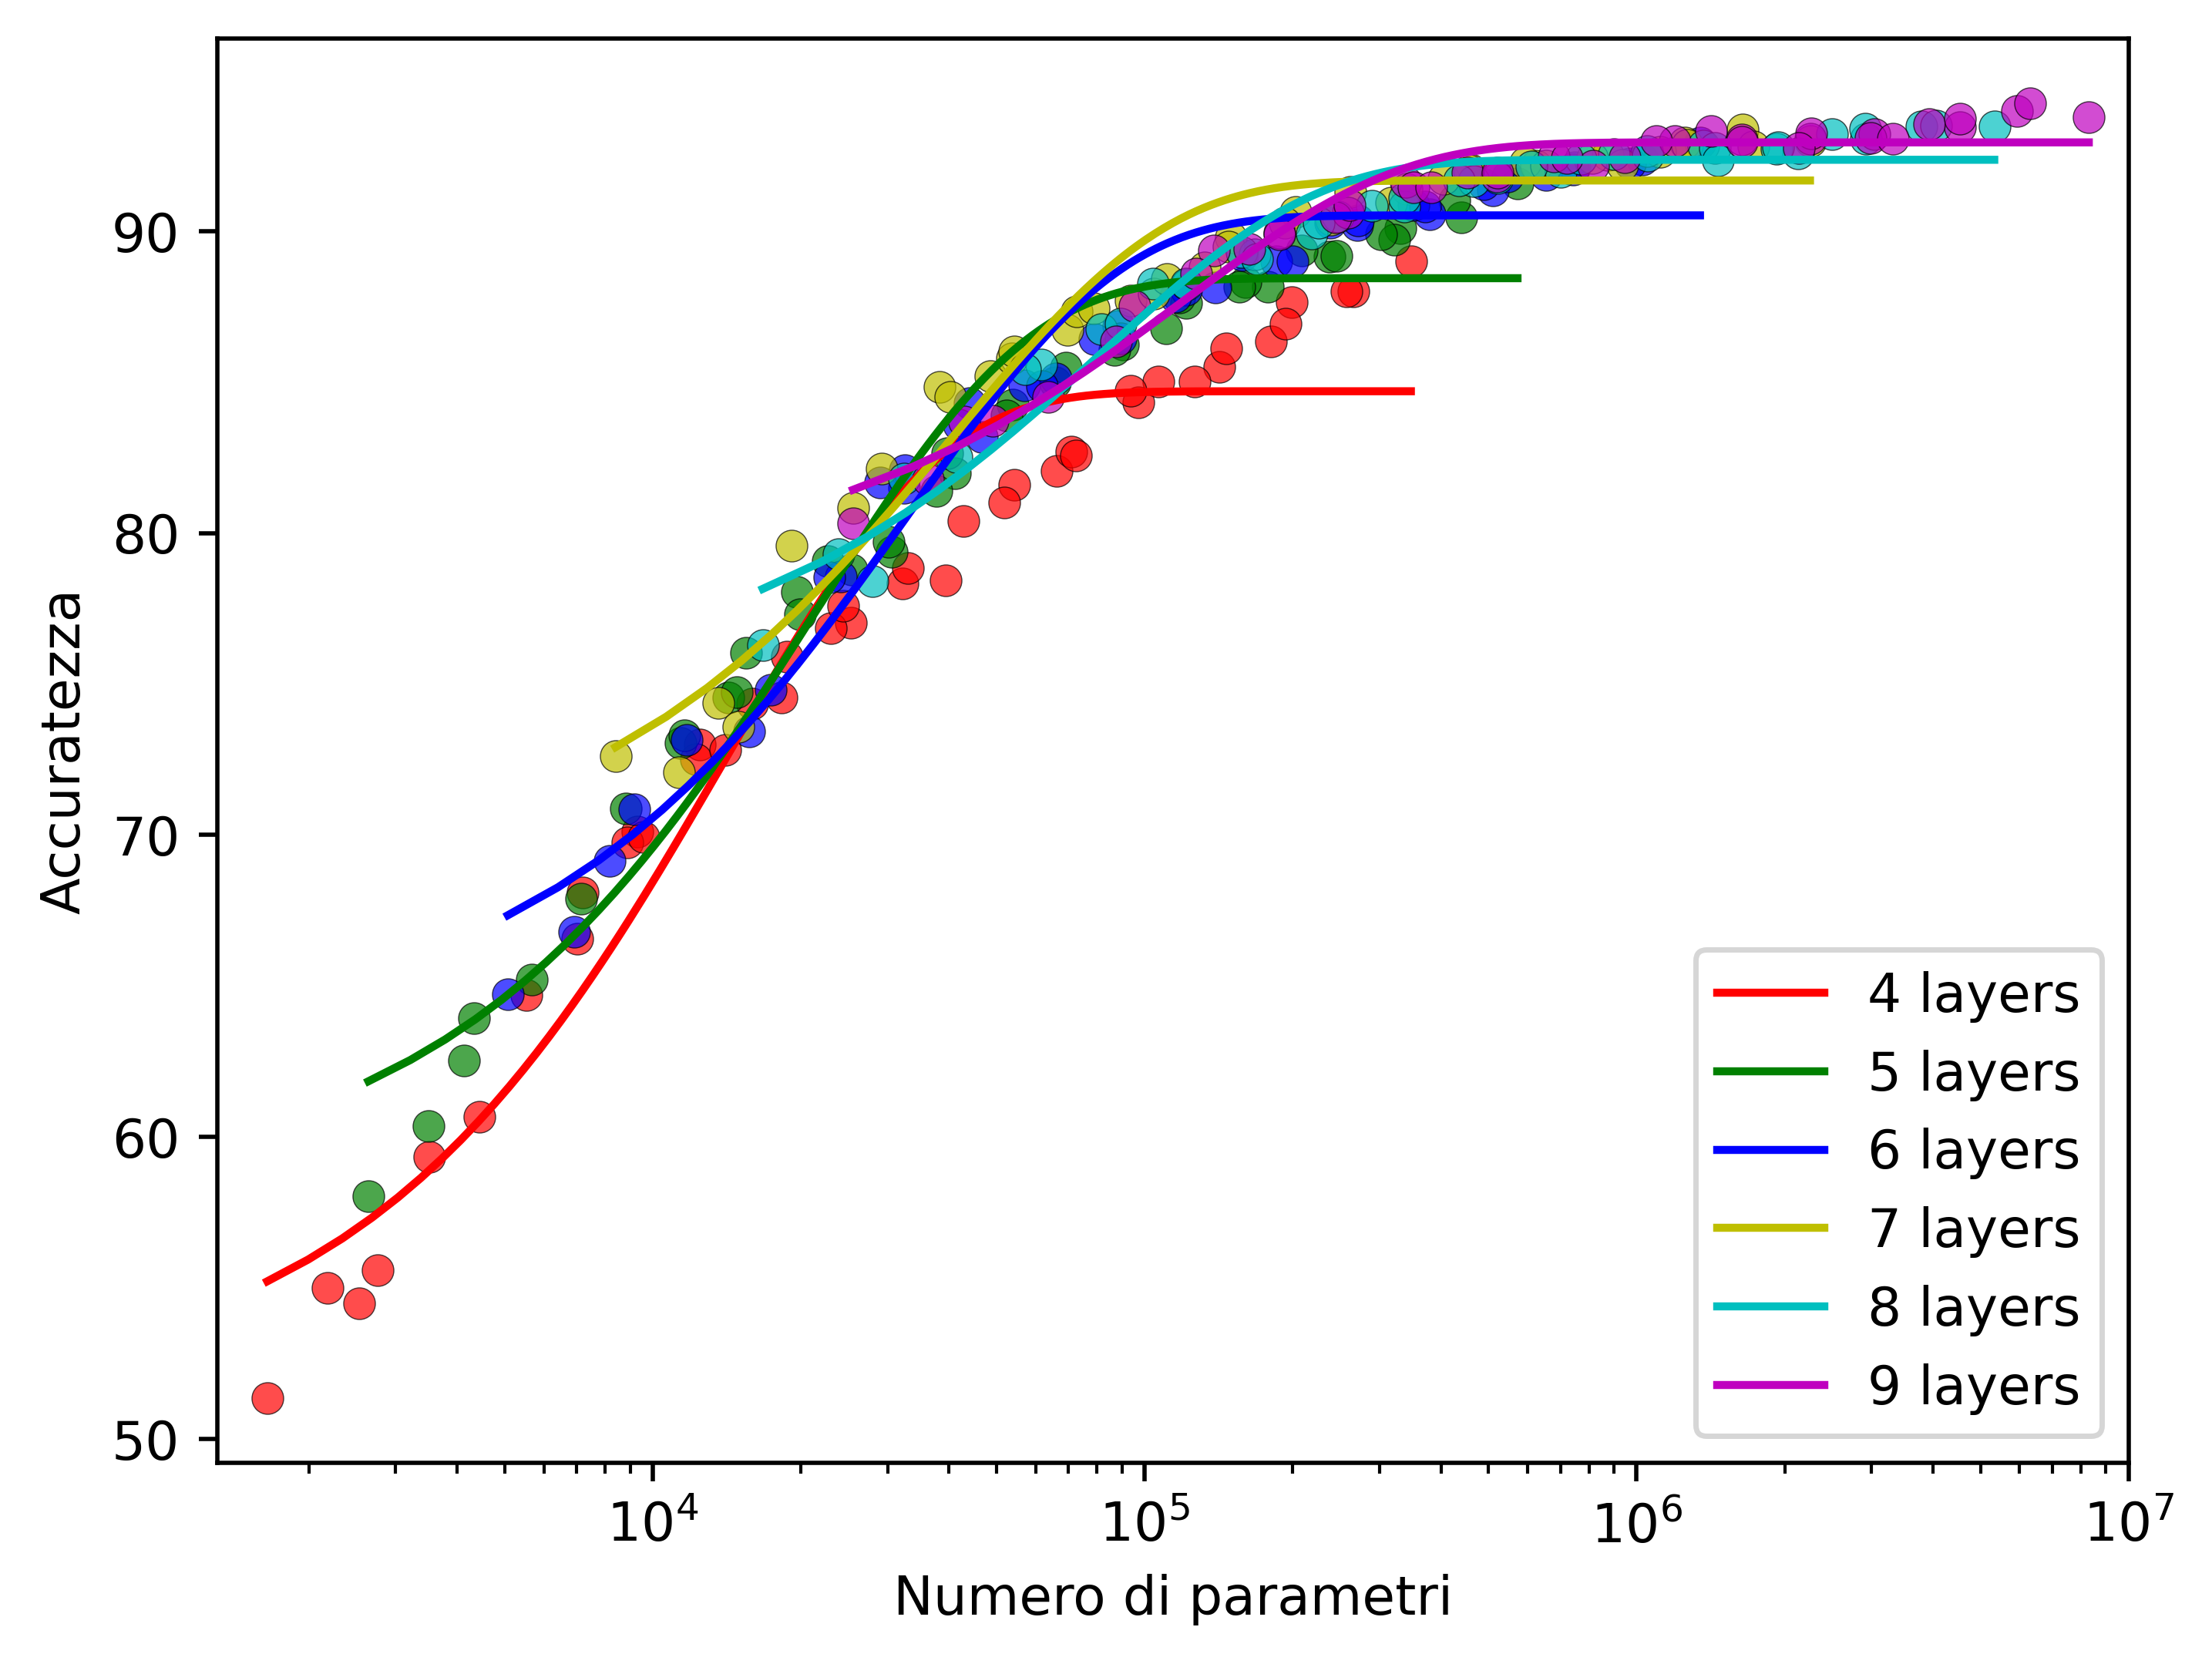
\includegraphics[width=0.3\textwidth]{tesi/immagini/exp_reg_log.png}}\quad
    \subfloat[]{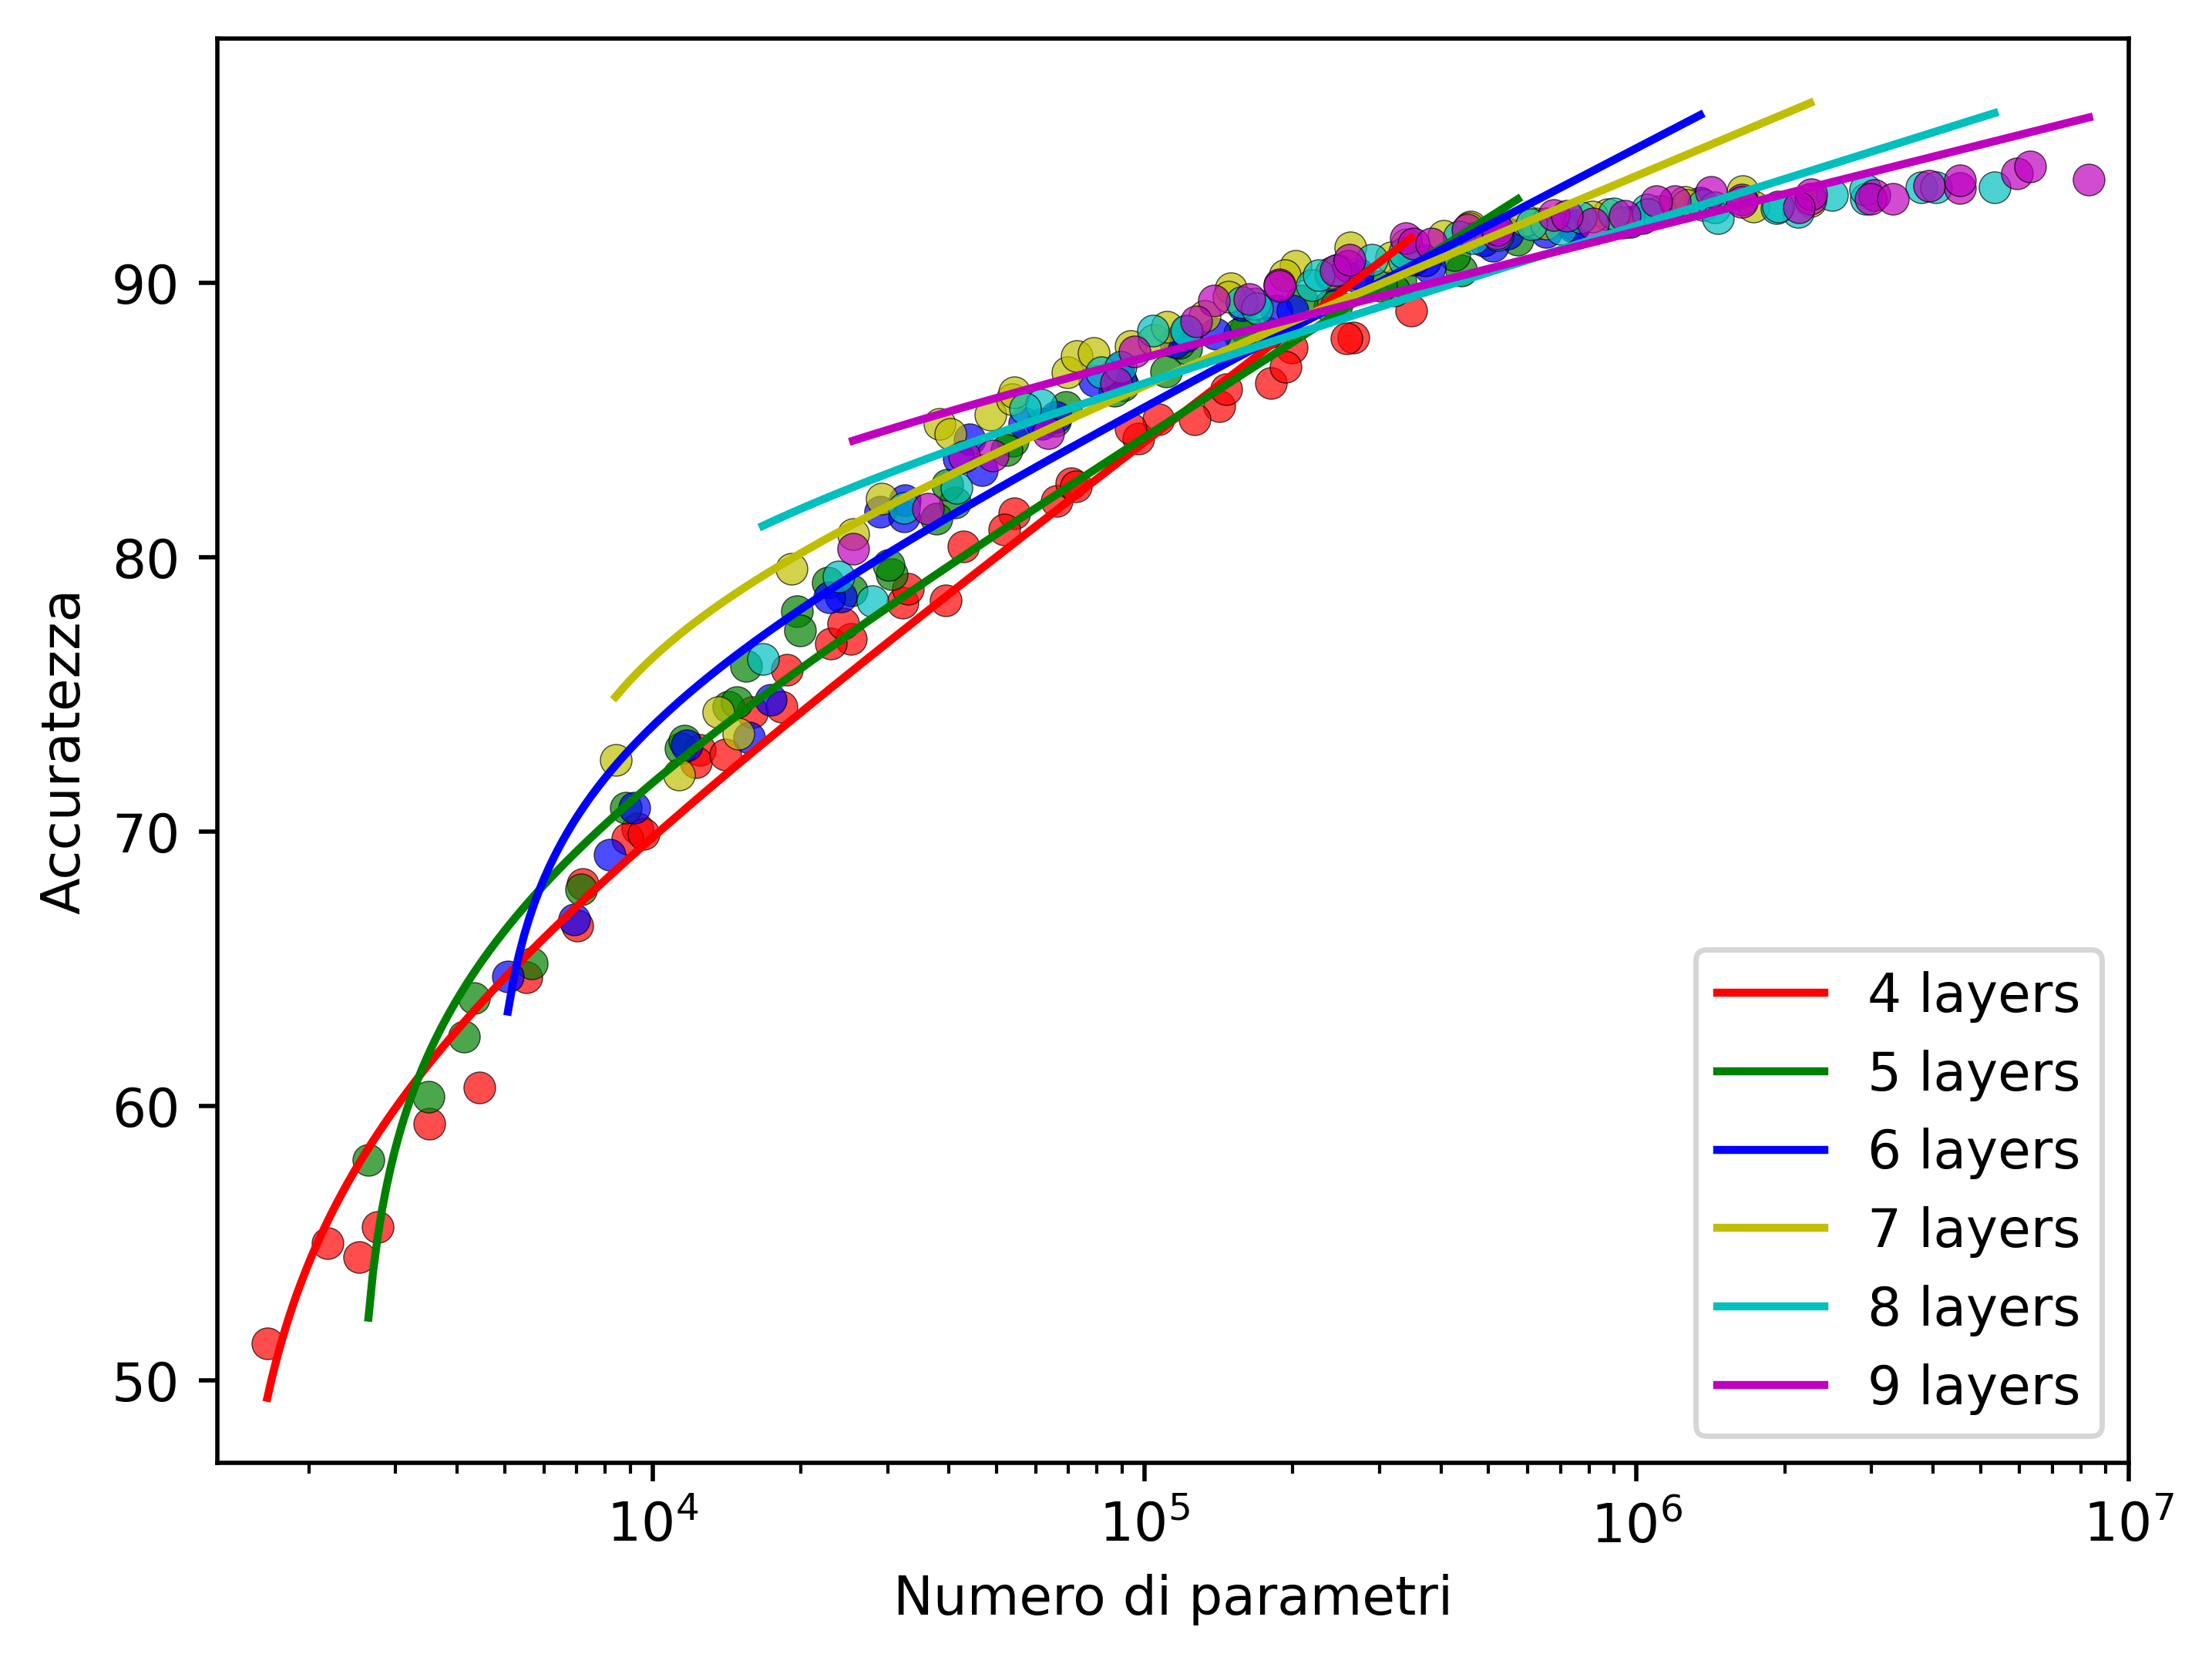
\includegraphics[width=0.3\textwidth]{tesi/immagini/log_reg_log.png}}\quad
    \subfloat[]{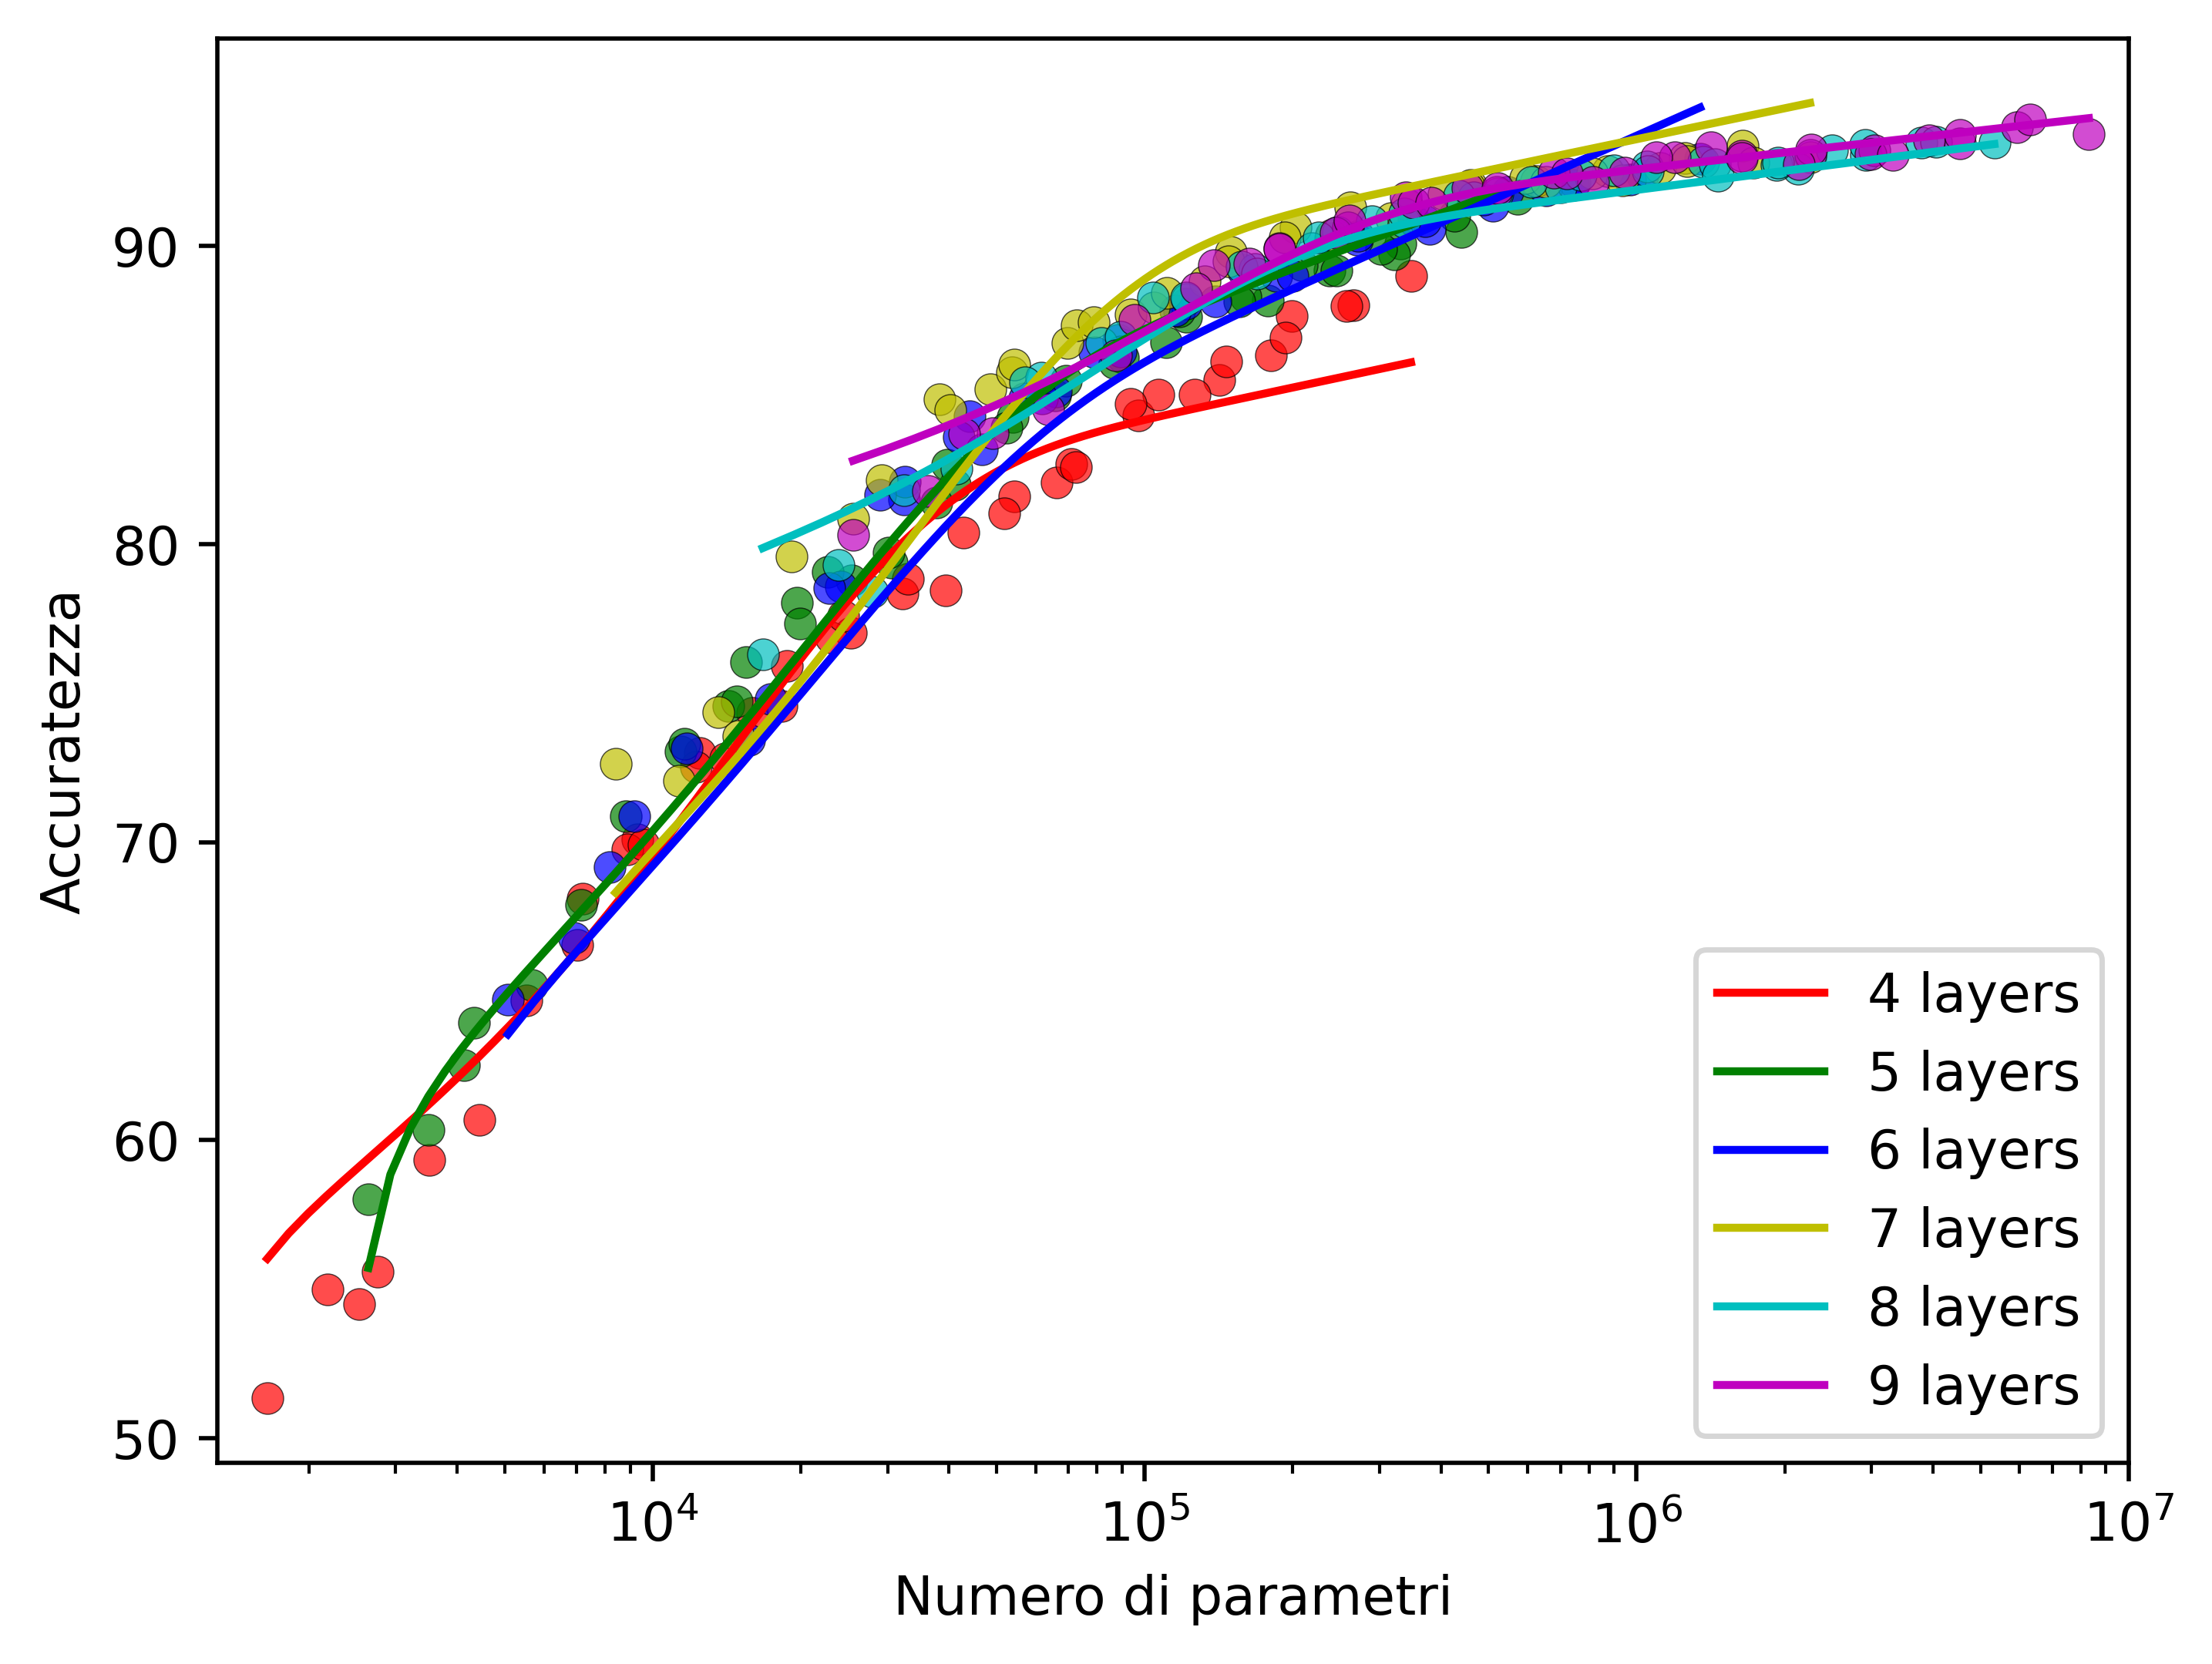
\includegraphics[width=0.3\textwidth]{tesi/immagini/comb_reg_log.png}}\quad
    \subfloat[]{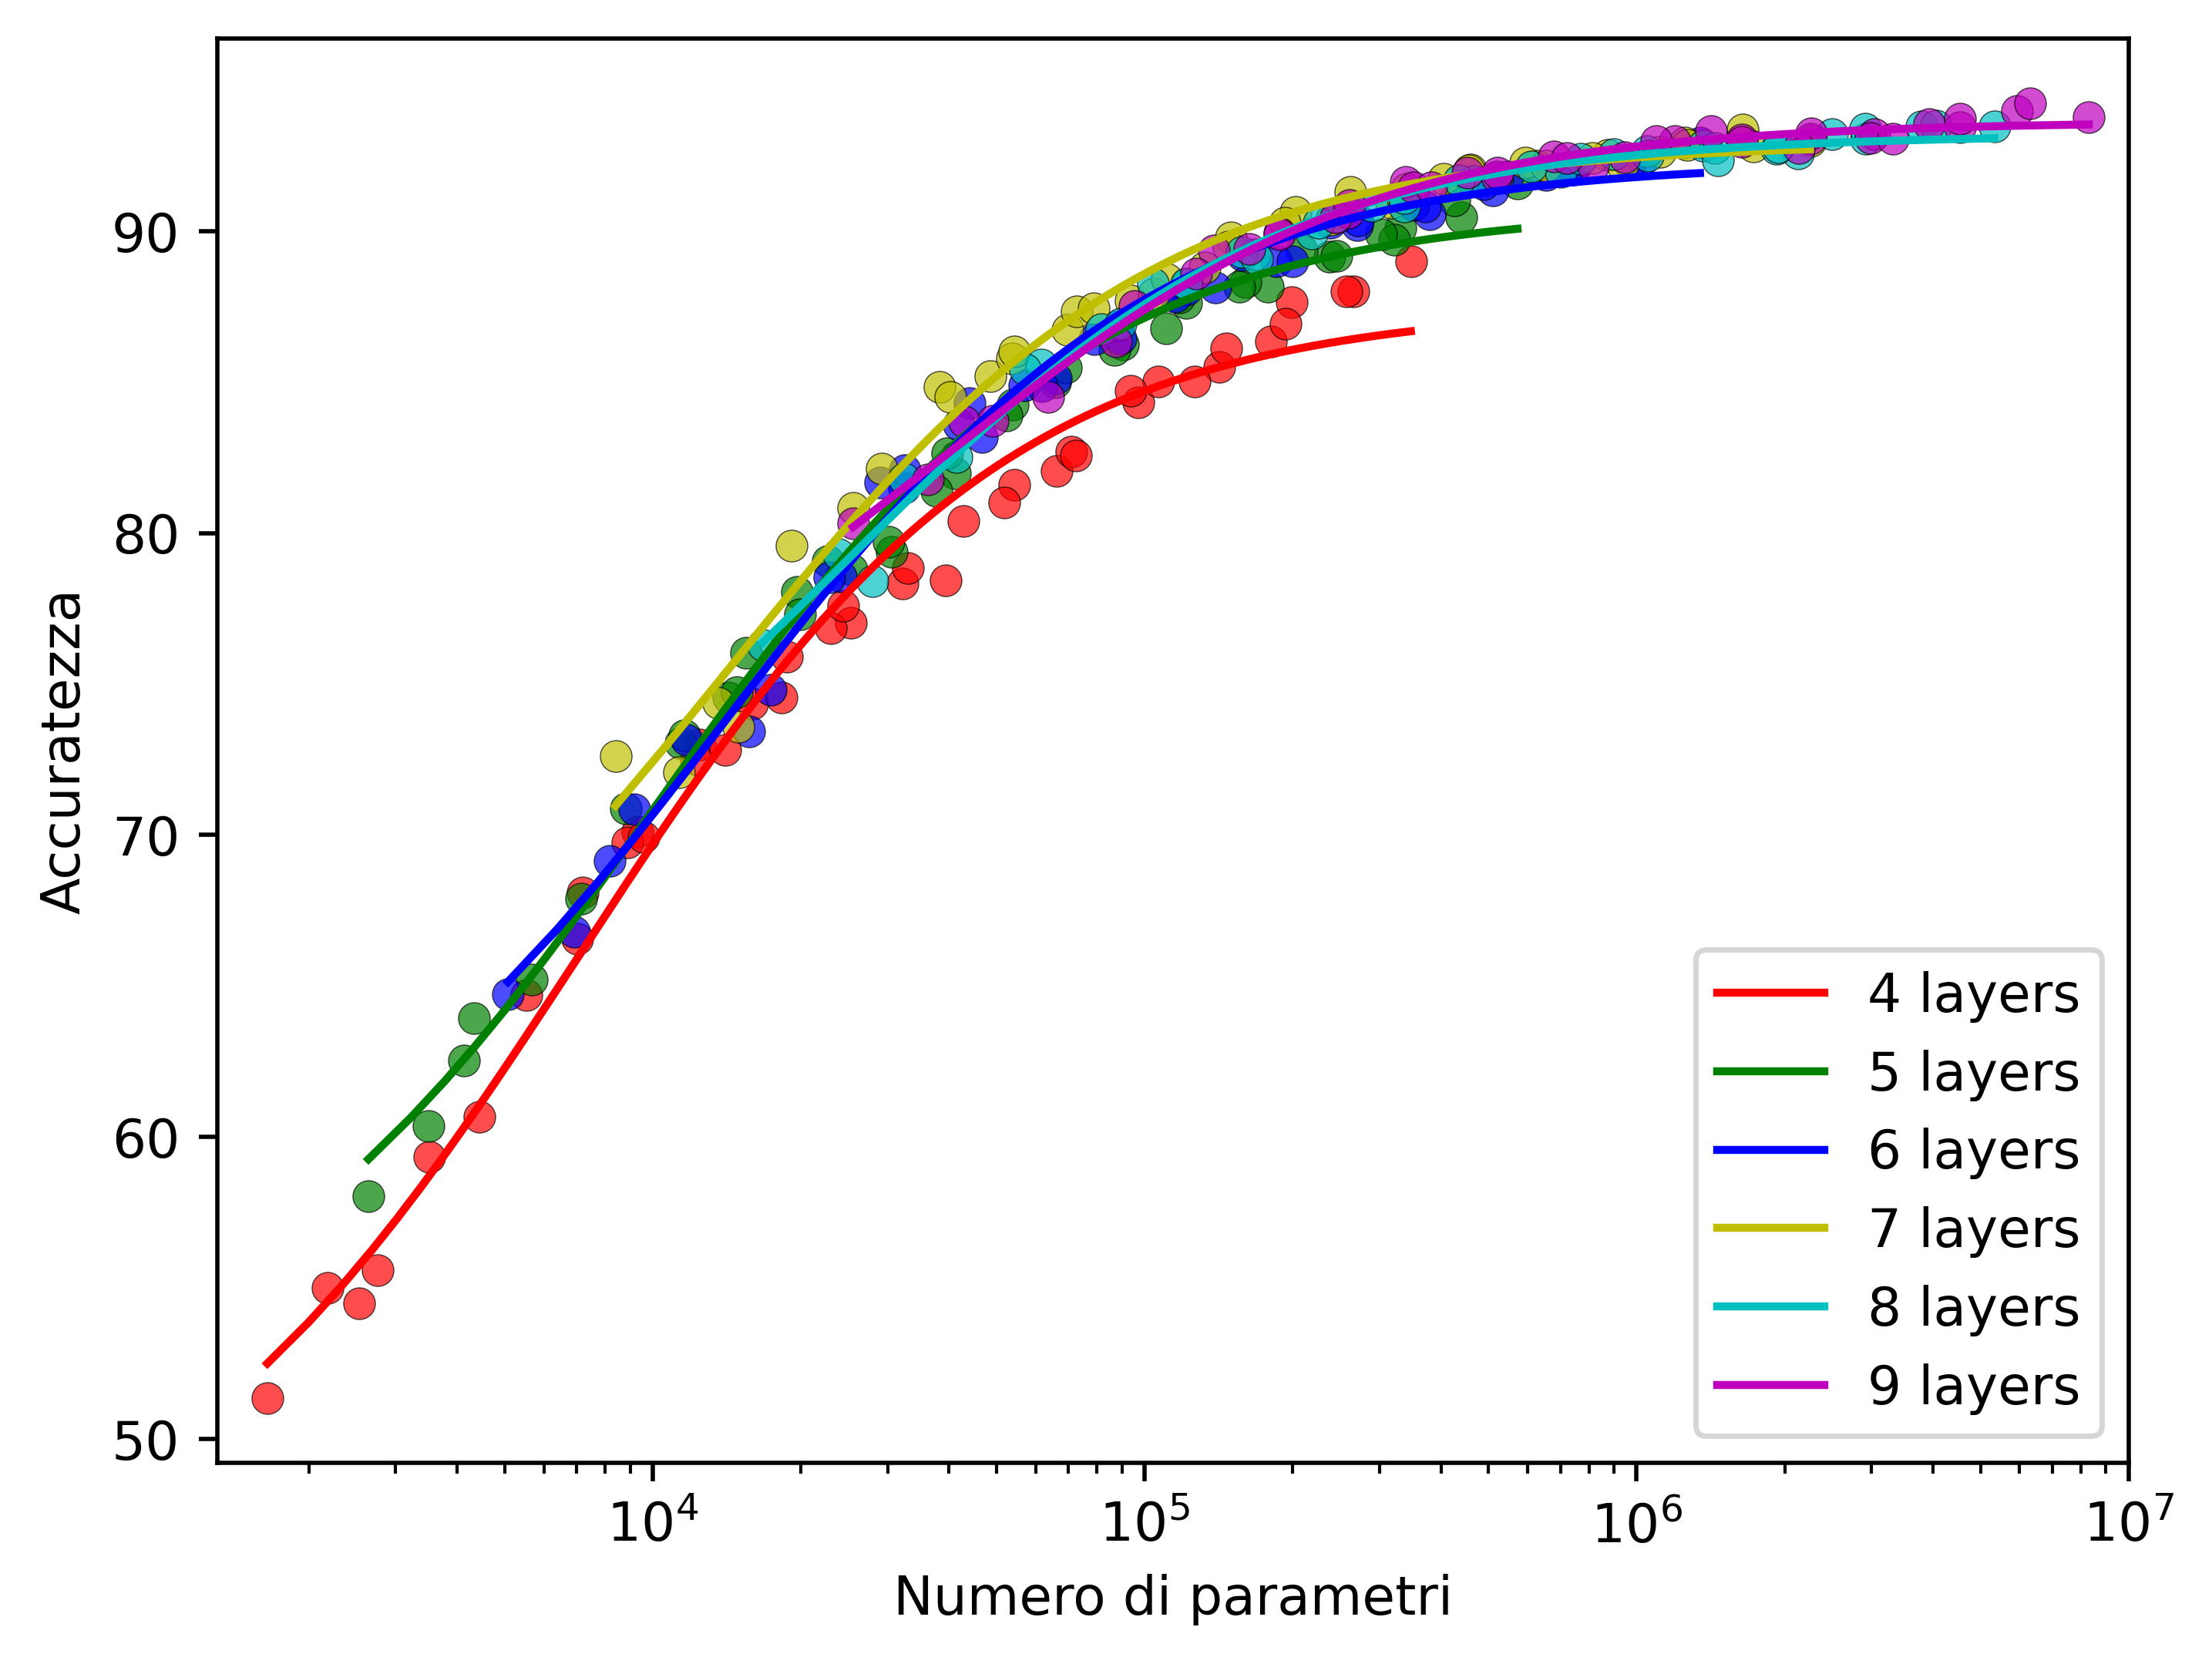
\includegraphics[width=0.3\textwidth]{tesi/immagini/hyp_reg_log.png}}\quad
    \subfloat[]{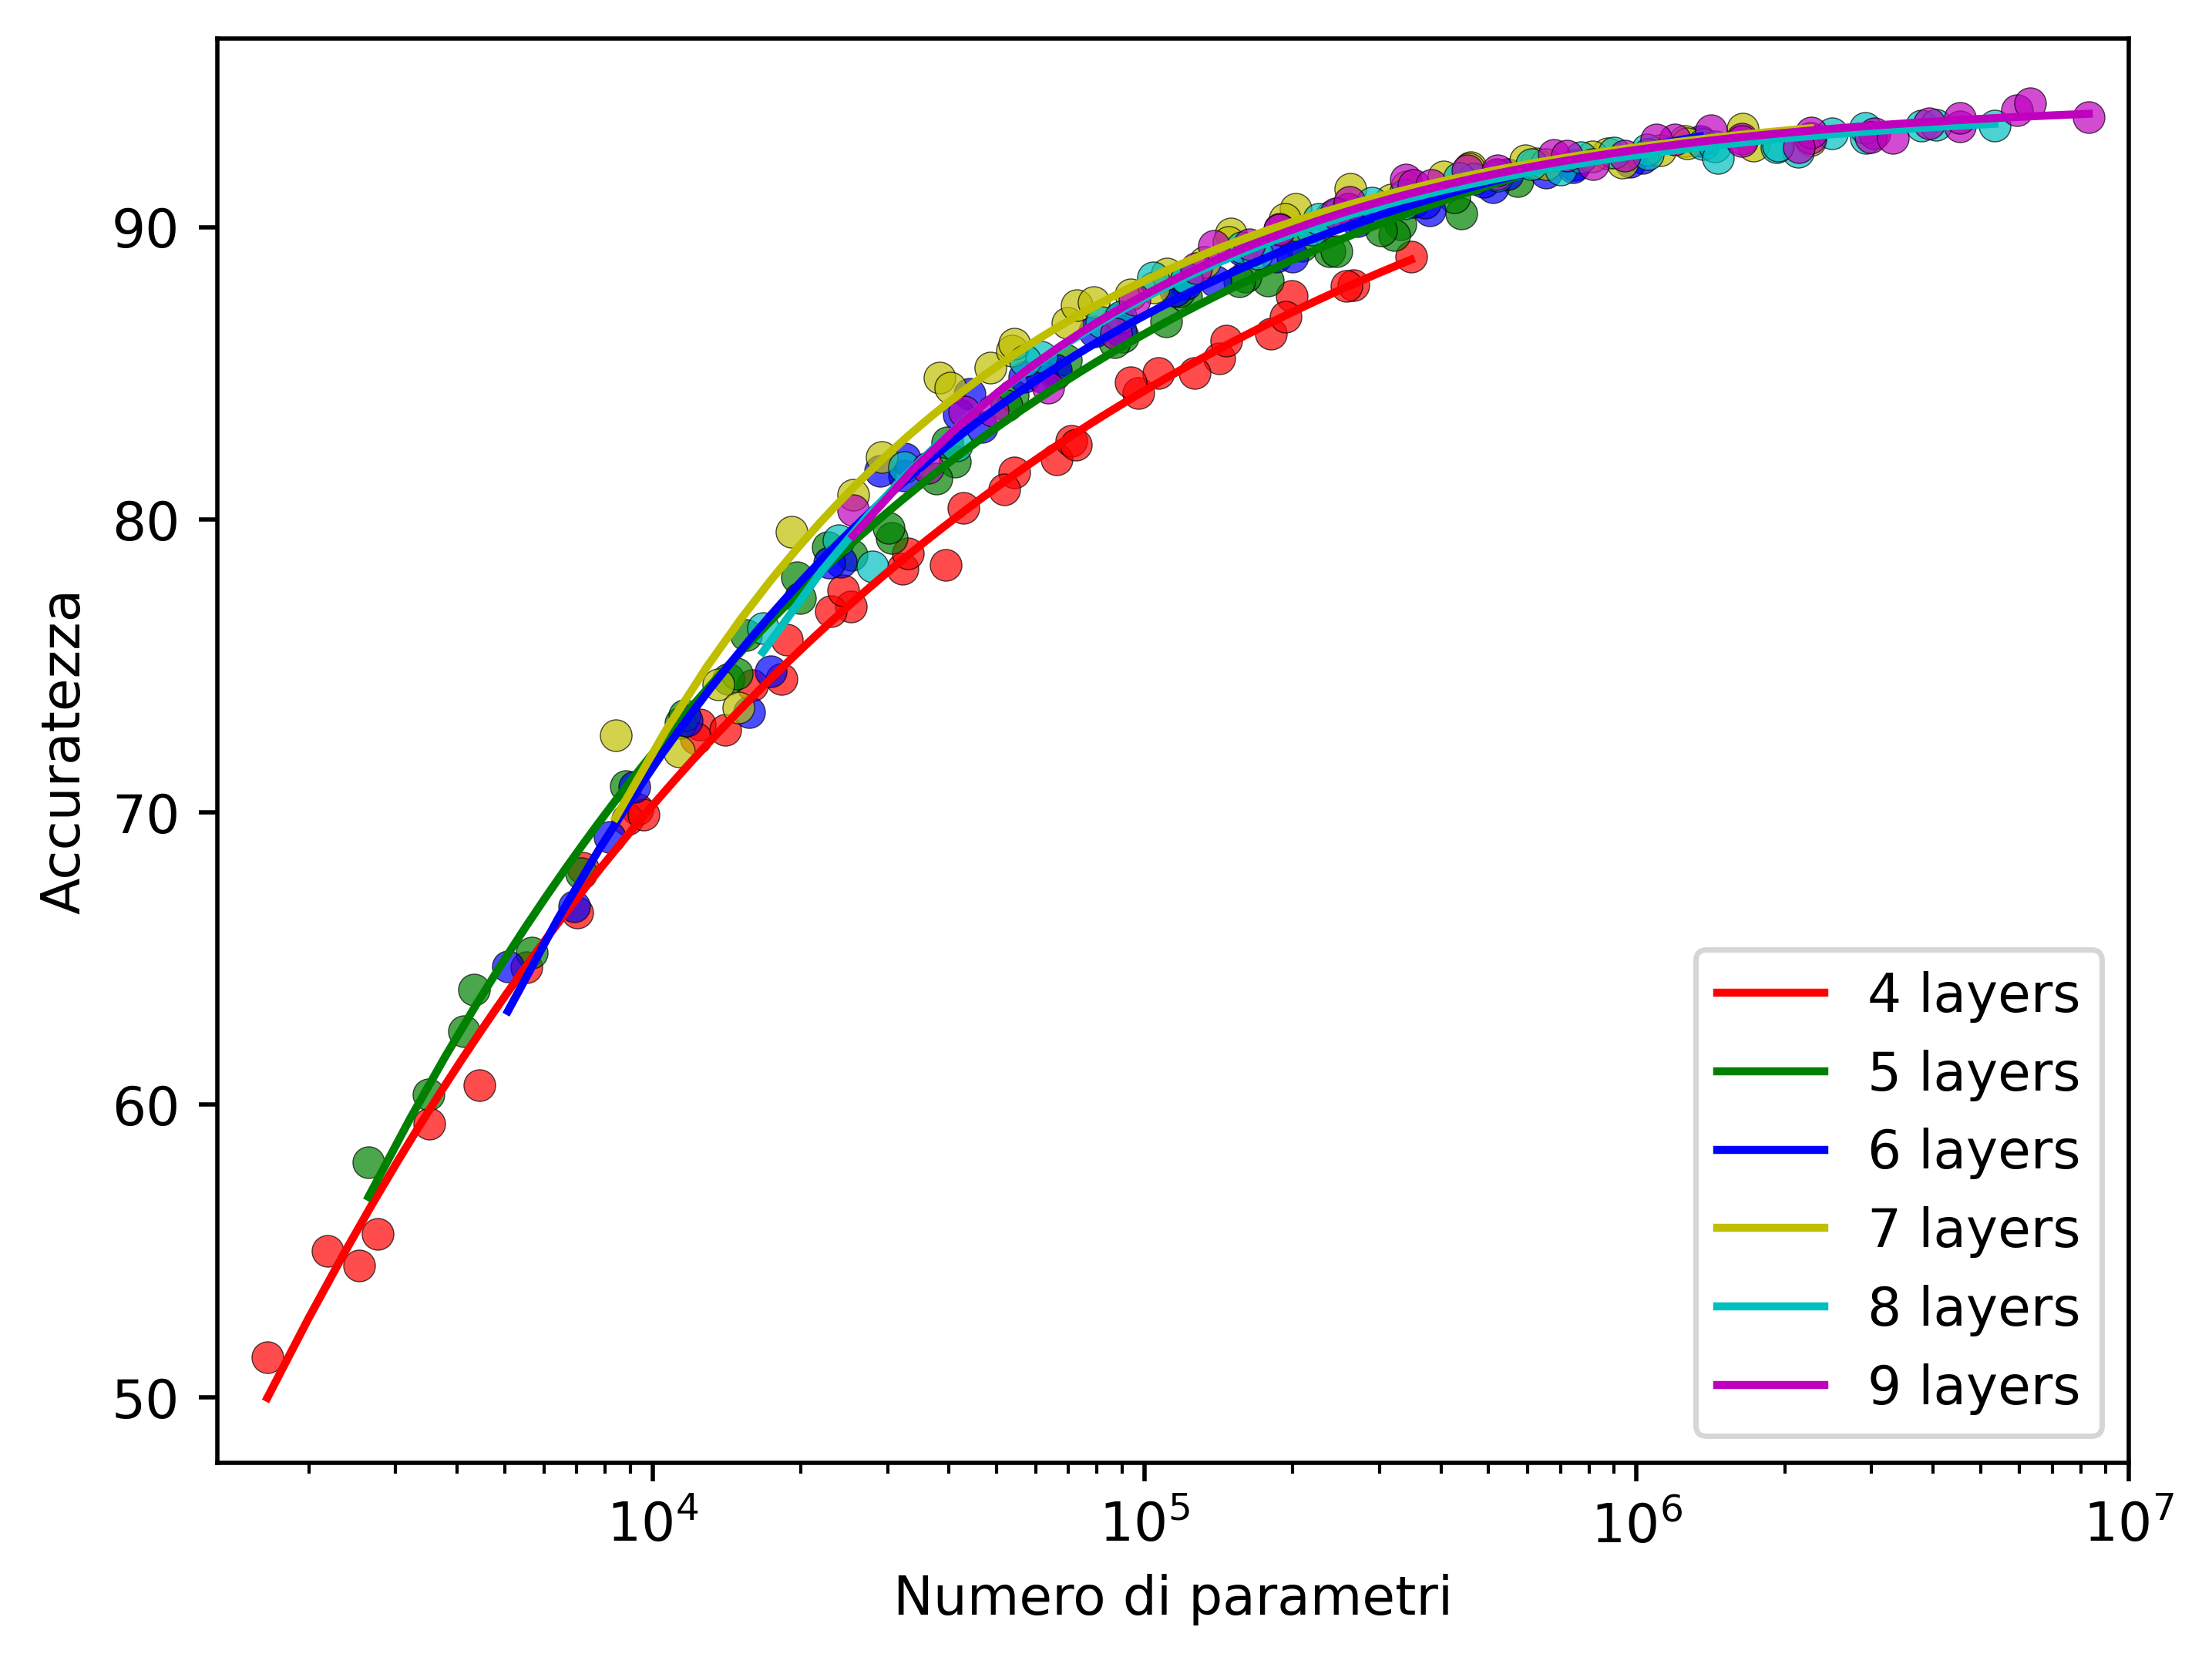
\includegraphics[width=0.3\textwidth]{tesi/immagini/hyp+_reg_log.png}}\quad
    \caption{\textit{Funzioni di regressione}. (a) Distribuzione dei dati raccolti, (b) regressione esponenziale, (c) regressione logaritmica, (d) combinazione convessa tra funzione logaritmica ed esponenziale, (e) regressione iperbolica, (f) regressione iperbolica generalizzata.}
    \label{fig:qualitativa}
\end{figure}

In figura \ref{fig:qualitativa} sono riportati gli andamenti delle funzioni di regressione testate, visualizzati sulla scala logaritmica per poter meglio apprezzare le differenze. 

Osservando qualitativamente risulta immediato notare come alcuni dei modelli di regressione proposti non approssimino bene l'andamento dei dati in possesso e non siano quindi utili per fornire una stima precisa dell'accuratezza di classificazione di una PhiNet. In particolare è chiaro come le funzioni presenti nei grafici (b), (c) e (d) non si adattino in maniera accettabile alle distribuzioni proposte.

D'altra parte entrambi i modelli di regressione (e) ed (f) non solo sembrano adattarsi bene ai dati raccolti, ma rispettano anche le intersezioni tra le curve distintive dei vari layers.

\subsection{Analisi quantitativa}

Ai fini di quantificare concretamente l'efficacia e l'accuratezza delle previsioni di tali modelli di regressione è necessario utilizzare delle metriche di valutazione che offrano una misura oggettiva delle loro prestazioni.
L'importanza di una corretta valutazione dei modelli di regressione risiede nel fatto che essa consente di identificare i punti di forza e di debolezza dei modelli (presenza o meno di asintoti verticali e/o orizzontali), nonché di effettuare confronti accurati tra diverse tecniche.

La metrica più comune per la valutazione di un modello di regressione è l'errore quadratico medio (o \textit{Root Mean Square Error}, RMSE), che, tramite il calcolo del quadrato della differenza tra il valore predetto e quello atteso, penalizza maggiormente la presenza di errori di previsione elevati rispetto ad esempio all'errore assoluto medio (MAE), che invece tiene in considerazione soltanto il valore assoluto della differenza in questione.

In questa analisi viene utilizzata per la valutazione del modello la metrica del RMSE, calcolata su modelli di regressione ottenuti osservando solamente un sottoinsieme ridotto della totalità dei dati originariamente disponibili, tramite la tecnica della \textit{cross-validation}.

Questa metodologia di valutazione della validazione incrociata consente di ottenere metriche affidabili per il confronto tra modelli di regressione in quanto ogni modello viene valutato (ed addestrato) su diverse combinazioni di dati. La tecnica della \textit{cross-validation} consiste in un iniziale suddivisione dei dati a disposizione in diversi \textit{fold}, ovvero insiemi equipotenti che si distinguono tra loro per le diverse partizioni dei dati tra set di addestramento e set di test. In questo modo si ottengono $K$ insiemi contenenti gli stessi dati ma che si distinguono per la diversa suddivisione delle informazioni tra i vari set. Per ogni \textit{fold} viene allenato il modello di regressione sul rispettivo set di addestramento e valutato, tramite il calcolo delle metriche scelte, sul set di test; l'intero processo viene ripetuto per ogni \textit{fold} disponibile ($K$ volte) in modo da garantire una valutazione affidabile e non influenzata da eventuali outlier.

Nel caso in questione, dato che si ottengono 6 diverse funzioni di regressioni (una per ogni valore diverso di numero di layer) verrà applicata la tecnica di cross-validation altrettante volte, calcolando l'errore quadratico medio per ogni valore di numero di layer. In particolare i dati a disposizione sono stati suddivisi in $K=500$ fold equipotenti, ognuno partizionato in maniera differente mantenendo però le proporzioni di 70\%-30\% tra il set di addestramento e quello di test.

La procedura inizia quindi con la creazione dei 500 fold, riordinati randomicamente, per ogni insieme di dati appartenenti ad uno specifico valore di numero di layer. Per ciascun fold viene calcolata la funzione che meglio si adatta al set di addestramento tramite l'allenamento del modello di regressione scelto e viene successivamente eseguita la valutazione sul set di test. In questo modo per ogni fold differente si ottiene un valore di errore quadratico medio che verrà mediato con quello di tutti i $K$ fold generati. Ciò permette di ottenere un valore medio dei RMSE per ogni valore differente di numero di layer per un dato modello di regressione. La metrica finale utilizzata per il confronto è quindi la media degli errori quadratici medi per ogni funzione che approssima gli andamenti dei dati distribuiti sui vari layer.

In questa analisi i modelli di regressione che sembravano adattarsi meglio alla distribuzione di dati sono la regressione iperbolica e la sua generalizzazione. I calcoli delle metriche confermano che la funzione iperbolica generalizzata sia caratterizzata da una misura di errore inferiore rispetto alla semplice funzione iperbolica, per quest'ultima si ottiene infatti un valore medio dei RMSE di $0.807$\%, mentre il modello iperbolico ottimizzato riduce l'errore del 6\% facendolo attestare ad un valore di $0.758$\%. In entrambi i casi, l'errore ottenuto può essere assimilato a una statistica che descrive l'incertezza del processo di training.


\section{Smoothing}

Come si può notare dalla figura \ref{fig:segmentation} (a), la segmentazione ottenuta è molto rumorosa, soggetta ed outliers ed influenzata dal fatto di avere solamente un numero discreto di dati. 
Per rendere il tutto più semplice ed efficace da visualizzare viene utilizzato quindi un processo di \textit{smoothing} dei dati, che va ad eliminare dai segmenti ottenuti tutti quelli la cui ampiezza sta sotto ad una certa soglia, detta \textit{threshold}, e ricostruisce gli intervalli rimanenti. In questa situazione come ``ampiezza" si intende il logaritmo in base 10 che ha come argomento il rapporto tra l'estremo superiore e quello inferiore del segmento; in particolare la threshold utilizzata assume il valore di $threshold=0.13$ ed un intervallo verrà quindi considerato da scartare quando $log_{10}\left(\frac{estremo\ superiore}{estremo\ inferiore} \right) < threshold$.
Il risultato finale ottenuto sulla distribuzione di dati originaria è quindi visibile in figura \ref{fig:segmentation} (b), mentre quello ottenuto tramite la sola funzione di regressione (che non ha bisogno di alcun processo di smoothing) è mostrato in figura \ref{fig:segmentation} (c).

\begin{figure}[ht]
    \centering
    \subfloat[]{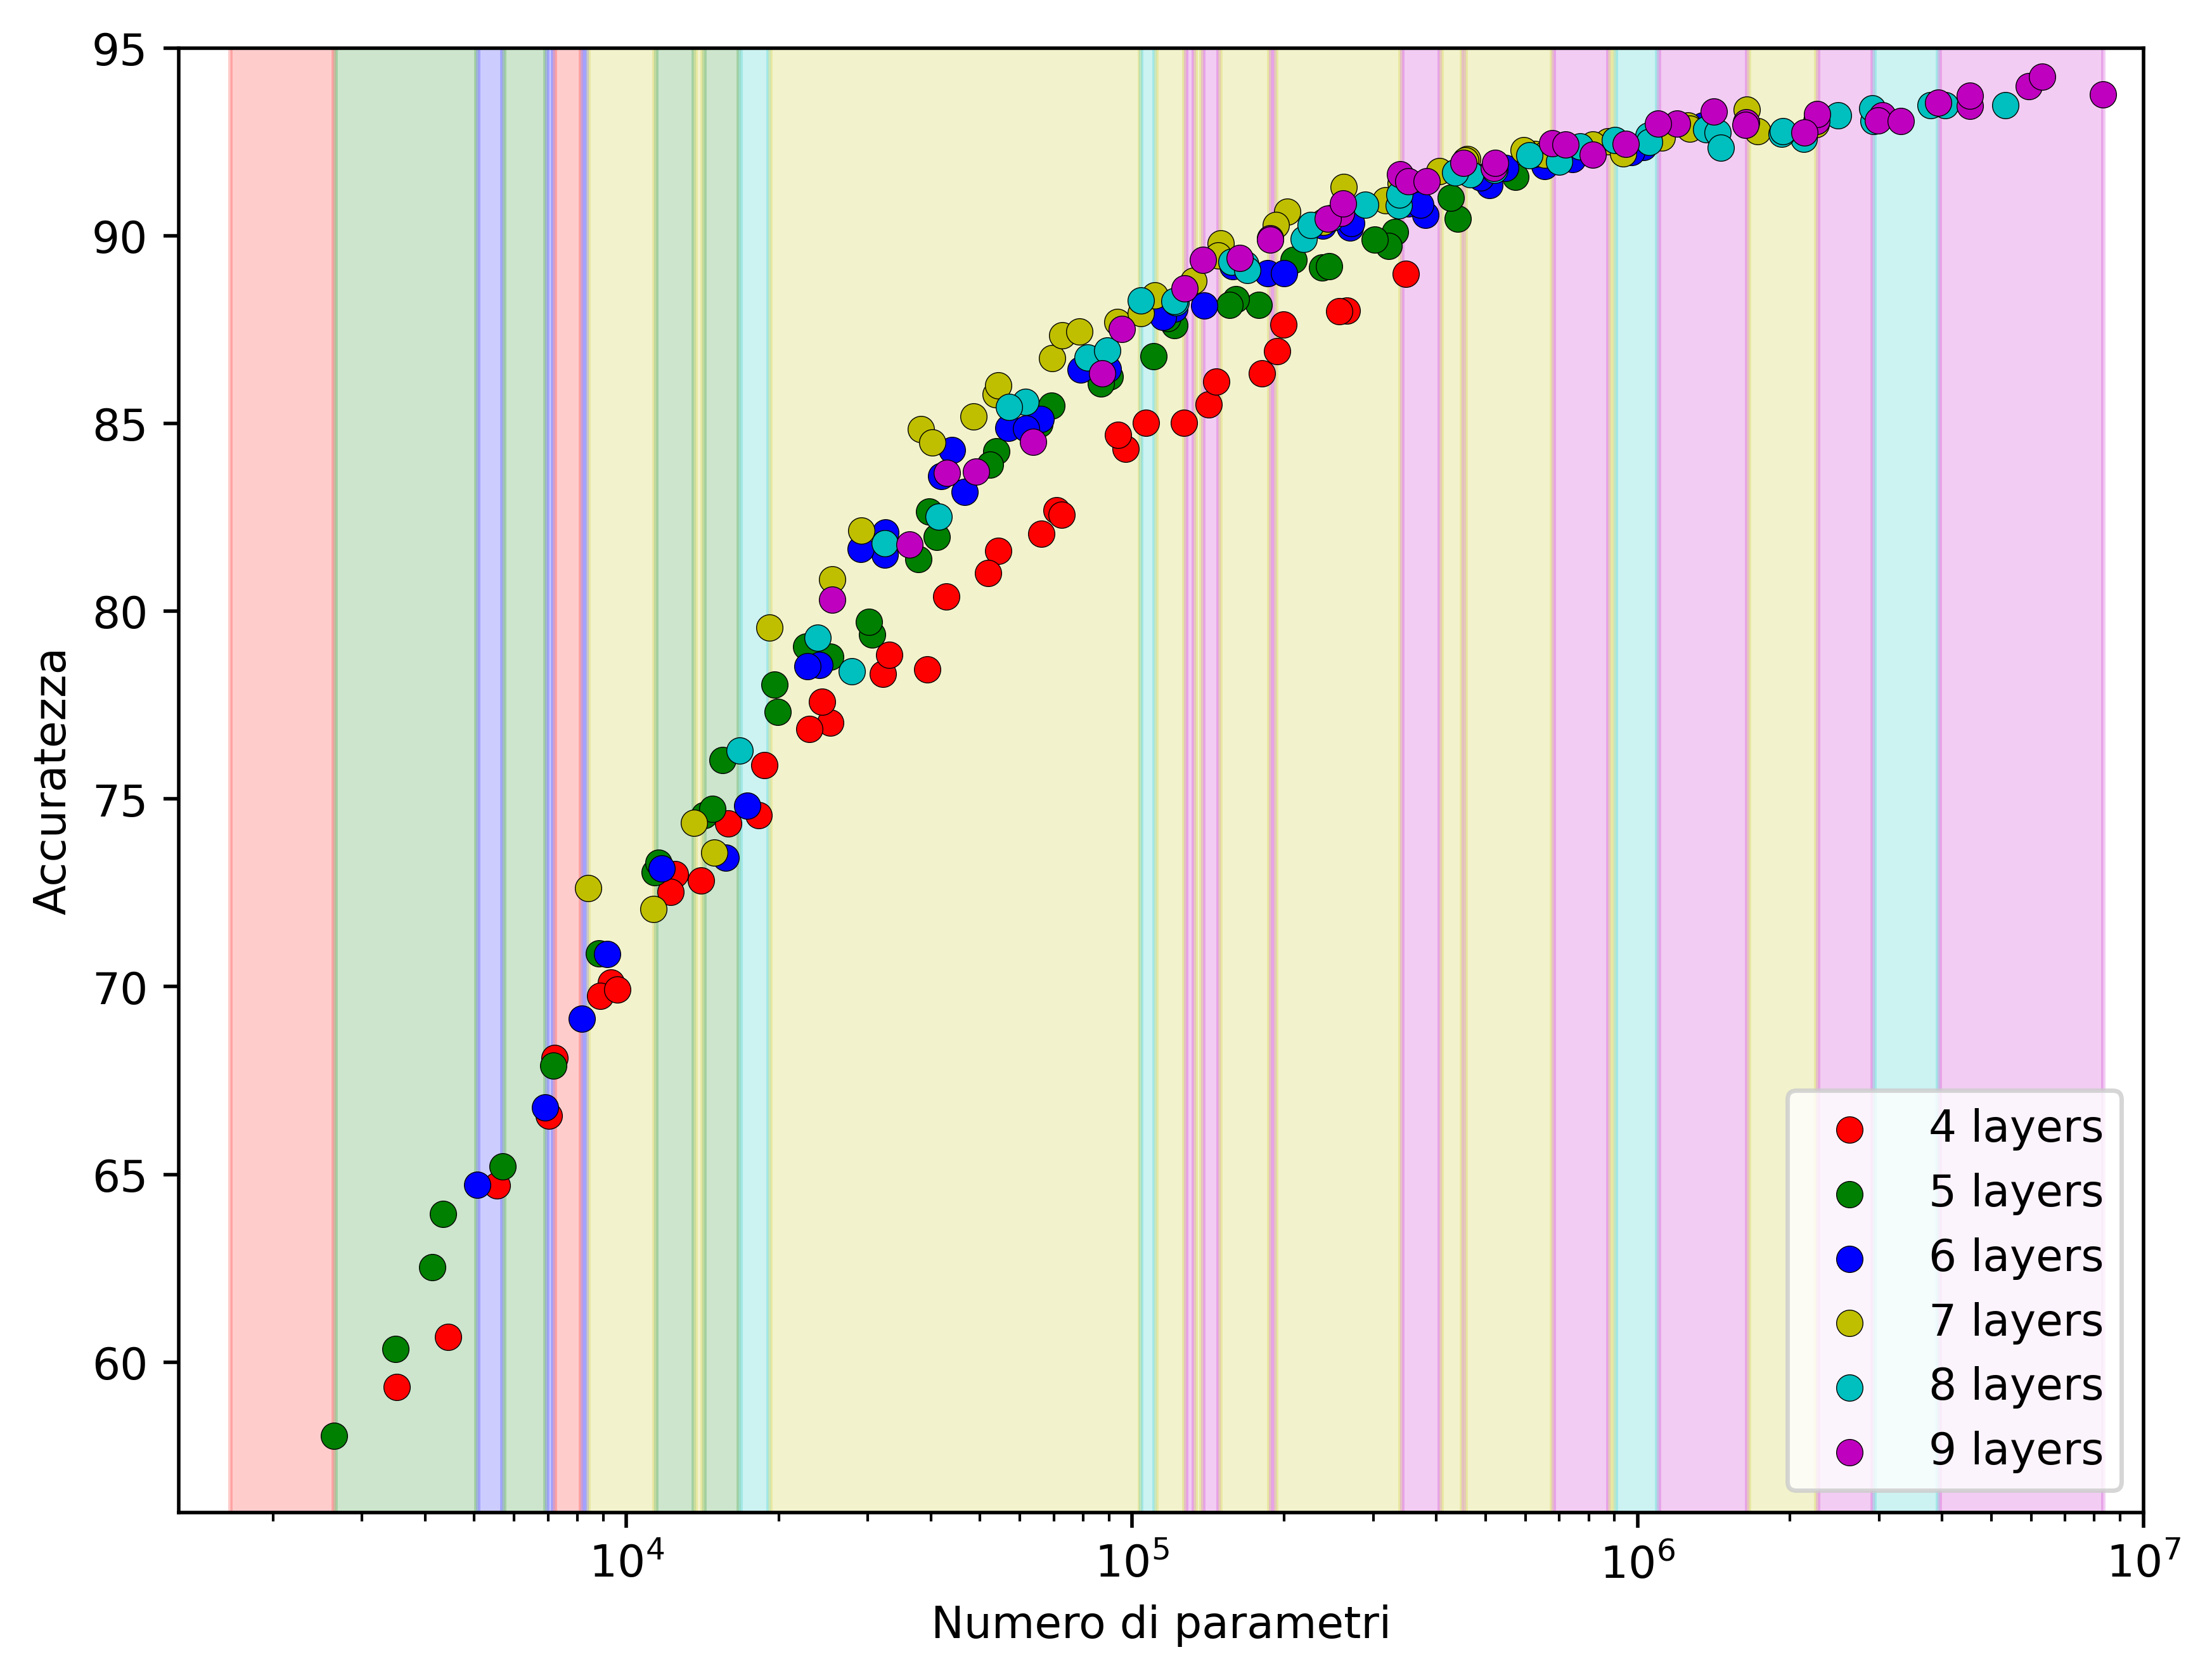
\includegraphics[width=0.31\textwidth]{tesi/immagini/segment_dati.png}}\quad
    \subfloat[]{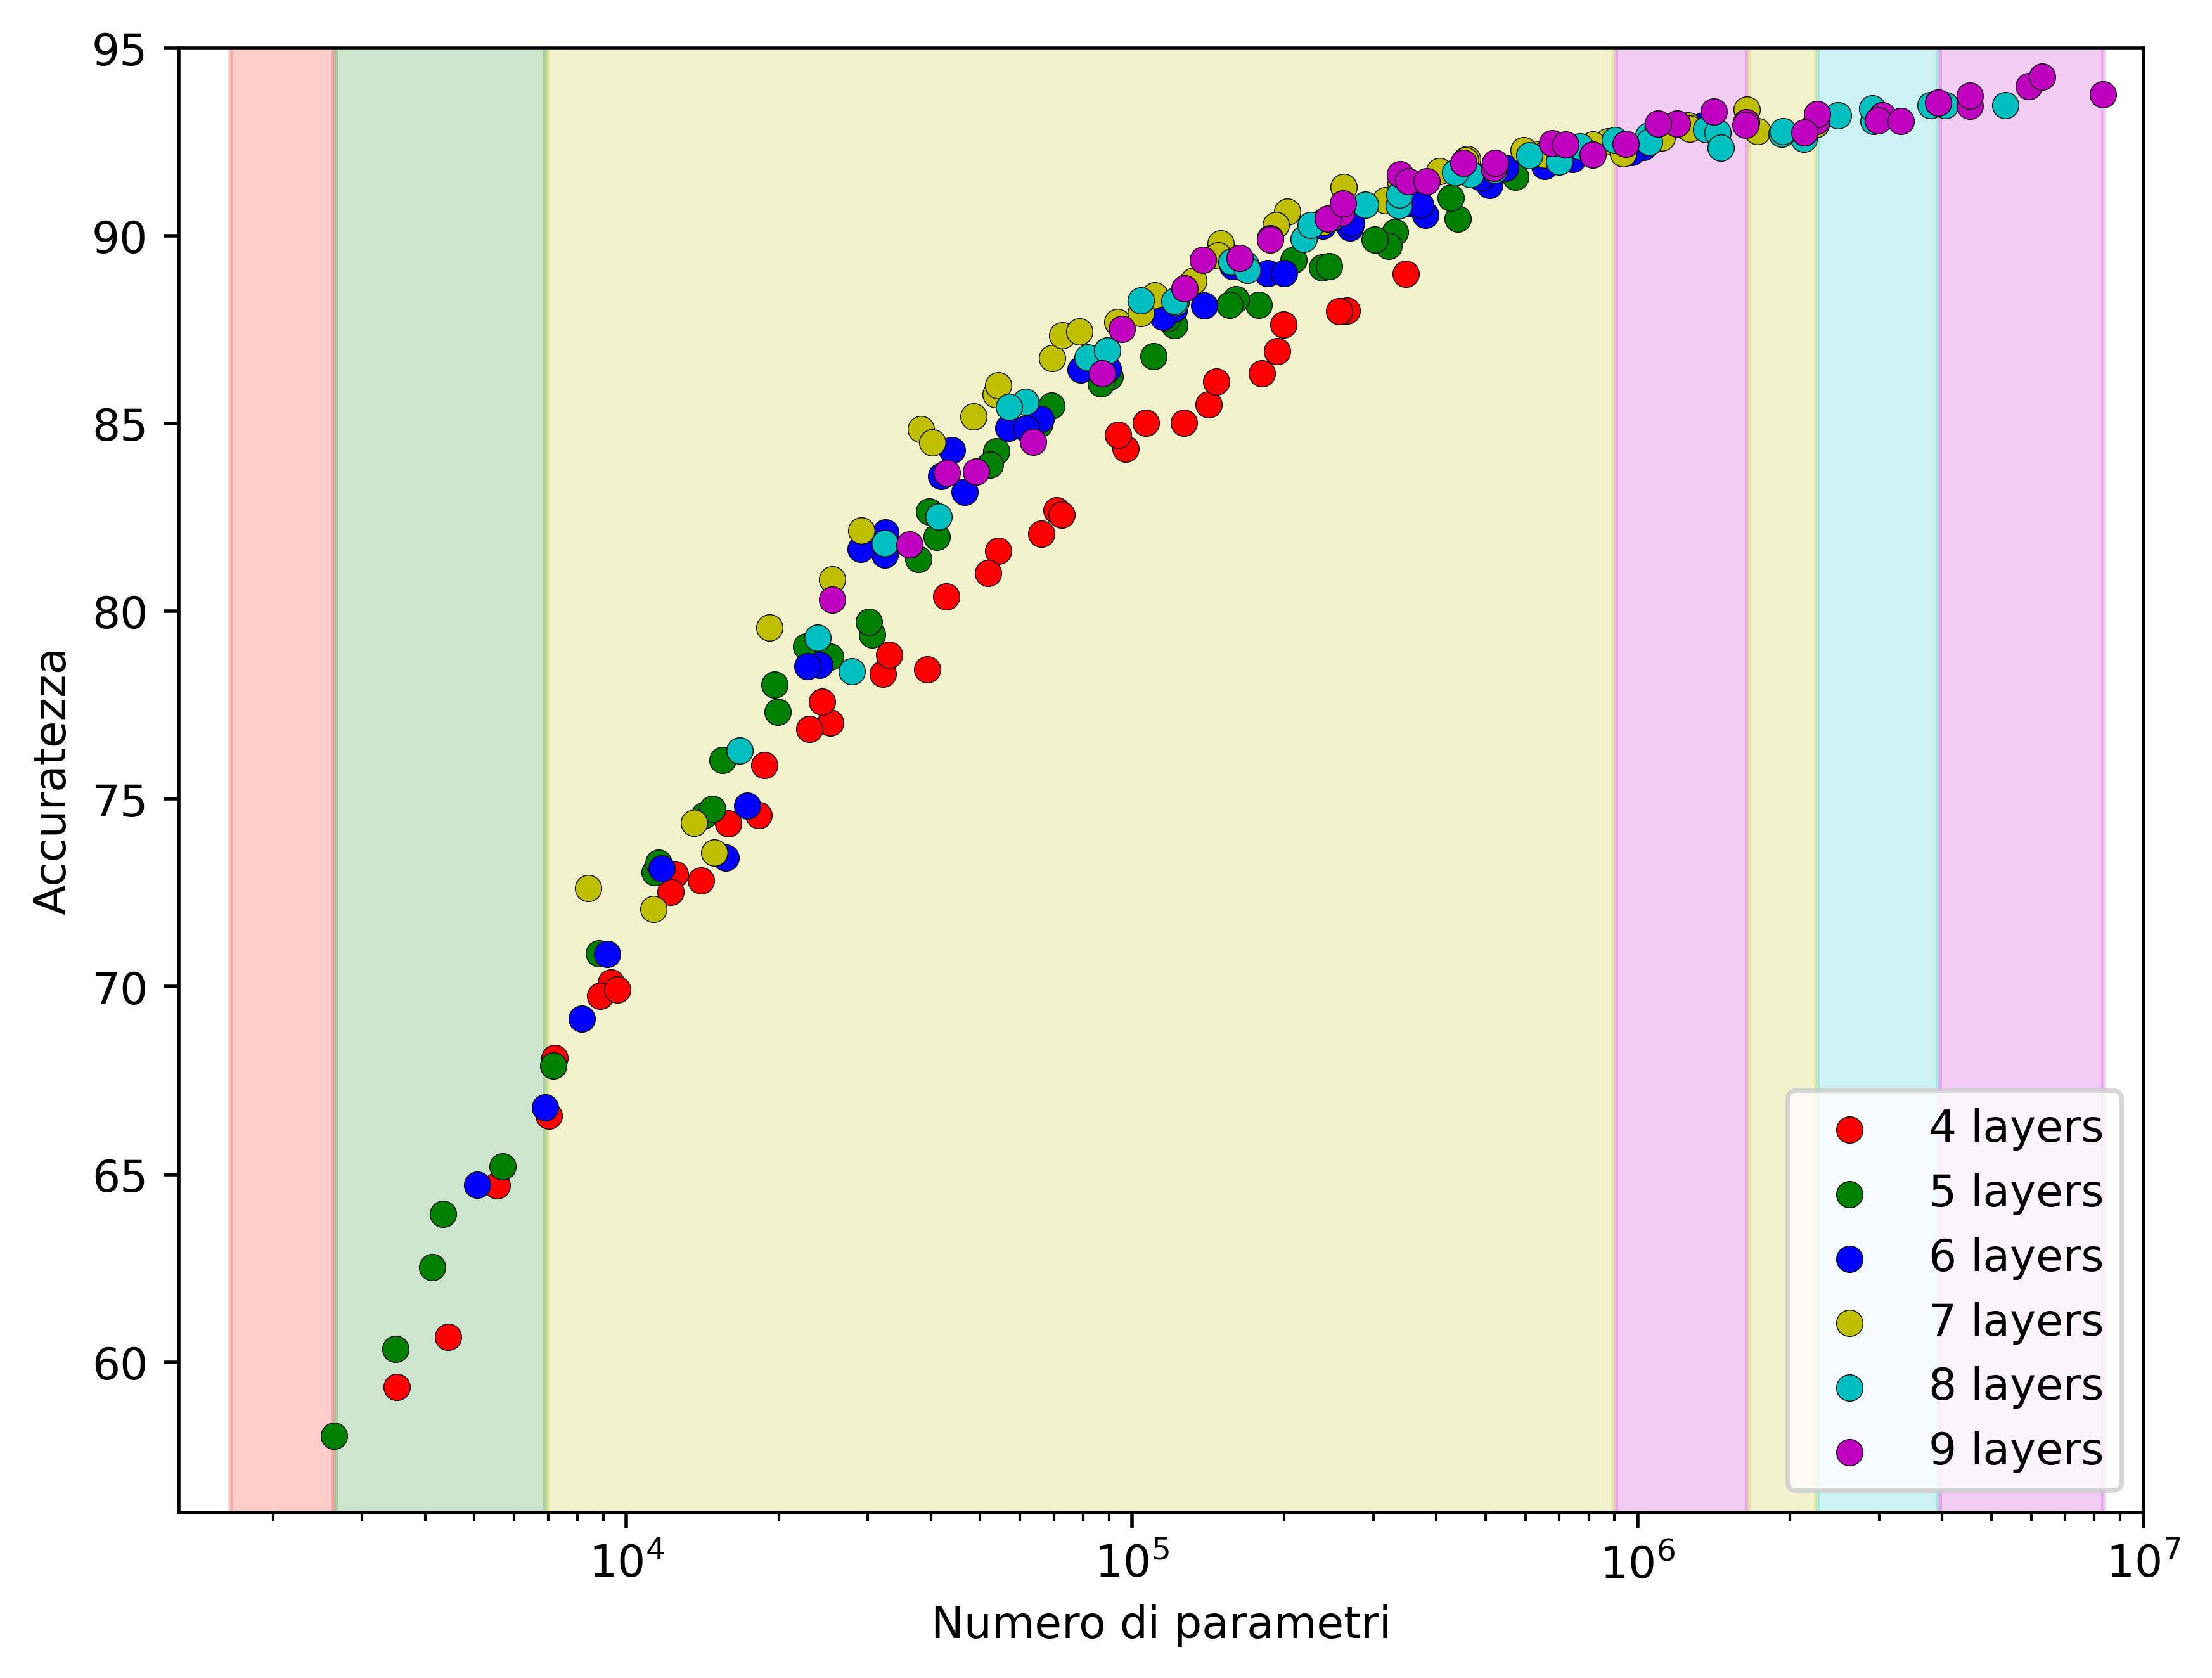
\includegraphics[width=0.31\textwidth]{tesi/immagini/segment_dati_smooth.png}}\quad
    \subfloat[]{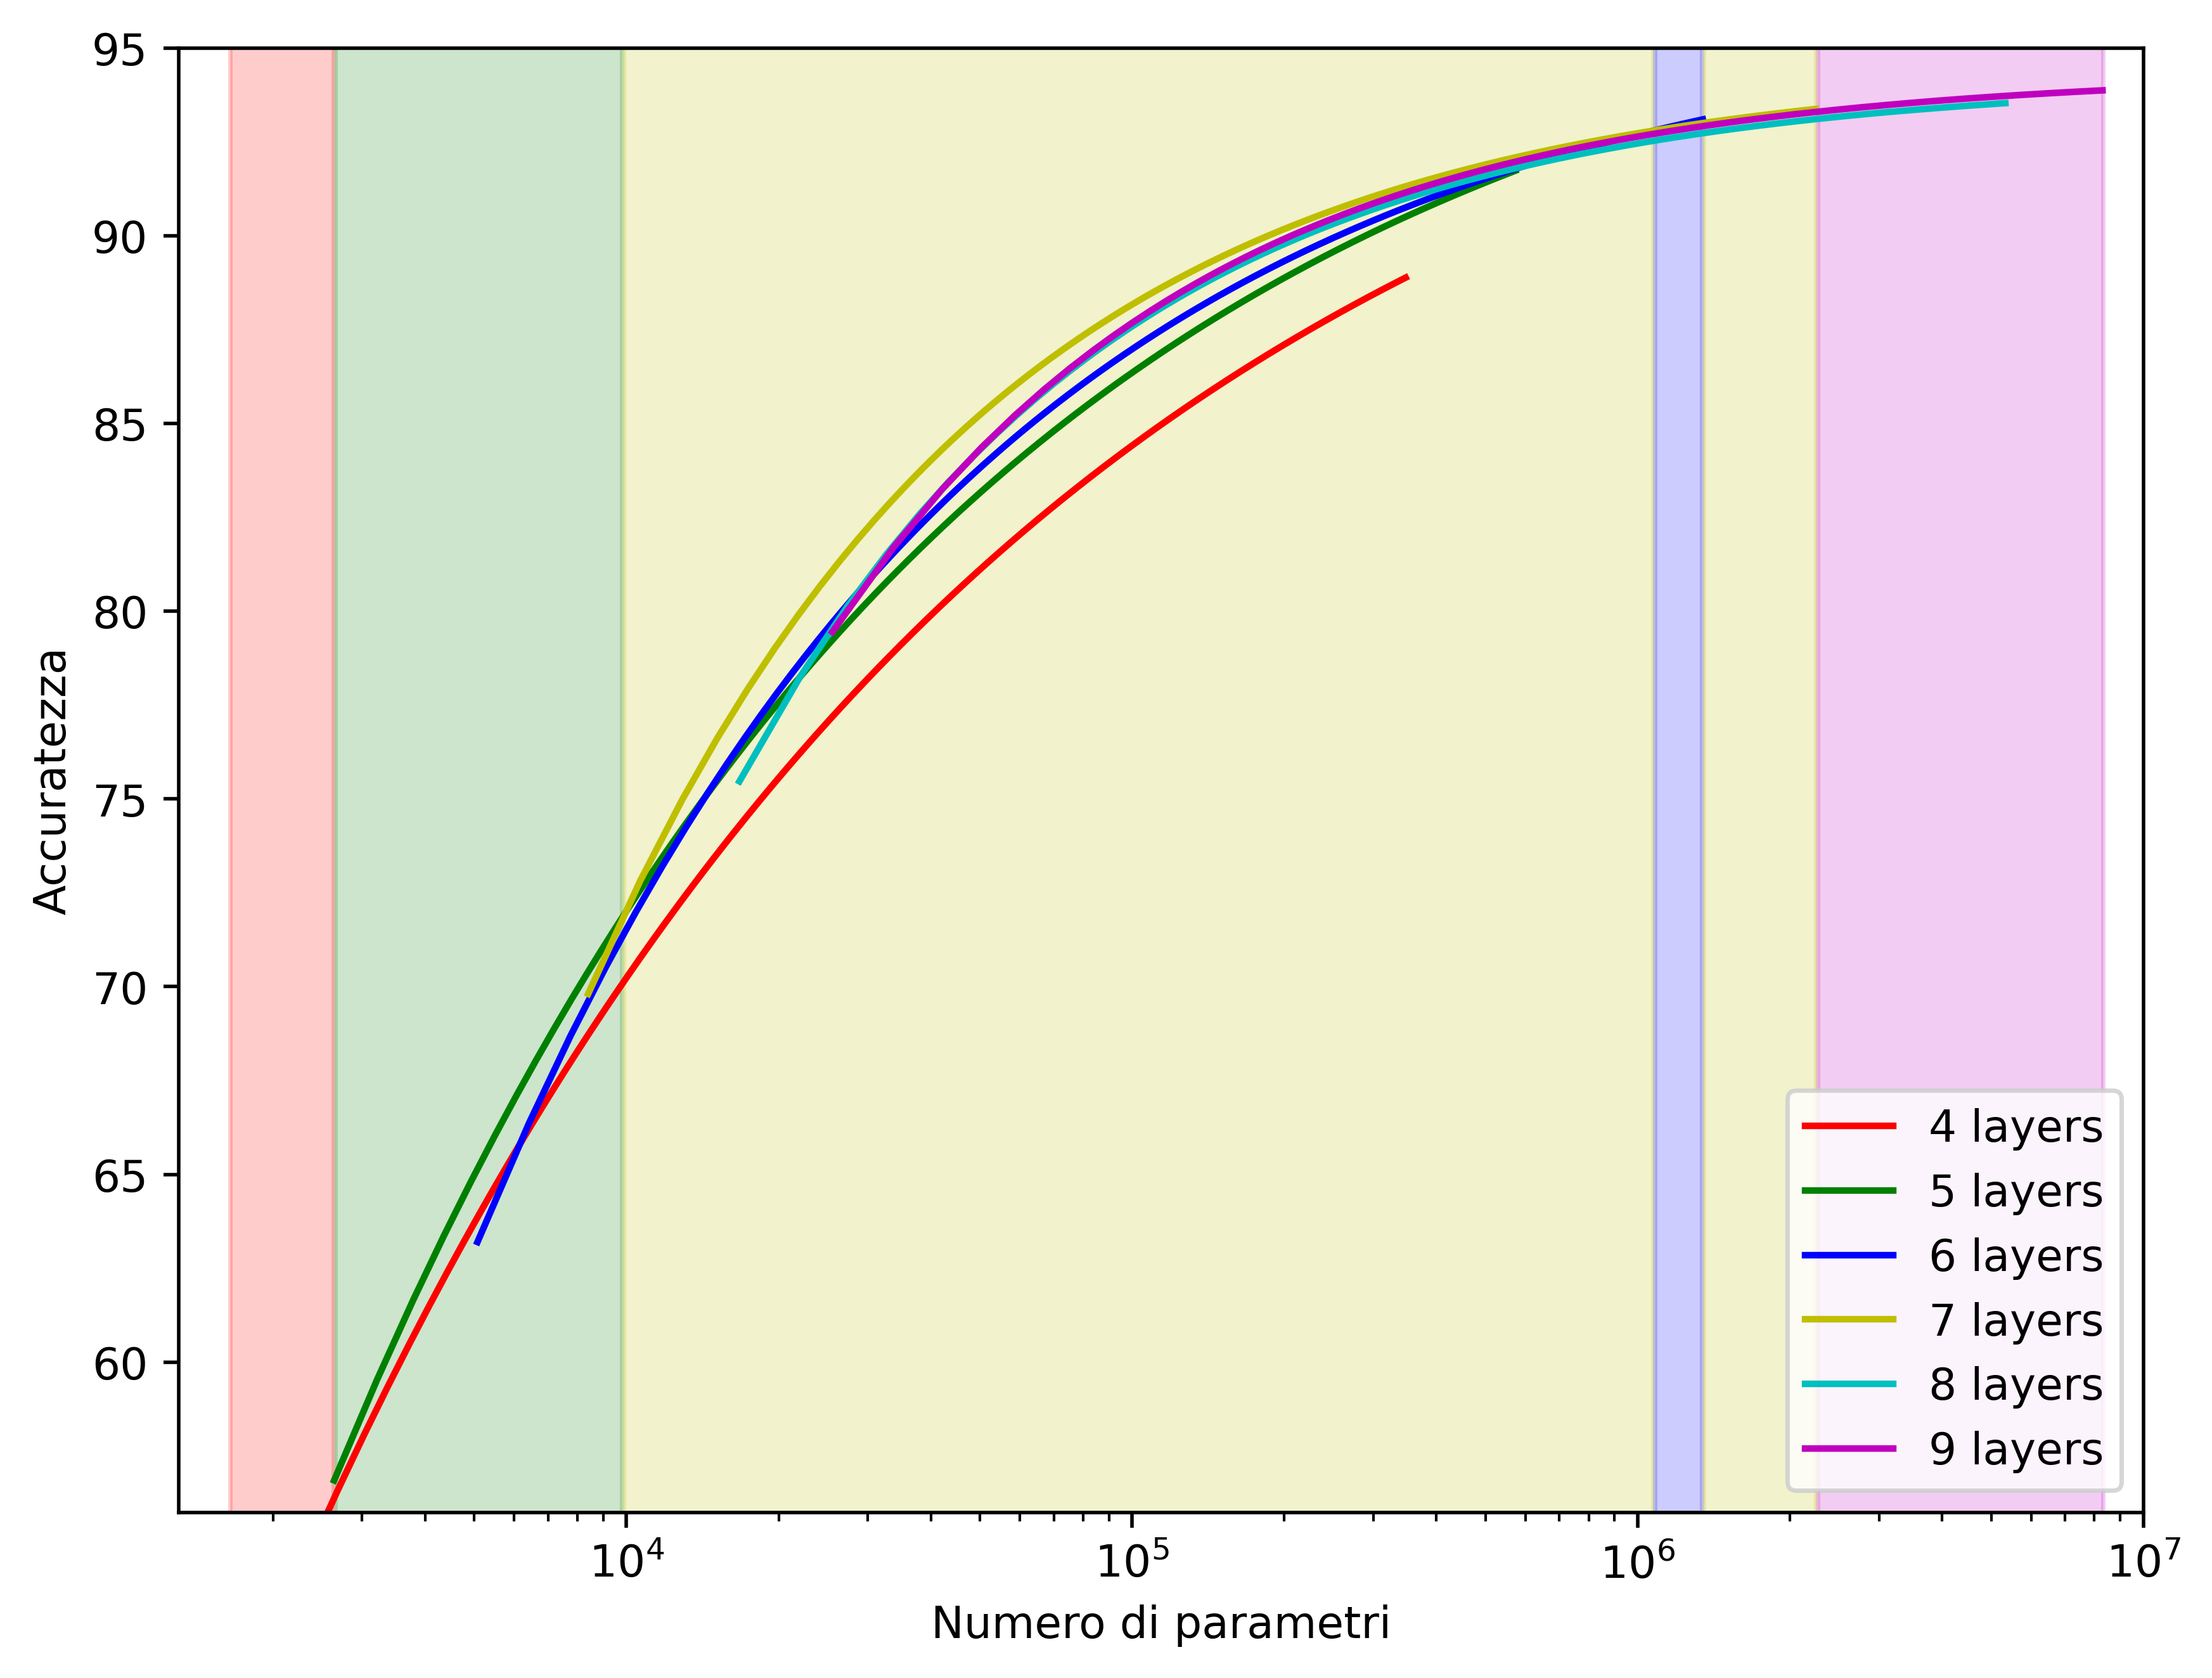
\includegraphics[width=0.31\textwidth]{tesi/immagini/segment_reg.png}}\quad
    \caption{\textit{Segmentazione e smoothing}. L'immagine (a) rappresenta graficamente la segmentazione eseguita sulla distribuzione di dati, (b) aggiunge il processo di smoothing, nella figura (c) la segmentazione è stata eseguita solamente basandosi sulle informazioni derivanti dalla funzione di regressione.}
    \label{fig:segmentation}
\end{figure}

% In questa situazione come ``ampiezza" si intende il logartimo in base 10 che ha come argomento il rapporto tra l'estremo superiore e quello inferiore del segmento; in particolare la threshold utilizzata assume il valore di $threshold=0.13$ ed un intervallo verrà quindi considerato da scartare quando $log_{10}\left( \frac{estremo\ superiore}{estremo\ inferiore} \right) < 0.13$.

\section{Valutazione dell'efficacia del Linear Probing}

Dato che è stato mostrato come la tecnica del Linear Probing (sezione \ref{sec:probes}) sia in grado di mostrare il contributo ed il ruolo di ogni layer all'interno di una rete convoluzionale, è ragionevole pensare che tale metodo possa anche aiutare ad analizzare e valutare le performance di determinati modelli di PhiNets per poter trarre una conclusioni su quale sia il miglior numero di strati convolutivi da scegliere.

Per poter mostrare come una determinata configurazione di iperparametri per una PhiNet con un certo budget di risorse computazionali sia più conveniente rispetto ad un'altra, sarebbe utile mostrare una qualche correlazione tra gli andamenti delle loss delle linear probes per specifici valori di numero di layer e le performance di classificazione finali della rete. 

In figura \ref{fig:probe_phinets} è mostrato l'andamento dei valori di loss per le linear probes applicate ad una PhiNet.

\begin{figure}[h!]
    \centering
    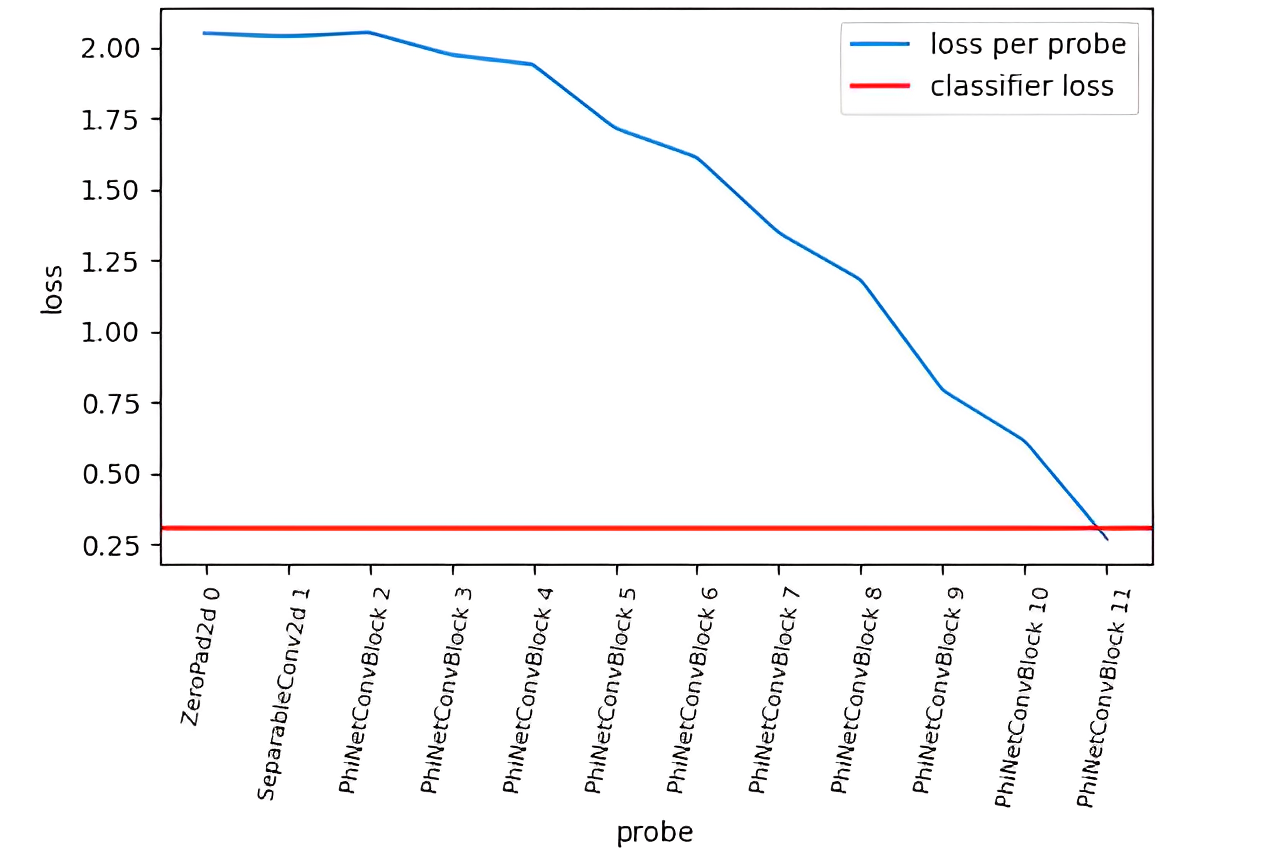
\psfig{file=immagini/loss_per_probe.png,width=0.4\textwidth}
    \caption{\textit{Loss per probe di una PhiNet}.}
    \label{fig:probe_phinets}
\end{figure}

A differenza di quanto visto nel grafico \ref{fig:probe}, che mostra i risultati dell'applicazione delle linear probes su una \textit{ResNet-50} \cite{ResNet}, nel caso delle PhiNets l'andamento mostrato dalla metrica di loss è monotono decrescente all'aumentare del blocco convoluzionale considerato. Dato che il trend monotono decrescente è comune alla quasi totalità dei modelli considerati, si può facilmente trarre la conclusione che l'architettura di rete delle PhiNets è particolarmente efficiente per il task di classificazione di immagini e che non sono presenti layer convolutivi che degradano le prestazioni. 

Tuttavia tale considerazione riguarda le performance generali delle reti e non tiene conto delle differenze di configurazione degli iperparametri, come ad esempio i diversi numeri di layer. Indagando più nello specifico non sono state però trovate metriche che mostrassero una chiara correlazione tra l'andamento della funzione di loss delle linear probes per determinati valori di numeri di layer e le prestazioni di classificazione delle reti.

Con ciò non si intende dire che le linear probes non siano uno strumento di analisi utile, ma solamente che non mostrano un chiaro supporto per il confronto tra modelli di PhiNets, e rimangono altresì una preziosa risorsa per il crescente trend dell'interpretabilità dei modelli nell'ambito delle reti convoluzionali.

%Grazie al fatto che è stato dimostrato che la funzione iperbolica generalizzata è quella che approssima meglio (tra quelle provate) l'andamento della distribuzione di dati, è ora possibile avere una previsione dell'accuratezza di classificazione di una PhiNet, da addestrare con la scelta di determinati parametri che ne definiscono il \textit{setup} (capitolo \ref{cha:setup}), senza il bisogno di attendere i lunghi e costosi tempi di training.